\documentclass[11pt,letterpaper,twoside,openright]{report}
\usepackage[utf8]{inputenc}
\usepackage[english]{babel}

%preámbulo configuración de página
\usepackage[width=165mm,top=15mm,bottom=25mm,bindingoffset=20mm,includehead]{geometry}

%Preámbulo de Color de texto =================================================================
\usepackage{color}
\definecolor{gray97}{gray}{.97}
\definecolor{gray75}{gray}{.75}
\definecolor{gray45}{gray}{.45}
\definecolor{verde}{rgb}{0.0, 0.5, 0.0}

%preámbulo captions==========================================================================
\usepackage{caption}
\captionsetup{margin=40pt,format=hang,indention=-.5cm,font={footnotesize, rm},labelfont=bf,labelsep=colon}

%preámbulo encabezados=======================================================================
\usepackage{fancyhdr}
\pagestyle{fancy}
\fancyhead{}
\fancyfoot{}
\fancyhead[RO,LE]{\thepage}
\fancyhead[LO]{\nouppercase{\rightmark}}
\fancyhead[RE]{\nouppercase{\leftmark}}
\setlength{\headheight}{15pt} 

%preambulo portada



%preámbulo matemáticas=======================================================================
%\spanishdecimal{.}
\usepackage{amsmath}
\usepackage{amsfonts}
\usepackage{amssymb}
\usepackage{amsthm}
\usepackage{dsfont}
\usepackage{mathrsfs}
\newcommand{\sign}[1]{\mathrm{sign(#1)}} 
\newcommand{\refe}[1]{(\ref{#1})}
\newcommand{\rojo}[1]{{\color{red} #1}}
\newcommand{\RE}{\mathbb{R}}
\newcommand{\sig}[2]{\lceil#1\rfloor^{#2}}
\newcommand{\abs}[2]{|#1|^{#2}}
\providecommand{\norm}[1]{\lVert#1\rVert}
\usepackage{color}   
\setcounter{MaxMatrixCols}{20}
%\decimalpoint


%preámbulo sistema internacional de unidades================================================
\usepackage{siunitx}


%preámbulo referencias========================================================================
\usepackage[numbers]{natbib}
%\bibliographystyle{plainnat}
%preámbulo Marcadores=======================================================================
\usepackage[hidelinks, breaklinks=true, backref=page,colorlinks=true,linkcolor=blue,citecolor=magenta]{hyperref}


%preámbulo de gráficos=========================================================================
\usepackage{graphicx}
\graphicspath{{figuras/}}
\usepackage{subfigure}
\usepackage{float}

%Preámbulo tabla=============================================================================
\usepackage{multirow, array}
\usepackage{booktabs}
\usepackage{colortbl}
\definecolor{SeaGreen}{rgb}{0.13, 0.7, 0.67}
\definecolor{Peach}{rgb}{0.97, 0.51, 0.47}
\definecolor{LimeGreen}{rgb}{0.31, 0.78, 0.47}
\definecolor{bananayellow}{rgb}{1.0, 0.88, 0.21}
\usepackage{enumerate}
%preámbulo de apéndices======================================================================
\usepackage[toc,page]{appendix}
\renewcommand{\appendixpagename}{Apéndices}

%preámbulo de url============================================================================
\usepackage{url}

%preámbulo de nomenclatura==================================================================
\usepackage[intoc,spanish]{nomencl}
\makenomenclature
\usepackage{etoolbox}


%Preámbulo para código de programación=======================================================
\usepackage{listings}
\lstset{ 
	backgroundcolor=\color{white},
	rulesepcolor=\color{black},
	%
	stringstyle=\ttfamily,
	showstringspaces = false,
	basicstyle=\footnotesize\ttfamily,
	commentstyle=\color{gray45},
	keywordstyle=\bfseries,
	%
}
\renewcommand{\lstlistingname}{Listado}

%Preámbulo numeros decimales================================================================
%\spanishdecimal{.}

%Redifiniendo Titulos==========================================================================
\usepackage{titlesec}
\newcommand{\bigrule}{\titlerule[0.5mm]}
\titleformat{\chapter}[display] % Se cambia el formato del capitulo
%{\bfseries\Huge} % por defecto se usarán caracteres de tamaño \Huge en negrita
{\bfseries\Huge} % por defecto se usarán caracteres de tamaño \Huge en negrita
{% contenido de la etiqueta
	\titlerule % línea horizontal
	\filright % texto alineado a la derecha
	\Large\chaptertitlename\ % "Capítulo" o "Apéndice" en tamaño \Large en lugar de \Huge
	\Large\thechapter} % número de capítulo en tamaño \Large
{0mm} % espacio mínimo entre etiqueta y cuerpo
{\filright} % texto del cuerpo alineado a la derecha
[\vspace{0.5mm} \bigrule] % después del cuerpo, dejar espacio vertical y trazar línea horizontal gruesa

%Preámbulo utilidades=========================================================================
\usepackage{pdfpages}	%Incluye hojas de de archivos PDF
\usepackage{siunitx}			%Sitema internacional de unidades
\usepackage[T1]{fontenc}	%Fuentes
\usepackage{textcomp}		%Fuentes

%preámbulo teoremas, Definiciones y Proposiciones ==============================================================================================================
\newtheorem{theorem}{Theorem}[chapter]
\newtheorem{definition}{Definition}[chapter]
\newtheorem{proposition}{Proposition}[chapter]
\newtheorem{observation}{Observation}[chapter]
\newtheorem{lemma}{Lemma}[chapter]
\newtheorem{property}{Property}[chapter]
\newtheorem{assumtion}{Assumption}[chapter]
\newtheorem{corollary}{Corollary}[chapter]

%preámbulo acronimo ===================================================
\usepackage{acronym}
\acrodef{fl}[FL]{Función de Lyapunov} \acused{fl}
\acrodef{pd}[p.d.]{positiva definida}
\acrodef{ae}[AE]{asintóticamente estable}
\acrodef{gae}[GAE]{global y asintóticamente estable}


%preámbulo de nomenclatura ==========================================
%\usepackage[intoc, spanish]{nomencl}
\makenomenclature
\nomenclature{$MCC$}{Modo de conducción continua}
%FIN DEL PREÁMBULO===================================================




%====================================================================
%====================================================================
%                                                  INICIO DEL DOCUMENTO
%====================================================================
%====================================================================
\begin{document}

%====================================================================
%                                                                      Macros
%====================================================================
%\newcommand{Nombre}{Formula- Imagen lo que seas}

%====================================================================
%                        Portada
%====================================================================
\thispagestyle{empty}

\begin{titlepage}
	%\newgeometry{top=2.4cm,hmargin=3.7cm,bottom=2.4cm}
	%\thispagestyle{empty}
	
	\begin{center}
		
\includegraphics[height=4.5cm]{UNAM.png}	
	\end{center}
	%	\begin{figure}[ht]
		%		\minipage{0.76\textwidth}
		%		
\includegraphics[width=4cm]{UNAM.png}
		%		\label{EscudoUNAM}
		%		\endminipage
		%		\minipage{0.32\textwidth}
		%		
\includegraphics[height = 4cm ,width=3.5cm]{FI.jpg}
		%		\label{EscudoFC}
		%		\endminipage
		%	\end{figure}
	
	\begin{center}
		%		
\includegraphics[height=3.5cm]{unam_azul.pdf}\\
		%		\vspace{1cm}
		\textbf{{\Large UNIVERSIDAD NACIONAL AUTÓNOMA DE MÉXICO}}\\
		PROGRAMA DE MAESTRÍA Y DOCTORADO EN INGENIERÍA\\
		INGENIERÍA ELÉCTRICA – CONTROL\\
		\vspace{2cm}
		\textbf{APLICACIÓN DE MEDICIONES DE VECTORES INERCIALES EN EL CONTROL DE SEGUIMIENTO DE UN UAV QUADROTOR: UN ENFOQUE EXPERIMENTAL}
		\\
		\vspace{2cm}
		TESIS\\
		QUE PARA OPTAR POR EL GRADO DE:\\
		MAESTRO EN INGENIERÍA\\
		\vspace{2cm}
		PRESENTA:\\
		JORGE MANUEL VILLARREAL MALDONADO\\
		\vspace{1.8cm}
		TUTOR PRINCIPAL\\
		DR. YU TANG XU\\
		FACULTAD DE INGENIERÍA, UNAM\\
		
		\vspace{1.8cm}
		CIUDAD UNIVERSITARIA, CD. MX. SEPTIEMBRE 2, 2023\\
	\end{center}
	
\end{titlepage}

		%\begin{center}
		%	
\includegraphics[height=4.5cm]{UNAM.png}	
		%\end{center}
		%%	\begin{figure}[ht]
		%	%		\minipage{0.76\textwidth}
		%	%		
\includegraphics[width=4cm]{UNAM.png}
		%	%		\label{EscudoUNAM}
		%	%		\endminipage
		%	%		\minipage{0.32\textwidth}
		%	%		
\includegraphics[height = 4cm ,width=3.5cm]{FI.jpg}
		%	%		\label{EscudoFC}
		%	%		\endminipage
		%	%	\end{figure}
		%
		%\begin{center}
		%	
		%	\textbf{{\large UNIVERSIDAD NACIONAL AUTÓNOMA DE MÉXICO}}\\
		%	MASTER AND DOCTORATE PROGRAM IN ENGINEERING\\
		%	ELECTRICAL ENGINEERING - CONTROL\\
		%	\vspace{2cm}
		%	{\large BL-HOMOGENEOUS SLIDING-MODE OBSERVERS DESIGN \\
		%		FOR MIMO LINEAR SYSTEMS}
		%	\\
		%	\vspace{2cm}
		%	\textbf{THESIS}\\
		%	PRESENTED FOR THE DEGREE OF\\
		%	MASTER IN ENGINEERING\\
		%	\vspace{2cm}
		%	PRESENTS:\\
		%	\textbf{RENE MELENDEZ PEREZ}\\
		%	\vspace{1.8cm}
		%	PRINCIPAL DIRECTOR\\
		%	\textbf{DR. LEONID FRIDMAN}\\FACULTY OF ENGINEERING, UNAM\\
		%	
		%	\vspace{1.8cm}
		%	MEXICO CITY, JULY 2022\\
		%\end{center}

\newpage
\thispagestyle{empty}
$\ $


\newpage
\thispagestyle{empty}
\vspace{30mm}

\noindent JURADO ASIGNADO:
\vspace{8mm}

\begin{tabbing}
%	Presidente: \ \ \ \ \ \ \ \=Dr. Arteaga Pérez Marco Antonio \\ [3mm]
%	Secretario: \> Dr. Moreno Pérez Jaime Alberto\\ [3mm]
%	1er. Vocal: \> Dr. Fridman Leonid\\ [3mm]
%	2o. Vocal: \> Dr. Rocha Cózatl Edmundo Gabriel\\ [3mm]
%	3er. Vocal: \> Dr. Dávila Montoya Jorge Ángel\\ [12mm]
\end{tabbing}

\vspace{1.5cm}
\noindent La tesis se realizó en el Posgrado de Ingeniería, UNAM.\\

\begin{center}
	TUTOR  DE  TESIS:\\\vspace{.04cm}
	DR. YU TANG XU\\
	\vspace{2cm}
	--------------------------------------------------\\
	FIRMA
\end{center}

\newpage
\thispagestyle{empty}
%$\ $
%====================================================================
%    


\newpage
%\chapter*{Acknowledgment} 
\begin{flushright}
\textit{To my family for their unconditional support.}\vspace{0.5cm}

\textit{To Dr. Leonid Fridman and Dr. Jaime Moreno for their support, and their fundamental contribution \\ in the development and guidance in this thesis. \\ But above all, for the knowledge transmitted over these two years.}\vspace{0.5cm}

\textit{To my colleagues in the sliding mode group for their advice and feedback.}\vspace{0.5cm}

\textit{To the graduate program in electrical engineering and its professors.}\vspace{0.5cm}

\textit{And, to UNAM for opening the doors and the support provided.}

\end{flushright}

 
\chapter*{Agradecimientos} 
\thispagestyle{empty}
\begin{flushright}

\end{flushright}
\newpage
\thispagestyle{empty}
$\ $   
    
    
\newpage
%\chapter*{Acknowledgment} 
\begin{flushright}
\textit{To my family for their unconditional support.}\vspace{0.5cm}

\textit{To Dr. Leonid Fridman and Dr. Jaime Moreno for their support, and their fundamental contribution \\ in the development and guidance in this thesis. \\ But above all, for the knowledge transmitted over these two years.}\vspace{0.5cm}

\textit{To my colleagues in the sliding mode group for their advice and feedback.}\vspace{0.5cm}

\textit{To the graduate program in electrical engineering and its professors.}\vspace{0.5cm}

\textit{And, to UNAM for opening the doors and the support provided.}

\end{flushright}

 
\chapter*{Acknowledgment} 
\thispagestyle{empty}
\begin{flushright}
	
\end{flushright}
\newpage
\thispagestyle{empty}
$\ $

\chapter*{Resumen} % si no queremos que a�ada la palabra "Capitulo"
\markboth{Resumen}{Resumen} % encabezado

Una bonita historia

\newpage
%\chapter*{Acknowledgment} 
\begin{flushright}
\textit{To my family for their unconditional support.}\vspace{0.5cm}

\textit{To Dr. Leonid Fridman and Dr. Jaime Moreno for their support, and their fundamental contribution \\ in the development and guidance in this thesis. \\ But above all, for the knowledge transmitted over these two years.}\vspace{0.5cm}

\textit{To my colleagues in the sliding mode group for their advice and feedback.}\vspace{0.5cm}

\textit{To the graduate program in electrical engineering and its professors.}\vspace{0.5cm}

\textit{And, to UNAM for opening the doors and the support provided.}

\end{flushright}

 
\chapter*{Abstract} 
This study focuses on the experimental implementation and detailed analysis of a tracking controller for a quadrotor unmanned aerial vehicle (UAV), specifically the Bebop 2 model. The initial controller design consists of two essential components: an outer saturated position control loop and an inner attitude control loop. The former is tasked with defining a thrust direction free from singularities, thereby ensuring global exponential tracking. On the other hand, the inner attitude control is grounded on precise inertial vector measurements and gyro rates, enabling accurate tracking of the desired attitude for the UAV's proper positioning.

To ensure the efficacy and robustness of the proposed controller, a three-phase testing protocol was established. The first phase involved computational simulations conducted in MATLAB, primarily aimed at corroborating and refining the controller's theoretical data. Once these results were validated, the study progressed to the second phase, which entailed the creation of a controlled simulation environment in ROS and Gazebo. This more advanced simulation incorporated real parameters and was based on the technical and behavioral specifications of the Bebop 2 drone, allowing for a closer approximation to real flight conditions.

The third and final phase marked the culmination of the project: the implementation and testing of the controller in a real environment using the Bebop 2 drone. Trials in this setting not only validated the controller's efficacy under real conditions but also assessed its robustness against potential disturbances and variables not considered in the simulations.

The results obtained throughout these phases demonstrate that the proposed controller is not only effective in theory but also applicable and reliable in practical scenarios, offering a robust solution for tracking and controlling quadrotor UAVs under various conditions.

\newpage
\thispagestyle{empty}
$\ $


%====================================================================

%\tableofcontents % indice de contenidos


\tableofcontents % indice de contenidos
\thispagestyle{empty}

%Índice de Figuras====================================================================================================
%\listoffigures % indice de figuras
\addcontentsline{toc}{chapter}{\'List of Figures} % para que aparezca en el indice de contenidos

\listoffigures % indice de figuras
\addcontentsline{toc}{chapter}{List of Figures} % para que aparezca en el indice de contenidos
\setcounter{page}{1}
\pagenumbering{Roman} 

%Lista de Acrónimos =====================================================================================================
%\chapter*{List of acronyms} % Lista de acrónimos
\addcontentsline{toc}{chapter}{Lista de acrónimos} % para que aparezca en el indice de contenidos
\markboth{Lista de acrónimos}{Lista de acrónimos}
\begin{tabular}{cl}
	HOSM	&\hspace{1.5cm} Higher-Order Sliding Modes\\
			&\hspace{1.5cm} (\textit{Modos Deslizantes de Orden Superior})\\\\
	UIO		&\hspace{1.5cm} Unknown Input Observer	\\
			&\hspace{1.5cm} (\textit{Observador con Entradas Desconocidas})\\\\
	SMO		&\hspace{1.5cm} Sliding Mode Observer\\
			&\hspace{1.5cm} (\textit{Observador por Modos Deslizantes})\\\\
	Bl		&\hspace{1.5cm} Homogeneous in the bi-limit\\
			&\hspace{1.5cm} (\textit{Observador por Modos Deslizantes})\\\\
	LTI	   	&\hspace{1.5cm} Linear Time Invariant \\
			&\hspace{1.5cm} (\textit{Lineal Invariante en el Tiempo})\\\\
	SCB	   	&\hspace{1.5cm} Special Coordinate Basis\\
			&\hspace{1.5cm} (\textit{Base en Coordenadas Especiales})\\\\
	MIMO	&\hspace{1.5cm} Multiple-input Multiple-output\\
			&\hspace{1.5cm} (\textit{Múltiple entrada múltiple salida})\\\\
	LF		&\hspace{1.5cm} Lyapunov Function\\
			&\hspace{1.5cm} (\textit{Función de Lyapunov})\\\\
	Bl-LF	&\hspace{1.5cm} Bl-homogeneous Lyapunov Function\\
			&\hspace{1.5cm} (\textit{Función de Lyapunov})\\\\
	SM		&\hspace{1.5cm} Sliding mode\\
			&\hspace{1.5cm} (\textit{Modos deslizantes})	
\end{tabular}

\chapter*{List of acronyms} % Lista de acrónimos
\addcontentsline{toc}{chapter}{List of acronyms} % para que aparezca en el indice de contenidos
\markboth{List of acronyms}{List of acronyms}
\begin{tabular}{cl}
	HOSM	&\hspace{1.5cm} Higher-Order Sliding Modes\\\\
	UIO		&\hspace{1.5cm} Unknown Input Observer	\\\\
	SMO		&\hspace{1.5cm} Sliding Mode Observer \\\\
	Bl		&\hspace{1.5cm} Bi-limit\\\\
	LTI	   	&\hspace{1.5cm} Linear Time Invariant \\\\
	SCB	   	&\hspace{1.5cm} Special Coordinate Basis\\\\
	MIMO	&\hspace{1.5cm} Multiple-input Multiple-output\\\\
	LF		&\hspace{1.5cm} Lyapunov Function\\\\
	Bl-LF	&\hspace{1.5cm} Bl-homogeneous Lyapunov Function\\\\
	SM		&\hspace{1.5cm} Sliding mode\\\\
	FT		&\hspace{1.5cm} Finite-Time\\\\
	FxT		&\hspace{1.5cm} Fixed-Time\\\\
	RED		&\hspace{1.5cm} Robust Exact Differentiator\\\\
	OMC		&\hspace{1.5cm} Observer Matching Condition \\\\
	ISS		&\hspace{1.5cm} Input to State Stability \\\\
\end{tabular}


%Nomenglatura =====================================================================================================

%\printnomenclature


% Capitulos ==========================================================================================================

\chapter{Introducción}
\setcounter{page}{1}
\renewcommand{\thepage}{\arabic{page}}


%%%%%%%%%%%%%%%%%%%%%%%%%%%%%%%%%%%%%%%%%%%%%%%%%%%%%%%5
% Motivacion
%%%%%%%%%%%%%%%%%%%%%%%%%%%%%%%%%%%%%%%%%%%%%%%%%%%%%%%%%5
\section{Motivación}
En el vasto panorama de la investigación científica y tecnológica contemporánea, el control de vehículos aéreos no tripulados (UAVs) se ha consolidado como una de las áreas más prometedoras y dinámicas. Esta destacada posición no es mera coincidencia; es el resultado de una serie de avances tecnológicos, industriales y académicos que han convergido en las últimas dos décadas. La aspiración de lograr una autonomía total en estos vehículos no es meramente una ambición académica, sino que tiene profundas implicaciones para una amplia gama de aplicaciones en diversos campos, desde la agricultura y la logística hasta la vigilancia y el entretenimiento.

Dentro del espectro de UAVs, los vehículos de despegue y aterrizaje vertical (VTOL), especialmente los quadrotors, han emergido como objetos de estudio particularmente intrigantes. Su versatilidad inherente, combinada con los desafíos teóricos y prácticos que presentan, los convierte en candidatos ideales para la investigación avanzada. Sin embargo, es precisamente esta complejidad la que ha revelado una serie de brechas en la literatura existente.

A pesar de los avances teóricos significativos, una observación crítica revela que gran parte de la investigación previa opera bajo supuestos ideales, comúnmente distantes de las particularidades y obstáculos de los ambientes reales. Las perturbaciones ambientales, las mediciones ruidosas, la incertidumbre paramétrica y otros factores impredecibles pueden desafiar y, en ocasiones, invalidar los modelos teóricos.

En este contexto, el presente trabajo se propone como una contribución esencial al campo. No se limita a abordar los desafíos teóricos del control de UAVs, sino que se aventura con determinación en el mundo experimental, buscando validar, refinar y, si es necesario, redefinir los paradigmas existentes. Esta transición de la teoría a la experimentación no es un mero ejercicio académico, sino un requisito esencial para asegurar que los modelos y controladores propuestos sean sólidos, duraderos y, primordialmente, funcionales en contextos reales.

La motivación que impulsa este trabajo es, por lo tanto, multifacética. Por un lado, yace la aspiración de aportar de manera sustancial al cuerpo teórico del control de UAVs, introduciendo propuestas vanguardistas y enfrentando vacíos presentes. Por otro lado, hay un reconocimiento explícito de la importancia crítica de la validación experimental. En última instancia, este trabajo aspira a ser un puente entre la teoría y la práctica, reafirmando que la verdadera medida de cualquier avance teórico reside en su capacidad para enfrentar y superar los desafíos del mundo real.


%%%%%%%%%%%%%%%%%%%%%%%%%%%%%%%%%%%%%%%%%%%%%%%%%%%%%%%5
%   Antecedentes
%%%%%%%%%%%%%%%%%%%%%%%%%%%%%%%%%%%%%%%%%%%%%%%%%%%%%%%%%5
\section{Antecedentes}

El control de vehículos aéreos no tripulados (UAVs) ha sido objeto de intensa investigación en las últimas décadas. Estos sistemas, que alguna vez fueron relegados a aplicaciones militares o de nicho, han encontrado un lugar en una variedad de industrias, desde la agricultura hasta la entrega de paquetes y la cinematografía.

Los UAVs, en particular los de despegue y aterrizaje vertical (VTOL) como los quadrotors, han capturado la atención de los investigadores y entusiastas por igual debido a su versatilidad y capacidad para operar en entornos que otros vehículos aéreos podrían encontrar desafiantes. Sin embargo, con esta versatilidad viene una serie de desafíos únicos en términos de control y estabilidad, especialmente dada la naturaleza subactuada de estos vehículos.

A lo largo de los años, se han propuesto numerosas técnicas para abordar estos desafíos. El enfoque de empuje vectorizado ha sido una solución popular. Sin embargo, un aspecto esencial y emergente en la literatura reciente es la propuesta de utilizar mediciones vectoriales para determinar la actitud del UAV. Esta metodología, que se aleja de las técnicas tradicionales basadas en matrices de rotación, cuaterniones unitarios o ángulos de Euler, ha demostrado ser prometedora.

A pesar de estos avances, ha habido una tendencia en la literatura a operar bajo supuestos ideales, a menudo sin considerar las complejidades y desafíos de los entornos operativos reales. Las perturbaciones ambientales, las mediciones ruidosas y la incertidumbre paramétrica son solo algunos de los factores que pueden afectar la eficacia de los controladores teóricos en situaciones prácticas.

En este contexto, surge la necesidad de investigaciones que no solo aborden los desafíos teóricos asociados con el control de UAVs, sino que también consideren la transición de estos modelos teóricos al ámbito experimental. La validación en entornos reales es esencial para garantizar que los controladores propuestos sean robustos y aplicables en situaciones prácticas.
%%%%%%%%%%%%%%%%%%%%%%%%%%%%%%%%%%%%%%%%%%%%%%%%%%%%%%%5
%   Formulacion del problema
%%%%%%%%%%%%%%%%%%%%%%%%%%%%%%%%%%%%%%%%%%%%%%%%%%%%%%%%%5
\section{Formulación del problema}

%%%%%%%%%%%%%%%%%%%%%%%%%%%%%%%%%%%%%%%%%%%%%%%%%%%%%%%%%%%%%5
% Objetivos
%%%%%%%%%%%%%%%%%%%%%%%%%%%%%%%%%%%%%%%%%%%%%%%%%%%%%%%%5
\section{Objetivos}
El presente trabajo de tesis tiene como objetivos:
\begin{itemize}
  \item D
  \item P
  \item I
  \item E
\end{itemize}

%%%%%%%%%%%%%%%%%%%%%%%%%%%%%%%%%%%%%%%%%%%%%%%%%%%%%%%5
%   Contribuciones
%%%%%%%%%%%%%%%%%%%%%%%%%%%%%%%%%%%%%%%%%%%%%%%%%%%%%%%%%5
\section{Contribuciones}
\begin{itemize}
    \item Encontrar condiciones para obtener 
    \item P
    \item I
    \item E
  \end{itemize}

%%%%%%%%%%%%%%%%%%%%%%%%%%%%%%%%%%%%%%%%%%%%%%%%%%%%%%%5
% Organizacion de la tesis
%%%%%%%%%%%%%%%%%%%%%%%%%%%%%%%%%%%%%%%%%%%%%%%%%%%%%%%%%5
\section{Organización de la tesis}
El presente trabajo de tesis se encuentra dividido en cinco capítulos,
siendo el presente el que concierne a la introducción. Los siguientes cuatro
 se describen a continuación:\\

En el \textbf{Capítulo 2}, se presenta el marco teórico 

En el \textbf{Capítulo 3}, se presenta 
Para validar el funcionamiento del gemelo digital, en el \textbf{Capítulo 4} 


\documentclass[11pt,letterpaper,twoside,openright]{report}
\usepackage[utf8]{inputenc}
\usepackage[english]{babel}

%preámbulo configuración de página
\usepackage[width=165mm,top=15mm,bottom=25mm,bindingoffset=20mm,includehead]{geometry}

%Preámbulo de Color de texto =================================================================
\usepackage{color}
\definecolor{gray97}{gray}{.97}
\definecolor{gray75}{gray}{.75}
\definecolor{gray45}{gray}{.45}
\definecolor{verde}{rgb}{0.0, 0.5, 0.0}

%preámbulo captions==========================================================================
\usepackage{caption}
\captionsetup{margin=40pt,format=hang,indention=-.5cm,font={footnotesize, rm},labelfont=bf,labelsep=colon}

%preámbulo encabezados=======================================================================
\usepackage{fancyhdr}
\pagestyle{fancy}
\fancyhead{}
\fancyfoot{}
\fancyhead[RO,LE]{\thepage}
\fancyhead[LO]{\nouppercase{\rightmark}}
\fancyhead[RE]{\nouppercase{\leftmark}}
\setlength{\headheight}{15pt} 


%preámbulo matemáticas=======================================================================
%\spanishdecimal{.}
\usepackage{amsmath}
\usepackage{amsfonts}
\usepackage{amssymb}
\usepackage{dsfont}
\usepackage{mathrsfs}
\newcommand{\sign}[1]{\mathrm{sign(#1)}} 
\newcommand{\refe}[1]{(\ref{#1})}
\newcommand{\rojo}[1]{{\color{red} #1}}
\newcommand{\RE}{\mathbb{R}}
\newcommand{\sig}[2]{\lceil#1\rfloor^{#2}}
\newcommand{\abs}[2]{|#1|^{#2}}
\providecommand{\norm}[1]{\lVert#1\rVert}
\usepackage{color}   
\setcounter{MaxMatrixCols}{20}
%\decimalpoint


%preámbulo sistema internacional de unidades================================================
\usepackage{siunitx}


%preámbulo referencias========================================================================
\usepackage[numbers]{natbib}
%\bibliographystyle{plainnat}
\usepackage[hidelinks, breaklinks=true, backref=page,colorlinks=true,linkcolor=blue,citecolor=magenta]{hyperref}


%preámbulo de gráficos=========================================================================
\usepackage{graphicx}
\graphicspath{{figuras/}}
\usepackage{subfigure}
\usepackage{float}

%Preámbulo tabla=============================================================================
\usepackage{multirow, array}
\usepackage{booktabs}
\usepackage{colortbl}
\definecolor{SeaGreen}{rgb}{0.13, 0.7, 0.67}
\definecolor{Peach}{rgb}{0.97, 0.51, 0.47}
\definecolor{LimeGreen}{rgb}{0.31, 0.78, 0.47}
\definecolor{bananayellow}{rgb}{1.0, 0.88, 0.21}
%preámbulo de apéndices======================================================================
\usepackage[toc,page]{appendix}
\renewcommand{\appendixpagename}{Apéndices}

%preámbulo de url============================================================================
\usepackage{url}

%preámbulo de nomenclatura==================================================================
\usepackage[intoc,spanish]{nomencl}
\makenomenclature
\usepackage{etoolbox}


%Preámbulo para código de programación=======================================================
\usepackage{listings}
\lstset{ 
	backgroundcolor=\color{white},
	rulesepcolor=\color{black},
	%
	stringstyle=\ttfamily,
	showstringspaces = false,
	basicstyle=\footnotesize\ttfamily,
	commentstyle=\color{gray45},
	keywordstyle=\bfseries,
	%
}
\renewcommand{\lstlistingname}{Listado}

%Preámbulo numeros decimales================================================================
%\spanishdecimal{.}


%preámbulo Marcadores=======================================================================
\usepackage[hidelinks, breaklinks=true, backref=page]{hyperref} 

%Redifiniendo Titulos==========================================================================
\usepackage{titlesec}
\newcommand{\bigrule}{\titlerule[0.5mm]}
\titleformat{\chapter}[display] % Se cambia el formato del capitulo
%{\bfseries\Huge} % por defecto se usarán caracteres de tamaño \Huge en negrita
{\bfseries\Huge} % por defecto se usarán caracteres de tamaño \Huge en negrita
{% contenido de la etiqueta
	\titlerule % línea horizontal
	\filright % texto alineado a la derecha
	\Large\chaptertitlename\ % "Capítulo" o "Apéndice" en tamaño \Large en lugar de \Huge
	\Large\thechapter} % número de capítulo en tamaño \Large
{0mm} % espacio mínimo entre etiqueta y cuerpo
{\filright} % texto del cuerpo alineado a la derecha
[\vspace{0.5mm} \bigrule] % después del cuerpo, dejar espacio vertical y trazar línea horizontal gruesa

%Preámbulo utilidades=========================================================================
\usepackage{pdfpages}	%Incluye hojas de de archivos PDF
\usepackage{siunitx}			%Sitema internacional de unidades
\usepackage[T1]{fontenc}	%Fuentes
\usepackage{textcomp}		%Fuentes

%preámbulo teoremas, Definiciones y Proposiciones ==============================================================================================================
\newtheorem{theorem}{Theorem}[chapter]
\newtheorem{definition}{Definition}[chapter]
\newtheorem{proposition}{Proposition}[chapter]
\newtheorem{observation}{Observation}[chapter]
\newtheorem{lemma}{Lemma}[chapter]
\newtheorem{property}{Property}[chapter]
\newtheorem{assumtion}{Assumption}[chapter]
\newtheorem{corollary}{Corollary}[chapter]

%preámbulo acronimo ===================================================
\usepackage{acronym}
\acrodef{fl}[FL]{Función de Lyapunov} \acused{fl}
\acrodef{pd}[p.d.]{positiva definida}
\acrodef{ae}[AE]{asintóticamente estable}
\acrodef{gae}[GAE]{global y asintóticamente estable}


%preámbulo de nomenclatura ==========================================
%\usepackage[intoc, spanish]{nomencl}
\makenomenclature
\nomenclature{$MCC$}{Modo de conducción continua}
%FIN DEL PREÁMBULO===================================================

%====================================================================
%====================================================================
%                    INICIO DEL DOCUMENTO
%====================================================================
%====================================================================
\begin{document}
	\chapter{Preliminaries and Theoretical framework}	
In this chapter some definitions and a brief review of necessary mathematical tools will be given in order to have a clear exposition of the problem and results. First we start with the description of systems we are working on and the Special Coordinated Basis (SCB) transformation of linear systems, required in this work to the observer design. Then we recall the well known concepts of strong observability and strong detectability giving a characterization of them in terms of the zeros and relative degree of the system. Later we state the concepts of classical and weighted homogeneity and some relevant results in functional analysis with this property, immediately we give an extension to homogeneity in the bi-limit which is part of the central axis of this work. Additionally we have to remember a few important ideas on the Lyapunov stability issue, some recent concepts such as Finite Time Stability (FTS) and Fixed Time Stability are given formally. Finally we explain how the recently introduced Bl-homogeneous differentiators are built.

Although they have already been used in the previous chapter, some important notations are as follows. For a real variable $z\in \mathbb{R}$ and a real number $p\in \mathbb{R}$ the symbol $\sig{z}{p}=\abs{z}{p}\sign{z}$ is the signed power $p$ of $z$. According to this $\sig{z}{0}=\sign{z}$, additionally $\frac{d}{dz}\sig{z}{m}=m\abs{z}{m-1}$ and $\frac{d}{dz}\abs{z}{m}=m\sig{z}{m-1}$. Note that $\sig{z}{2}=\abs{z}{2}\sign{z} \neq z^2$, and if $p$ is an odd number then $\sig{z}{p}=z^p$ and $\abs{z}{p}=z^p$ for any even integer $p$. Moreover, $\sig{z}{p}\sig{z}{q}=\abs{z}{p+q}$, $\sig{z}{p}\sig{z}{0}=\abs{z}{p}$ and $\sig{z}{0}\abs{z}{p}=\sig{z}{p}$.

\section{Description of systems and properties}
In contrast to the Single Input - Single Output (SISO) case, in the Multi Input - Multi Output (MIMO) case existing normal forms are not clearly defined in order to design Unknown Input Observers (UIO) for example the well-known classical observability canonical form by Luenberger \cite{Luenberger1967}\cite{Gupta1974} which is based on the observability indices does not take the impact of the unknown inputs into account.

\subsection{Special Coordinated Basis} 
Essentially, the so-called Special Coordinate Basis \cite{Chen2004}\cite{Sannuti1986} decomposes the multivariable linear system into coupled chains of integrators. Such that several fundamental properties of linear systems regarding controllability (stabilisability), observability (detectability), invariant zeros, decoupling zeros, infinite zero structure, effect of feedback on zero structure, squaring down, diagonal and triangular decoupling, etc. can be directly displayed in terms of the Special Coordinate Basis.

Consider a general strictly proper linear system $\Sigma$ characterized by
\begin{equation}
	\begin{split}\label{ecu: Sigma}
		\Sigma: \left\{
		\begin{array}{rl}
			\dot{x} & =Ax+Du \\
			y & = Cx
		\end{array}
		\right. \\
	\end{split}
\end{equation}

where $x\in \RE^n, u\in \RE^m$ and $y\in \RE^p$ are the state, input and output respectively. Without loss of generality, we assume that all inputs and outputs are linearly independent, i.e. both $D$ and $C$ are of full rank. Then we have the following structural or Special Coordinate Basis decomposition of $\Sigma$.

\begin{theorem}\label{theorem: SCB}
	Consider the strictly proper system $\Sigma$ characterized by \eqref{ecu: Sigma SCB}. There exist a nonsingular state transformation, $\Gamma_s \in \RE^{n\times n}$ , a nonsingular output transformation, $\Gamma_o \in \RE^{p\times p}$, and a nonsingular input transformation, $\Gamma_i \in \RE^{m\times m}$, that will reveal all the structural properties $\Sigma$. More specifically, we have
	
	\begin{equation}
		x=\Gamma_s\bar{x}, \quad y=\Gamma_o\bar{y}, \quad u=\Gamma_i\bar{u},
	\end{equation}

which transform the system into 

\begin{equation}
	\begin{split}\label{ecu: Sigma SCB}
		\Sigma_{SCB}: \left\{
		\begin{array}{rl}
			\dot{\bar{x}} & =\bar{A}\bar{x}+\bar{D}\bar{u} \\
			\bar{y} & = \bar{C}\bar{x}
		\end{array}
		\right. \\
	\end{split}
\end{equation}

with the new state variables 
\begin{equation}
	\bar{x}=
	\begin{bmatrix}
		x_a \\
		x_b \\
		x_c \\
		x_d
	\end{bmatrix}, x_a \in \mathbb{R}^{n_a}, \quad x_b \in \mathbb{R}^{n_b}, \quad x_c \in \mathbb{R}^{n_c}, \quad x_d \in \mathbb{R}^{n_d}
\end{equation}

the new output variables 
\begin{equation}
	\bar{y}=
	\begin{bmatrix}
		y_d \\
		y_b
	\end{bmatrix}, y_d \in \mathbb{R}^{p_d}, \quad y_b \in \mathbb{R}^{p_b}
\end{equation}
and the new input variables
\begin{equation}
	\bar{u}=
	\begin{bmatrix}
		u_d \\
		u_c
	\end{bmatrix}, u_d \in \mathbb{R}^{p_d}, \quad u_c \in \mathbb{R}^{m_c}
\end{equation}

Further, the stare variables $x_b$ can be decomposed as
\begin{eqnarray}
	x_b=
	\begin{bmatrix}
		x_{b,1} \\
		x_{b,2} \\
		\vdots \\
		x_{b,p_b}
	\end{bmatrix}, \quad
	y_b=
	\begin{bmatrix}
		y_{b,1} \\
		y_{b,2} \\
		\vdots \\
		y_{b,p_b}
	\end{bmatrix}, \\
	x_{b,\iota} \in \mathbb{R}^{n_{b,i}},\quad
	x_{b,\iota}=
	\begin{bmatrix}
		x_{b,\iota,1} \\
		x_{b,\iota,2} \\
		\vdots \\
		x_{b,\iota,n_{b,\iota}}
	\end{bmatrix}, \quad \iota=1,2,...,p_b,
\end{eqnarray}
with $n_{b,1} \leq n_{b,2} \leq \hdots \leq n_{b,p_b}$ and $\sum_{\iota=1}^{p_b} n_{b,\iota}=n_b$.

The state variable $x_c$ can be decomposed as
\begin{eqnarray}
	x_c=
	\begin{bmatrix}
		x_{c,1} \\
		x_{c,2} \\
		\vdots \\
		x_{c,m_c}
	\end{bmatrix}, \quad
	u_c=
	\begin{bmatrix}
		u_{c,1} \\
		u_{c,2} \\
		\vdots \\
		u_{c,m_c}
	\end{bmatrix}, \\
	x_{c,k} \in \mathbb{R}^{n_{c,k}},\quad
	x_{c,k}=
	\begin{bmatrix}
		x_{c,k,1} \\
		x_{c,k,2} \\
		\vdots \\
		x_{c,k,n_{c,k}}
	\end{bmatrix}, \quad k=1,2,...,m_c,
\end{eqnarray}
with $n_{c,1} \leq n_{c,2} \leq \hdots \leq n_{c,m_c}$ and $\sum_{k=1}^{m_c} n_{c,k}=n_c$. 

And finally, the state variable $x_d$ can be decomposed as:

\begin{eqnarray}
	x_d=
	\begin{bmatrix}
		x_{d,1} \\
		x_{d,2} \\
		\vdots \\
		x_{d,p_d}
	\end{bmatrix}, \quad
	y_d=
	\begin{bmatrix}
		y_{d,1} \\
		y_{d,2} \\
		\vdots \\
		y_{d,p_d}
	\end{bmatrix}, \quad
	u_d=
	\begin{bmatrix}
		u_{d,1} \\
		u_{d,2} \\
		\vdots \\
		u_{d,p_d}
	\end{bmatrix}, \\
	x_{d,i} \in \mathbb{R}^{n_{d_{i}}},\quad
	x_{d,i}=
	\begin{bmatrix}
		x_{d,i,1} \\
		x_{d,i,2} \\
		\vdots \\
		x_{d,i,n_{d,i}}
	\end{bmatrix}, \quad i=1,2,...,p_d,
\end{eqnarray}
with $n_{d_1} \leq n_{d_2} \leq \hdots \leq n_{d_{p_d}}$ and $\sum_{i=1}^{p_d} n_{d,i}=n_d$.

The decomposed system can be expressed in the following dynamical subsystems. First $\Sigma_a$
\begin{equation}\label{ecu: xa}
	\dot{x}_a=A_{aa}x_a + H_{ab}y_b + H_{ad}y_d
\end{equation}
$\Sigma_b$ composed by each subsystem $x_{b,\iota},\iota=1,2,...,p_b$,
\begin{equation}
	\begin{split}\label{ecu: xb}
		\dot{x}_{b,\iota,1} &= x_{b,\iota,2} + H_{bd,\iota,1}y_d, \quad y_{b,\iota}=x_{b,\iota,1}, \\
		\dot{x}_{b,\iota,j} &= x_{b,\iota,j+1} + H_{bd,\iota,j}y_d, \\
		& \vdots \quad j=1,...,n_{b,\iota}-1\\
		\dot{x}_{b,\iota,n_{b,\iota}} &= A_{bb,\iota}x_{b} + H_{bd,\iota,n_{b,\iota}}y_d, 
	\end{split}
\end{equation}

$\Sigma_c$ composed by each subsystem $x_{c,k}, k=1,2,...,m_c$
\begin{equation}
	\begin{split}\label{ecu: xc}
		\dot{x}_{c,k,1} &= x_{c,k,2} + H_{cb,k,1}y_b + H_{cd,k,1}y_d, \\
		\dot{x}_{c,k,j} &= x_{c,k,j+1} + H_{cb,k,j}y_b + H_{cd,k,j}y_d, \\
		& \vdots \quad j=1,...,n_{c,k}-1\\
		\dot{x}_{c,k,n_{c,k}} &= A_{ca,k}x_a + A_{cc,k}x_c + H_{cb,k,n_{c,k}}y_b + H_{cd,k,n_{c,k}}y_d + \omega_{c,k}, 
	\end{split}
\end{equation}
and finally, $\Sigma_d$ composed by each subsystem $x_{d,i}, i=1,2,...,p_d$
\begin{equation}
	\begin{split}\label{ecu: xd}
		\dot{x}_{d,i,1} &= x_{d,i,2} + H_{dd,i,1}y_d,  \quad y_{d,i} = x_{d,i,1} \\
		\dot{x}_{d,i,j} &= x_{c,i,j+1} + H_{dd,i,j}y_d, \\
		& \vdots \quad j=1,...,n_{c,i}-1\\
		\dot{x}_{d,i,n_{d,i}} &= A_{da,i}x_a + A_{dc,i}x_c + A_{db,i}x_b + A_{dd,i}x_d + w_{d,i}, 
	\end{split}
\end{equation}
where $A_{aa},H_{ab},H_{ad},A_{bb},H_{bd,i,j},A_{cc},A_{ca},H_{cb,k},H_{cd,k},A_{dd},A_{da},A_{dc},A_{db},H_{dd,\iota}$ are constant row vectors of appropriate dimensions. And  we consider $|w_{d,\iota}(t)|< \Delta_{\iota} \in \RE_{\geq 0}$.
\end{theorem}

\begin{figure}[H]
	\centering
	\subfigure[$x_a$ the subsystem without direct input and output.]{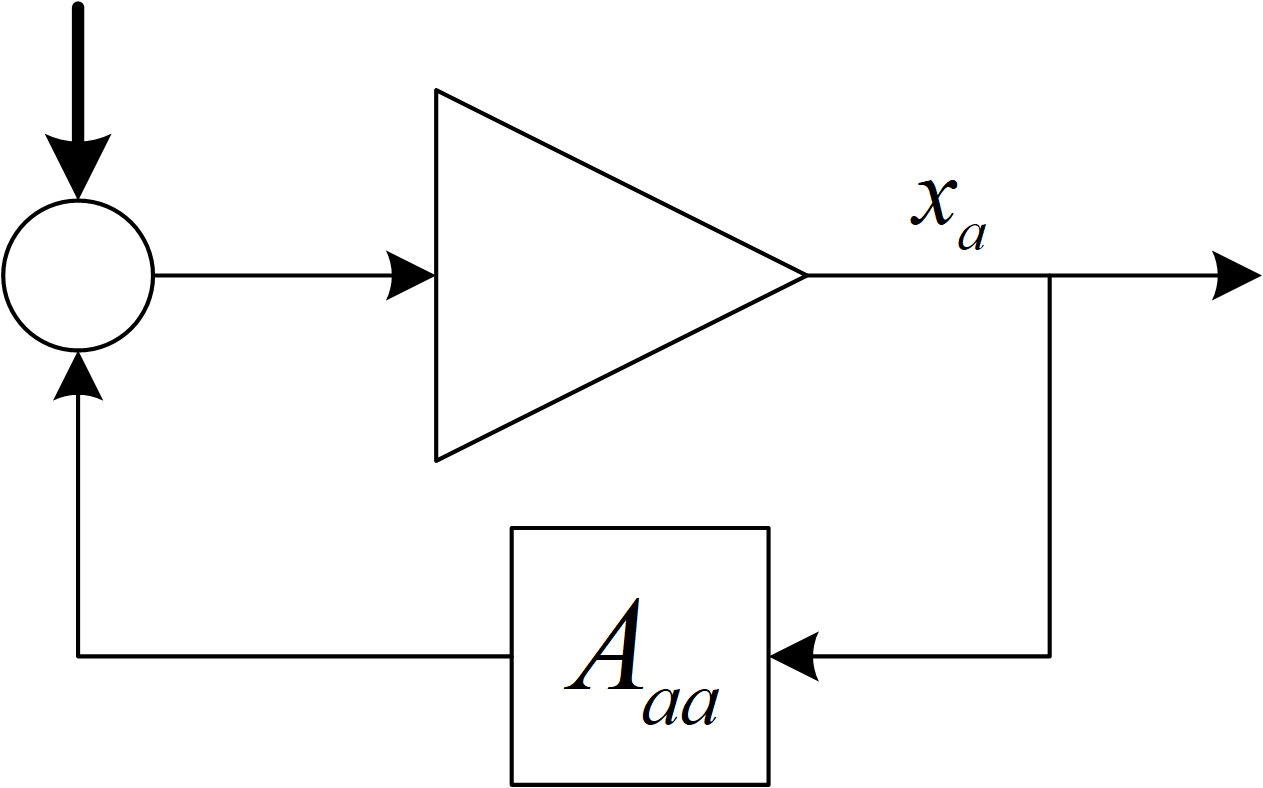
\includegraphics[scale=1]{xa.png}} \\
	\subfigure[$x_{b,\iota}$ the chain of integrators without a direct input.]{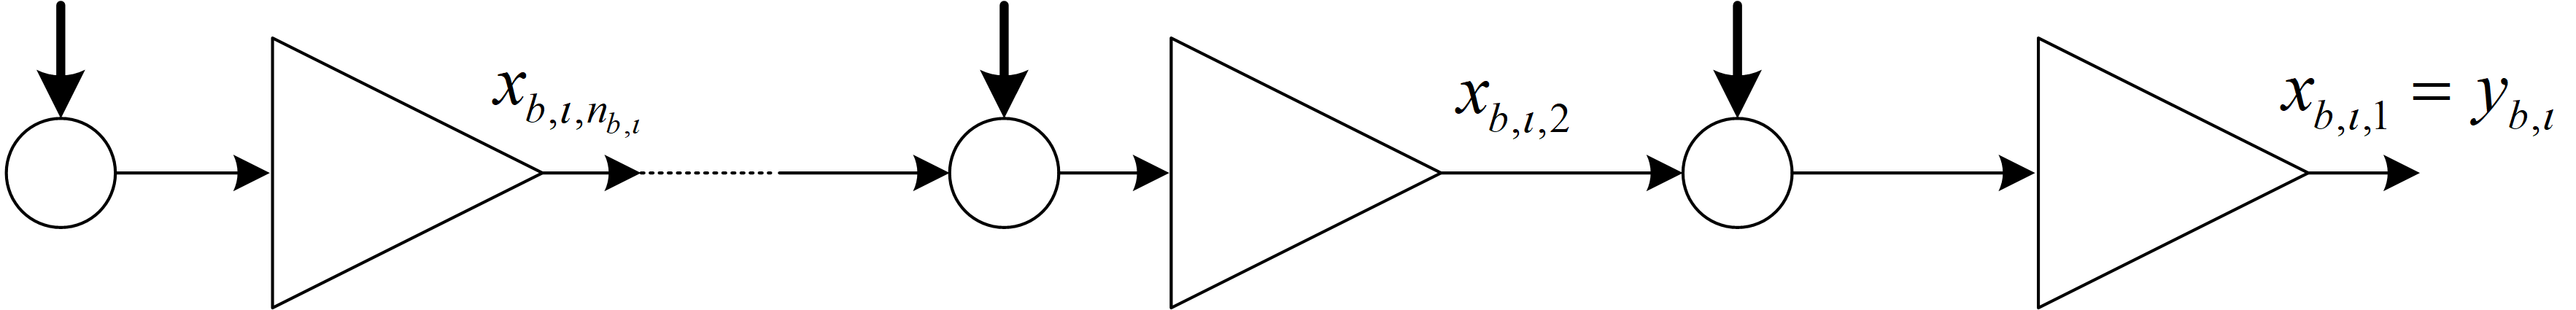
\includegraphics[scale=1]{xb.png}} \\
	\subfigure[$x_{c,k}$ the chain of integrators without a direct output.]{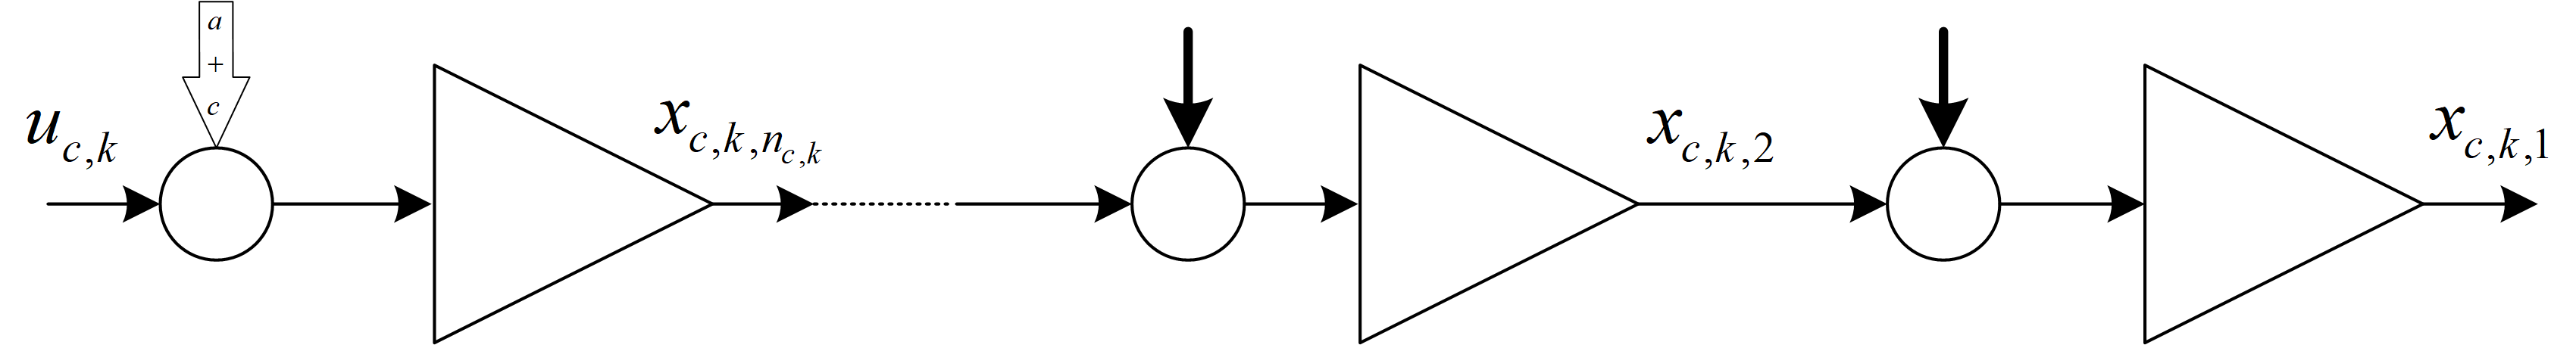
\includegraphics[scale=1]{xc.png}} \\
	\subfigure[$x_{d,i}$ the chain of integrators with direct input and output.]{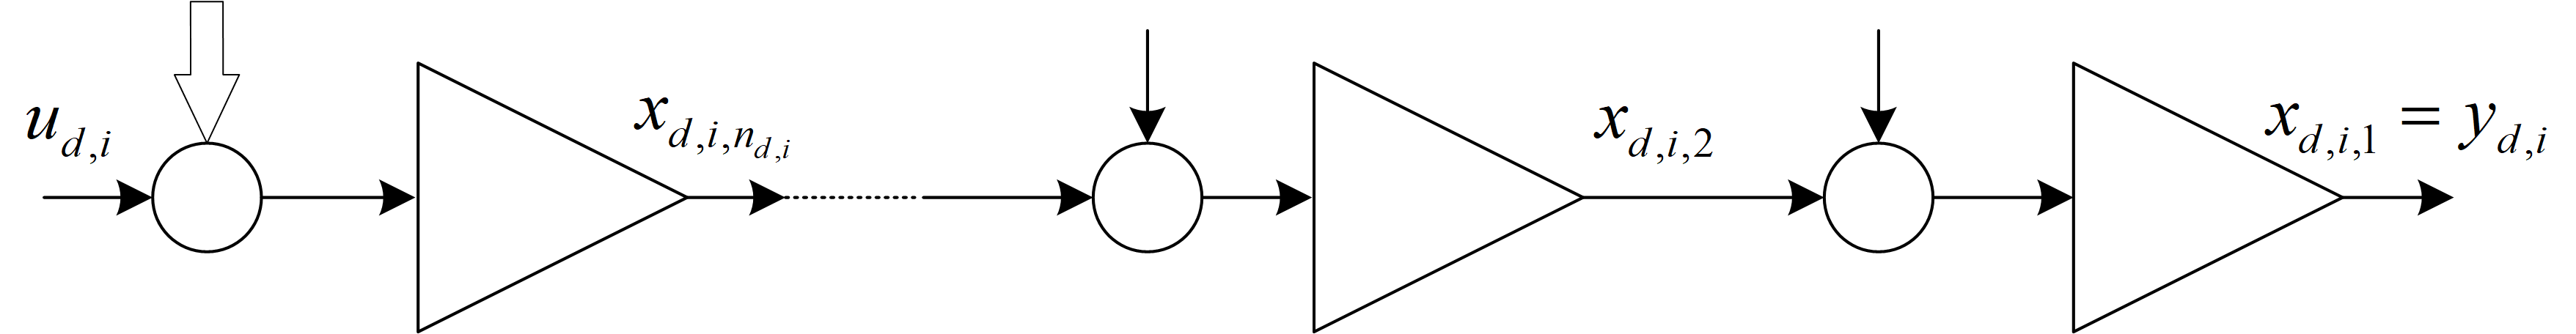
\includegraphics[scale=1]{xd.png}}
	\caption{Graphic interpretation of structural SCB decomposition of a MIMO system.}
	\label{fig: SCB}
\end{figure}

The proof of this Theorem \ref*{theorem: SCB} is given in \cite{Chen2004}. For simplicity, the system \eqref{ecu: Sigma} is considered without feedthrough (the arguments in following chapters are equally applicable with an extra steps in SCB transformation). Although the procedure for the decomposition of MIMO systems is complicated, the principal idea is the identification of chains of integrators between the system input and output variables. Three different types of chains of integrators can be identified:

\begin{enumerate}
	\item Chains that start from an input channel and end with an output. This type
	of chain gives the infinite zero structures of the given system and covers the
	subspace corresponding to $x_d$.
	\item Chains that start from an input channel but do not end with an output. This
	type of chain covers the subspace corresponding to $x_c$.
	\item Chains that do not start from an input but end with an output variable. This
	type of chain covers the subspace corresponding to $x_b$.
\end{enumerate}

These subspaces do not cover the whole state space of the given system. The remaining part forms a subspace corresponding to $x_a$, which is related to the invariant zeros of the system, i.e. the zeros dynamics. These four subsystems $x_a,x_b,x_c,x_d$ are depicted in graphical form in Figure \ref{fig: SCB}.



where the signal indicated by the double-edged arrow in $x_d$ is a linear combination of all the state variables; the signal indicated by the double-edged arrow marked with $a + c$ in $x_c$ is a linear combination of the state variables $x_a$ and $x_c$; the signals indicated by the thick vertical arrows are some linear combinations of the output variables $y_d$ and $y_b$; and the signals indicated by the thin vertical arrows are some linear combinations of the output variable $y_d$.

The subsystems have the following properties
\begin{enumerate}
	\item $\Sigma_a$ corresponds to the zeros dynamics. If $A_{aa}$ is Hurwitz then it is detectable. If not it is undetectable.
	\item Subsystem $\Sigma_b$ is not affected by the unknown input vector, and it is observable. Therefore it can be expressed in observer or observability canonical form. \eqref{ecu: xd} is expressed as the latter.
	\item Subsystem $\Sigma_c$ is affected by the unknown input, it is not strongly observable.
	\item Subsystem $\Sigma_d$ is affected by the unknown input vector, it is strongly observable, and because the number of inputs and outputs is the same $p_d$ then the subsystem is square.
\end{enumerate}

Several important properties of linear systems for this work can be displayed by the SCB, nonetheless, before that, some definitions about observability and detectability  for systems with unknown inputs have to be remembered.

\begin{definition}
	The zeros of the system \eqref{ecu: Sigma} correspond to the values $s\in \mathbb{C}$ for which the Rosenbrock's matrix 
	\begin{equation}\label{ecu: Rosenbrok}
		\begin{split}
			R(s)=
			\begin{bmatrix}
				sI-A & -D\\
				C & 0	
			\end{bmatrix}, \quad \forall s\in \mathbb{C}
		\end{split}
	\end{equation} 
	loses rank, i.e. $rank[R(s)] < n+m$.
\end{definition}

\begin{definition}
	The system \eqref{ecu: Sigma} is strongly observable if 
	\begin{equation}
		y(t)=0 \textup{ for } t>0  \quad \textup{ implies }  \quad x(t) = 0 (t > 0)
	\end{equation}
	for any input and initial state. \\
	Equivalently, the system is strongly observable if and only if it has no zeros.
\end{definition}

\begin{definition}
	The system \eqref{ecu: Sigma} is strongly detectable if 
	\begin{equation}
		y(t)=0 \textup{ for } t>0 \quad \textup{ implies }  \quad  x(t) \rightarrow 0 (t \rightarrow 0)
	\end{equation}
	for all inputs and initial states. \\
	Equivalently, the system is strongly detectable if and only if all its zeros $s$ satisfy $Re[s] < 0$.
\end{definition}
\newpage
\begin{definition}\label{def: Strong Det*}
	The system \eqref{ecu: Sigma} is strongly$^*$ detectable if 
	\begin{equation}
		y(t)\rightarrow 0 (t \rightarrow 0)  \quad  \textup{ implies }  \quad  x(t) \rightarrow 0 (t \rightarrow 0)
	\end{equation}
	for all inputs and initial states. \\
	Equivalently, the system is strongly$^*$ detectable if and only if it is strongly detectable, i.e.
	\begin{equation}\label{ecu: Fase minima}
		\begin{split}
			rank
			\begin{bmatrix}
				sI-A & -D\\
				C & 0	
			\end{bmatrix}=n+m, \quad \forall s\in \mathbb{C}
		\end{split}
	\end{equation}
	 and additionally
	\begin{equation}\label{ecu: Cond rel deg 1}
			rank(CD) = rank(D)
	\end{equation} 
\end{definition}

Consequently of these definitions strong observability implies strong detectability but it does not imply strong$^*$ detectability.

As mentioned before, all the invariant properties of the given system can be easily obtained from the structural decomposition. Then it can be now stated the next property of the system and subsystems in SCB coordinates.

\begin{property}
	The system $\Sigma_{SCB}$ in \eqref{ecu: Sigma SCB} is strong observable if and only if, $x_a$ and $x_c$ are non-existent.
\end{property}

\section{Conditions for the existence of Unknown Input Observers}
In \cite{Hautus1983}\cite{Trentelman2001} the necessary and sufficient conditions for the existence of observers for systems in which the input is not completely available for measurement were introduced, i.e. Observers with of Unknown Inputs (UIO) signals. Such conditions are described in terms of the properties before mentioned related to the structure of the system. 

\begin{theorem}
Under the assumption that the unknown input $\omega(t)$ is a completely arbitrary signal, e.g. it may be unbounded. The system $\Sigma$ in \eqref{ecu: Sigma} has a Unknown Input Observer if and only if it is Strong Detectable$^*$, i.e.

\end{theorem}

This, in Definition \ref{def: Strong Det*} is equivalent to have minimum phase condition, since the rank of the Rosenbrock matrix has to be equal to $n + m, \forall s\in \mathbb{C}$ or the absence of invariant zeros. And, from \eqref{ecu: Cond rel deg 1} a relative degree one condition. Based on the definition we can emphasize:

\begin{observation}
	Strong detectability or even strong observability is not sufficient for the existence of an Unknown Input Observer.
\end{observation}

Since the conditions of minimum phase and relative degree one are necessary and sufficient, it is impossible to overcome them without imposing another restrictions to the problem formulation. Hereafter the following is assumed

\begin{assumtion}
	The unknown input $\omega(t)$ is uniformly bounded, i.e. there exist some $\Delta \in \RE_{\geq 0}$ such that $\norm{\omega(t)}<\Delta$.
\end{assumtion}

\section{Homogeneity and Bl-homogeneity}
Homogeneity is the property whereby objects such as functions or vector fields scale in a consistent fashion with respect to a scaling operation called a dilation \cite{Bernuau2014}, which is essentially an action of the multiplicative group of positive real numbers on the state space \cite{Bhat2005}. Homogeneity with respect to the standard dilation is one of the two axioms for linearity, the other being additivity. Many familiar properties of linear systems follow, in fact, from homogeneity alone. The first step of homogeneity consists in homogeneous polynomials. The Euler’s homogeneous function theorem was the first result linking homogeneity with analysis. And in control theory, homogeneity appeared with Lasalle and Hahn in the 40’s. 

\begin{definition}
	Let $n$ and $m$ be two positive integers. A mapping $f: \RE^n \rightarrow \RE^m$ is said to be homogeneous (in the classical sense) with degree $l \in \RE$ if and only if $\forall \epsilon>0: \quad f(\epsilon x) = \epsilon^lf(x)$.
\end{definition}

The main issue with the classical homogeneity was its very restrictive field of use. Hence, a generalization of the classical homogeneity was proposed by V.I. Zubov in 50s and developed by H. Hermes in the 90’s using different weights, leading to weighted homogeneity. Nowadays, this is the most popular definition of homogeneity \cite{Bernuau2014}.

\begin{definition}
	Fix a set of coordinates $(x_1,...,x_n)\in \RE^n$. Let $\epsilon>0$ all real numbers and $r=(r_1,...,r_n)$ be a n-upled of positive real numbers. The dilation operator is defined as $\Delta_{\epsilon}^{r}x = \left[ \epsilon^{r_1}x_1,...,\epsilon^{r_n}x_n \right]^T$, where the numbers $r_i$ are the weights of the coordinates. The map also can be written as $\Delta_{\epsilon}^{r}x = diag(\epsilon^{r_1},...,\epsilon^{r_n})x$, where $\Delta_{\epsilon}^{r}$ is the dilation matrix and $x$ the vector of coordinates.
\end{definition}

\begin{definition}
	It is said that
	\begin{itemize} 
		\item A function $V: \RE^n \rightarrow \RE$ is $r$-homogeneous of degree $l$ or $(r,l)$-homogeneous for short, if the equality $V(\Delta_{\epsilon}^{r}x) = \epsilon^lV(x), \forall x\in \RE^n  \textbackslash \{0 \}, \forall \epsilon >0$ holds.
		\item A vector field $f: \RE^n \rightarrow \RE^n$ is $r$-homogeneous of degree $l$, if the equality $f(\Delta_{\epsilon}^{r}x) = \epsilon^l \Delta_{\epsilon}^{r} f(x), \forall x\in \RE^n  \textbackslash \{0 \}, \forall \epsilon >0$ holds.
		\item A vector-set field $F: \RE^n \rightrightarrows\RE^n$, $F(x), \subset \RE^n$ is $r$-homogeneous of degree $l$, if the equality $F(\Delta_{\epsilon}^{r}x) = \epsilon^l \Delta_{\epsilon}^{r} F(x), \forall x\in \RE^n  \textbackslash \{0 \}, \forall \epsilon >0$ holds.
		\item A system $\dot{x} = f(x)$ is homogeneous if and only if $f$ is so.
	\end{itemize}
\end{definition}

An extension to this concept has is the homogeneity in the bi-limit or bl-homogeneity for short.

\begin{definition}
	A function $\varphi: \RE^n \rightarrow \RE$ is said to be homogeneous in the $0$-limit with associated triple $(r_0,l_0,\varphi_0)$, if it is approximated near $x=0$ by the $(r_0,l_0)$-homogeneous function $\varphi_0$. It is said to be homogeneous in the $\infty$-limit with associated triple $(r_{\infty},l_{\infty},\varphi_{\infty})$, if it is approximated near $x=\infty$ by the $(r_{\infty},l_{\infty})$-homogeneous function $\varphi_{\infty}$. Similar definitions apply for vector fields and set-valued vector fields.
	
	Consequently, a function $\varphi: \RE^n \rightarrow \RE$ (or a vector field or set-valued vector field) is said to be homogeneous in the bi-limit if it is homogeneous in the $0$-limit and homogeneous in the $\infty$-limit.
\end{definition}

There are several results related to the homogeneity of functions, which are going to be useful for the stability analysis in the following chapters. Here we recall some of them. Fisrstly, let us mention that the regularity of a homogeneous mapping $f$ is related to its degree:

\begin{theorem}\label{theo: Regularity}
	Suppose $f: \RE^n \rightarrow \RE$ is continuous on $\RE^n \textbackslash \{0 \}$ and homogeneous of degree $l$. Then
	\begin{itemize}
		\item If $l<0$, the $f$ is continuous on $\RE^n$ if and only if $V\equiv 0$.
		\item If $l=0$, the $f$ is continuous on $\RE^n$ if and only if $V\equiv V(0)$.
		\item If $l>0$, the $f$ is continuous on $\RE^n$.
	\end{itemize}
\end{theorem}
The proof of this Theorem \ref{theo: Regularity} is given in \cite{Bhat2005}. 

The following lemma asserts that sign-definite, homogeneous functions are radially unbounded.

\begin{lemma}
	Suppose $V: \RE^n \rightarrow \RE$ is continuous and homogeneous, then
	\begin{itemize}
		\item If $V$ is sign definite, then $V$ is radially unbounded.
		\item If $n>1$ and $V$ is proper, then $V$ is sign definite.
	\end{itemize}
\end{lemma}

This property is useful in the task of Lyapunov functions construction. Another useful result, but in bl-homogeneous functions, which going to be used in the proof of main result is as follows.

\begin{lemma}
	Let $\gamma: \RE^n \rightarrow \RE$ and  $\eta: \RE^n \rightarrow \RE_{\leq 0}$ be two upper semicontinuous (u.s.c.) single-valued bl-homogeneous functions, with the same weights $r_0$ and $r_1$, degrees $m_0$ and $m_{\infty}$, and approximating functions $\eta_{0},\eta_{\infty}$ and $\gamma_0,\gamma_{\infty}$ which are u.s.c. Suppose that $\forall x\in\RE^n$, $\gamma(x)\leq 0$, $\gamma_0(x)\leq 0$, $\gamma_{\infty}(x)\leq 0$. If $\gamma(x)=0 \wedge x\neq 0 \Rightarrow \eta(x)<0$, $\gamma_{\iota}(x)=0 \wedge x\neq 0 \Rightarrow \eta_{\iota}(x)<0$ for $\iota \in \{0,\infty\}$, then there are constants $\lambda^*\in\RE$, $c_0>0,c_{\infty}>0$ such that for all $\lambda \geq max\{\lambda_0,\lambda_{\infty}\}, \lambda_0 \geq \lambda^*$, $\lambda_{\infty}>\lambda^*$ and for all $x\in \RE^n \textbackslash \{0 \}$,
	\begin{equation}
		\begin{split}
		\eta(x)+\lambda\gamma(x) \leq -c_0\norm{x}_{r_0,p}^{m_0} - c_{\infty}\norm{x}_{r_{\infty},p}^{m_{\infty}}, \\
		\eta_{\iota}(x)+\lambda\gamma_{\iota}(x) \leq -c_{\iota}\norm{x}_{r_{\iota},p}^{m_{\iota}}, \quad \iota \in \{0,\infty\}
		\end{split}
	\end{equation}
\end{lemma}


\subsection{Stability of homogeneous systems}
There are some crucial stability results that appear in the literature for the special case of systems that are homogeneous with respect to dilations of the form  $\Delta_{\epsilon}^{r}x$. But before presenting them, we formalize the concepts of stability, and the classical results in Lyapunov stability will be remembered.

\begin{definition}
	Consider the autonomous system 
	\begin{equation}\label{ecu: sys Lyap}
		\dot{x}=f(x)
	\end{equation}
	whit $f: \RE^n \rightarrow \RE^n$. Then \\
	The equilibrium point $x=0$ of \eqref{ecu: sys Lyap} is 
	\begin{itemize}
		\item Stable if, for each $\epsilon>0$, there is $\delta=\delta(\epsilon)>$0 such that 
		\begin{equation}
			\norm{x(0)} < \delta \Rightarrow \norm{x(t)}<\epsilon, \forall t\geq 0
		\end{equation}
		\item Unstable if it is not stable.
		\item Asymptotically stable if it is stable  and $\delta$ can be chosen such that
		\begin{equation}
			\norm{x(0)} < \delta \Rightarrow \lim_{t\to \infty} x(t)=0
		\end{equation}
	\end{itemize}
\end{definition}

The well known Lyapunov's stability theorem is as follows, taken from \cite{Khalil2003}

\begin{theorem}
	Let $x=0$ be an equilibrium point for \eqref{ecu: sys Lyap} and $D\subset \RE^n$ be a domain containing $x=0$. Let $V: D\rightarrow \RE$ be a continuously differentiable function such that
	\begin{equation}
		\begin{split}
		V(0) = 0 \quad and \quad V(x) &> 0 \quad in \quad D \textbackslash \{0 \} \\
		\dot{V}(x) &\leq 0 \quad in \quad D
		\end{split}
	\end{equation}
	Then, $x=0$ is stable. Moreover, if 
	\begin{equation}
		\dot{V}(x) < 0 \quad in \quad D \textbackslash \{0 \}
	\end{equation}
	then, $x=0$ is asymptotically stable.
\end{theorem}

This is local result, which can be extended to globally stability as shown in the next theorem

\begin{theorem}
		Let $x=0$ be an equilibrium point for \eqref{ecu: sys Lyap}. Let $V: \RE^n \rightarrow \RE^n$ be a continuously differentiable function such that
	\begin{equation}
			V(0) = 0 \quad and \quad V(x) > 0 \quad \forall x \neq 0 \\
	\end{equation}
	$V$ is radially unbounded, i.e.
	\begin{equation}
		\norm{x} \rightarrow \infty \Rightarrow V(x) \rightarrow \infty
	\end{equation}
	and
	\begin{equation}
		\dot{V}(x) < 0 \quad \forall x\neq 0
	\end{equation}
	then, $x=0$ is globally asymptotically stable.
\end{theorem} 

Before giving some results related to homogeneous systems, we will recall a few definitions about stability in some stronger sense. 

\begin{definition}
	\cite{Bhat2005} The system \eqref{ecu: sys Lyap} is said to be finite-time stable (FTS) at the origin (on an open neighborhood $\mathcal{V} \subset \RE^n$ of the origin) if:
	\begin{itemize}
		\item There exists a funtion $\delta\in \mathcal{K}$ such that for all $x_0\in \mathcal{V}$ we have $\norm{(x_0)}\leq \delta(\norm{x_0})$ for all $t\geq 0$.
		\item There exists a function $T:\mathcal{V}\textbackslash \{0 \} \rightarrow \RE_{+}$ such that for all $x_0\in \mathcal{V}\textbackslash \{0 \}$, $x(x_0)$ is defined, unique, nonzero on $[0,T(x_0))$ and $\lim_{t\rightarrow T(x0)}x(x_0) = 0$. $T:\RE^n \rightarrow \RE_{+} \cup \{0\}$ is the settling-time function.
	\end{itemize}
	If $\mathcal{V}=\RE^n$, the the system is called globally FTS.
	
	For differential inclusions (DI) the notion has been defined to deals with all solutions originated from a given initial condition. Details can be seen in the reference.
\end{definition}

Finally, the fixed-time (FxT) stability is a particular case of the FTS property.

\begin{definition}
	The system \eqref{ecu: sys Lyap} is said to be FxT stable at the origin if it is globally FTS and the settling-time function $T$ is bounded, i.e. $\exists \bar{T}>0$ such that $T(x)<\bar{T}$ for all $x\in \RE^n$.
\end{definition}

\subsection{Homogeneous Lyapunov functions}
Now we are completely ready to set down the some principal implications about stability for homogeneous and bl-homogeneous systems, these are important because the observer construction in the next chapter keeps this properties, which will be useful in the mathematical proofs of stability and convergence. 

\begin{theorem}
	Let \eqref{ecu: sys Lyap} be a homogeneous system, if the origin a locally stable equilibrium point, then the origin os globally asymptotically stable.
\end{theorem}

It is well known that an Asymptotically Stable linear system possesses a strict Lyapunov function which is a quadratic form. It turns out that any homogeneous Asymptotically Stable system admits a homogeneous strict Lyapunov function, not necessarily quadratic. The following theorem formalize the existence of a Lyapunov function for a homogeneous system

\begin{theorem}\label{theo: Hom V}
	\cite{BacciottiAndRosier2005} Let $f$ a continuous vector field on $\RE^n$ such that the origin is a locally asymptotically stable equilibrium point. Assume that $f$ is $r$-homogeneous of degree $m$ with $r \in (0,+\infty)^n$. Then, for any $k\in \mathbb{N}$ and any $p > k\cdot max_i\{r_i\}$, there exists a strict Lyapunov function $V$ for the system \eqref{ecu: sys Lyap}, which is $r$-homogeneous of degree $p$ and of class $\mathcal{C}^k$. As a direct  consequence, the time derivative $V=\langle \nabla V,f \rangle$ is $r$-homogeneous of degree $m+p$.
\end{theorem} 

The following corollary shows that the rate convergence of trajectories for homogeneous asymptotically stable system is completely characterized by the degree of the field.

\begin{corollary}
	Let $f$ be as in \ref{theo: Hom V}, and let $\norm{\cdot}_{r,p}$ be any $r$-homogeneous norm.
	\begin{itemize}
		\item If $k<0$, then the origin is finite-time stable.
	\end{itemize}
\end{corollary}

There are some important points 
\begin{observation}\label{obs: Sys Homogeneous}
	In homogeneous systems we have that
\begin{itemize}
	\item Finite Time Stability (FTS) is equivalent to an infinite eigenvalue assignation for the closed-loop system at the origin, therefore the right-hand side of the ordinary differential equation cannot be locally Lipschitz at the origin.
	\item There exists the settling time function $T(x_0)$ that determines the time for a solution to reach the equilibrium, this function depends on the initial condition of a solution. In general this function $T$ can grow unboundedly (possibly more than linearly).
\end{itemize}
\end{observation}

The main issue with $T$ is its continuity at the origin. For continuous systems, the continuity of $T$ at $0$ is equivalent to the continuity of $T$ everywhere. The bi-limit homogeneity application allows us to have a globally bounded $T$, which means that in practice one gets a FxT convergence to the origin for all initial conditions.

A recently application of bl-homogeneity to the observation problem is in the differentiators development with correction terms having the property of being homogeneous in the bi-limit, therefore, under some assumptions of uniform bounding the observer is able to estimate exactly in FxT the true derivatives of a signal $f$. In fact, these results are closely linked to this work. More details will be given immediately.

\newpage
\section{Arbitrary Order Fixed-Time Differentiators}
\cite{Moreno2021} Given a signal $f(t)$ defined on $[0,\infty)$, the objective is to estimate some of its time derivatives. $f(t)$ is composed of a base signal $f_0$ n-times differentiable, and a uniformly bounded noise $v(t)$, i.e.$f(t)=f_0(t)+v(t)$ and $|f_0^{(n)}(t)|\leq \Delta$ with $\Delta \geq 0$.

Defining the variables $\varsigma_1=f_0(t), \varsigma_2=\dot{f}_0(t), .... ,\varsigma_n=f_0^{(n-1)}(t)$, where $f_0^{(i)}(t)=\frac{d^i}{dt^i}f_0(t)$. A state representation of $f_0$ is
\begin{equation}
	\begin{split}
		\dot{\varsigma}_i &= \varsigma_{i+1} \qquad i=1,...,n-1 \\
		\dot{\varsigma}_n &= f_0^{(n)}(t)
	\end{split}
\end{equation}

In order to estimate the derivatives $f_0^{(i)}(t)$ for $i=1,...,n-1$ we have the following nonlinear family of differentiators
\begin{equation}\label{ecu: dif Mor}
	\begin{split}
	\dot{x}_i &= -k_i\phi_i(x_1-y)+x_{i+1}, \qquad i=1,...,n-1 \\
	\dot{x}_n &= -k_n\phi_n(x_1-y)
	\end{split}
\end{equation}
where the nonlinear output injection terms, given by
\begin{equation}
	\phi_i(z) = \varphi_i \circ ...\varphi_2 \circ \varphi_1(z)
\end{equation} 
are the composition of the monotonic growing functions
\begin{equation}\label{ecu: varphi}
	\varphi_i(s) = \kappa_i \lceil s \rfloor^{\frac{r_{0,i+1}}{r_{0,i}}} + \theta_i \lceil s \rfloor^{\frac{r_{\infty,i+1}}{r_{\infty,i}}} 
\end{equation}
with powers selected as $r_{0,n}=r_{\infty,n}=1$, and for $i=1,...,n+1$
\begin{equation}
	\begin{split}
	r_{0,i} = r_{0,i+1}-d_0 = 1-(n-i)d_0 \\
	r_{\infty,i} = r_{\infty,i+1}-d_\infty = 1-(n-i)d_\infty
	\end{split}
\end{equation}
which are completely defined by two parameters $-1 \leq d_0 \leq d_\infty < \frac{1}{n-1}$. With this selection the first term in \eqref{ecu: varphi} is dominating for small values of $s$, while the second one is dominating for large values of $s$.

Differentiator (\ref{ecu: dif Mor}) is not homogeneous, but it is homogeneous in the bi-limit, that is, near to the origin it is approximated by a homogeneous system of degree $d_0$ and far from the origin it is approximated by a homogeneous system of degree $d_\infty$. Although the scaling properties of the homogeneous systems are lost, the design of bl-homogeneous differentiators is more flexible, since the properties near the origin and far from it can be assigned independently.

If we select $d_0 = d_1 = d$ the differentiator \eqref{ecu: dif Mor} becomes homogeneous. And making $d = 0$ it is obtained the High-Gain differentiator, for $d = -1$ Levant’s robust and exact differentiator is recovered and for other values of $d$ the family of continuous differentiators in \cite{CruzZavala2016}\cite{Sanchez2018}\cite{CruzZavala2019}\cite{Jbara2021} is attained. For polynomial signals note that if $d < 0$ (resp. $d = 0$) the estimation converges in finite-time (resp. exponentially). For $d > 0$ the convergence is asymptotic, but it attains any neighborhood of zero in a time which is uniform in the initial conditions.

A particular case of interest for the differentiator is a property that is only achieved when $d0 = -1$. In that case $\phi_n$ is discontinuous and it induces a Higher-Order Sliding-Mode at the origin, allowing the estimation to converge (in the absence of noise) exactly, robustly and in finite-time to the real values of the signal derivatives when the $n$-th derivative of the signal is bounded by a non zero constant $\Delta \in \RE_{\geq 0}$, i.e. $|f_0^{(n)}(t)|\leq \Delta$. For all other values of $d_0 > -1$, the convergence is only achieved if $\Delta=0$.

As we mentioned in \ref{obs: Sys Homogeneous}, one of the disadvantages in homogeneous (including Levant’s exact) differentiators with $d_0 < 0$, is that the convergence time, although finite, grows unboundedly (and faster than linearly) with the size of the initial estimation error. One of the nice features of the bl-homogeneous design in general and of the proposed differentiator \eqref{ecu: dif Mor} in particular, is that assigning a positive homogeneity degree to the $\infty$-limit approximation $d_{\infty} > 0$ and a negative homogeneity degree to the $0$-limit approximation $d_0 < 0$, it is possible to counteract this effect: Convergence of the estimation will be achieved in Fixed-Time \cite{Moreno2021}.

The main result of this differentiators \eqref{ecu: dif Mor} can be expressed formally as follows. In the absence of noise, it is able to estimate asymptotically the first $n-1$ derivatives of the signal $f_0(t)$. Let $\mathscr{F}^{n}_{0} \triangleq \left\lbrace f^{(n)}(t) \equiv 0 \right\rbrace$ represent the class of polynomial signals and $\mathscr{F}^{n}_{\Delta} \triangleq \left\lbrace \left| f^{(n)}(t)\right| \leq \Delta \right\rbrace$ corresponds to the class of $n$-Lipschitz signals.

\begin{assumtion}\label{asump: blh differentiator}
	$f(t)=f_0(t)+\nu(t)$, with $f_0(t)$ $n-$times differentiable, $|f^{(n)}(t)|\leq \Delta$, and $\nu(t)$ a uniformly bounded measurable signal.
\end{assumtion}
Then it is possible to have the following statement

\begin{theorem}\label{theo: est diff blh}
	\cite{Moreno2021} Let the function $f(t)=f_0(t)$ be such that Assumption \ref{asump: blh differentiator} is fulfilled. Select $-1 \leq d_0 \leq d_\infty < \frac{1}{n-1}$ and choose arbitrary positive (internal) gains $\kappa_i>0$ and $\theta_i>0$, for $i=1,...,n$. Suppose that either $\Delta=0$ or $d_0=-1$. Under this conditions, and in the absence of noise ($\nu(t) \equiv 0$) there exist appropriate gains $k_i>0$, for $i=1,...,n$, such that the solutions bl-homogeneous differentiator \eqref{ecu: dif Mor} converge globally and asymptotically to the derivatives of signal, i.e. $x_i(t) \rightarrow f_0^{(i-1)}(t)$ as $t \rightarrow \infty$. In particular, they converge in Fixed-Time, i.e. $\exists \bar{T}>0$ such that for any $x_i(0) \in \mathbb{R}^n$, $x_i(t) \equiv f_0^{(i-1)}(t)$ for $t \geq \bar{T}$ for $i=1,...,n$ if either
	\begin{eqnarray*}
		&(a)& \quad -1 < d_0 < 0 < d_\infty < \frac{1}{n-1} \quad and \quad f(t)\in \mathscr{F}^{n}_{0},  \quad or \\
		&(b)& \quad -1 = d_0 < 0 < d_\infty < \frac{1}{n-1} \quad and \quad f(t)\in \mathscr{F}^{n}_{\Delta}.
	\end{eqnarray*}
\end{theorem}

The proof of this Theorem \ref{theo: est diff blh}, which is of essential importance in this work is given in the the Apendix A and detailed in \cite{Moreno2021}.

This differentiator can be seen as an observer for a special type of SISO systems, composed by a chain of $n$ integrators and with a unknown input. The idea of this work is generalizing this observer to a family of MIMO-LTI systems by decomposing the original system in a set of subsystems and designing a bl-homogeneous observer composed by a set of sub-observers with unknown inputs. And proof that the convergence is achieved exactly and in fixed time by appropriately selecting the set of gains in the observer. 

With the necessary theory of homogeneous and bl-homogeneous systems given in this chapter, we are ready to present the main contribution of this work in Chapter 3.



%Observer
%It is important to note that observer (17)-(19) is not a simple use of a HOSM differentiator, replacing the ideal derivatives in observer (16), but it is an observer, with discontinuous injection terms.





	%====================================================================
	%                          Bibliografia
	%====================================================================
	\bibliographystyle{ieeetr} 
	\bibliography{Citas}
\end{document}
\chapter{Calculo de ganancias para controladoers discontinuos homogeneos de grado cero} \label{Cap3}
\section{Controlador de primer orden}
Sea el sitema \ref{eq:modelo1} afin a la entrada, de grado relativo 1, 
\begin{subequations}\label{eq:modelo1}
  \begin{align}\label{eq:modelo1a}
    \dot{x}_1&=f(x) +u 
  \end{align}
\end{subequations}
Con el algoritmo de control discontinuo
  \begin{equation}
      u=-k_1 \left\lceil x_1  \right\rfloor^0
    \end{equation} 

    Función de Lyapunov de control
    \begin{equation}
          V_1=\gamma_1 \frac{r_1}{m} |x_1|^{\frac{m}{r_1}}
    \end{equation}
%%%%%%%%%%%%%%%%%%%%%%%%%%%%%%%%%%%%%%%%%%%%%%%%%%%%%%%5
%%%%5
%%%%%%%%%%%%%%%%%%%%%%%%%%%%%%%%%%%%%%%%%%%%%%%%%%%%%%%%%%
\section{Controlador de segundo orden}
Sea el sitema \ref{eq:modelo2} afin a la entrada, de grado relativo 2, 
\begin{subequations}\label{eq:modelo2}
  \begin{align}\label{eq:modelo1a}
    \dot{x}_1&=x_2 \\
    \dot{x}_2&=u
  \end{align}
\end{subequations}


  \begin{equation}
      \begin{split}
      \dot{x}_1&=x_2\\
      \dot{x}_2& \in [-C,C]+ [k_m, k_M] u
      \end{split}
      \label{inclusion2}
  \end{equation}
  Con el algoritmo de control discontinuo anidado
  \begin{equation}
      u=-k_2 \left\lceil \lceil x_2 \rfloor^{\alpha_2}+k_1^{\alpha_2} \lceil x_1 \rfloor^{\frac{\alpha_2}{2}} \right\rfloor^0
    \end{equation} 
    Función de Lyapunov de control
  \begin{equation}
        V_2=\gamma_1 \frac{r_1}{m} |x_1|^{\frac{m}{r_1}}+\frac{r_2}{m} |x_2|^{\frac{m}{r_2}}-\lceil \upsilon_1 \rfloor^{\frac{m-r_2}{r_2}} x_2 + \left(1-\frac{r_2}{m}\right)|\upsilon_1|^{\frac{m}{r_2}}
  \end{equation}
  \begin{equation}
        \upsilon_1=-k_1 \lceil x_1 \rfloor^{\frac{r_2}{r_1}}
   \end{equation}

   donde 
   \begin{equation}
        W_2 = \frac{r_2}{m} |x_2|^{\frac{m}{r_2}} - \lceil \upsilon_1 \rfloor^{\frac{m-r_2}{r_2}} x_2 + (1+\frac{r_2}{m})|\upsilon_1|^{\frac{m}{r_2}}
   \end{equation} 

   
   \begin{equation}
        \begin{split}
             \frac{\partial W_2}{\partial x_1}&=-\frac{m-r_2}{r_2} x_2 |\upsilon_1|^{\frac{m-2r_2}{r_2}} \frac{\partial \upsilon_1}{\partial x_1}+\frac{m-r_2}{r_2}\lceil \upsilon_1 \rfloor^{\frac{m-r_2}{r_2}}\frac{\partial \upsilon_1}{\partial x_1}\\
             &\textbf{sustituimos $x_2=s_2+\upsilon_1$} \\
             &=\frac{m-r_2}{r_2} \frac{\partial \upsilon_1}{\partial x_1} \left( -|\upsilon_1|^{\frac{m-2r_2}{r_2}}s_2 -\lceil \upsilon_1 \rfloor^{\frac{m-r_2}{r_2}} +\lceil \upsilon_1 \rfloor^{\frac{m-r_2}{r_2}} \right)\\
             &=-\frac{m-r_2}{r_2} \frac{\partial \upsilon_1}{\partial x_1} \left( |\upsilon_1|^{\frac{m-2r_2}{r_2}}s_2 \right)
        \end{split}
   \end{equation}

   donde
   \begin{equation}
       \upsilon_1=-k_1\lceil \sigma_1 \rfloor^{\frac{r_2}{\alpha_1}}=-k_1\lceil x_1 \rfloor^{\frac{r_2}{r_1}}
   \end{equation}
   \begin{equation}
       \frac{\partial \upsilon_1}{\partial x_1}= -k_1 \frac{r_2}{\alpha_1} |\sigma_1|^{\frac{r_2-\alpha_1}{\alpha_1}} \frac{\partial \sigma_1}{\partial x_1}  = -k_1 \frac{r_2}{r_1}|x_1|^{\frac{r_2-r_1}{r_1}}
   \end{equation}
   \begin{equation}
     \sigma_1=\lceil x_1 \rfloor^{\frac{\alpha_1}{r_1}}
   \end{equation}
   \begin{equation}
     \frac{\partial \sigma_1}{\partial x_1}=\frac{\alpha_1}{r_1} |x_1|^{\frac{\alpha_1-r_1}{r_1}}
   \end{equation}
   para llegar a la ecuacion del articulo tenemos
   \begin{equation}
     \frac{\partial \upsilon_1}{\partial x_1}= -k_1 \frac{r_2}{\alpha_1} |\sigma_1|^{\frac{r_2-\alpha_1}{\alpha_1}} \frac{\partial \sigma_1}{\partial x_1}= -k_1 \frac{r_2}{\alpha_1} \textcolor{red}{\frac{k_1^{\frac{r_2-\alpha_1}{r_2}}}{k_1^{\frac{r_2-\alpha_1}{r_2}}}}  |\sigma_1 |^{\textcolor{red}{\frac{r_2}{r_2}} \frac{r_2-\alpha_1}{\alpha_1}} \frac{\partial \sigma_1}{\partial x_1}
 \end{equation}
 \begin{equation}
   |\upsilon_1|^{\frac{r_2-\alpha_1}{r_2}}=|-k_1\lceil \sigma_1 \rfloor^{\frac{r_2}{\alpha_1}}|^{\frac{r_2-\alpha_1}{r_2}}=k_1^{\frac{r_2-\alpha_1}{r_2}}|\lceil \sigma_1 \rfloor^{\frac{r_2}{\alpha_1}}|^{\frac{r_2-\alpha_1}{r_2}}=k_1^{\frac{r_2-\alpha_1}{r_2}}|\sigma_1|^{\frac{r_2-\alpha_1}{\alpha_1}}
 \end{equation}
 
 por lo que 
 \begin{equation}
   \frac{\partial \upsilon_1}{\partial x_1}= -k_1 \frac{r_2}{\alpha_1} \textcolor{red}{\frac{1}{k_1^{\frac{r_2-\alpha_1}{r_2}}}} |\upsilon_1|^{\frac{r_2-\alpha_1}{r_2}} \frac{\partial \sigma_1}{\partial x_1}= -\frac{r_2}{\alpha_1} k_1^{\frac{\alpha_1}{r_2}} |\upsilon_1|^{\frac{r_2-\alpha_1}{r_2}} \frac{\partial \sigma_1}{\partial x_1}
\end{equation}
obtenemos la parcial de nuevo sustituyendo la ecuacion antetior
\begin{equation}
 \begin{split}
      \frac{\partial W_2}{\partial x_1}&=-\frac{m-r_2}{r_2} \frac{\partial \upsilon_1}{\partial x_1} \left( |\upsilon_1|^{\frac{m-2r_2}{r_2}}s_2 \right)\\
      &=-\frac{m-r_2}{r_2} \left(  -\frac{r_2}{\alpha_1} k_1^{\frac{\alpha_1}{r_2}} |\upsilon_1|^{\frac{r_2-\alpha_1}{r_2}} \frac{\partial \sigma_1}{\partial x_1} \right) \left( |\upsilon_1|^{\frac{m-2r_2}{r_2}}s_2 \right)\\
      &=\frac{m-r_2}{\alpha_1} k_1^{\frac{\alpha_1}{r_2}}  |\upsilon_1|^{\frac{m-r_2-\alpha_1}{r_2}}  s_2 \frac{\partial \sigma_1}{\partial x_1} \\
 \end{split}
\end{equation}

obtenemos la forma explicita de la parcial con respecto a $x_1$ de $W_2$
\begin{equation}
  \begin{split}
       \frac{\partial W_2}{\partial x_1}&=\frac{m-r_2}{\alpha_1} k_1^{\frac{\alpha_1}{r_2}}  |\upsilon_1|^{\frac{m-r_2-\alpha_1}{r_2}}  s_2 \frac{\partial \sigma_1}{\partial x_1} \\
       &=\frac{m-r_2}{\alpha_1} k_1^{\frac{\alpha_1}{r_2}}  |\upsilon_1|^{\frac{m-r_2-\alpha_1}{r_2}}  \left(x_2 -\upsilon_1 \right) \left(\frac{\alpha_1}{r_1} |x_1|^{\frac{\alpha_1-r_1}{r_1}}\right) \\
       &=\frac{m-r_2}{r_1} k_1^{\frac{\alpha_1}{r_2}}  |-k_1\lceil x_1 \rfloor^{\frac{r_2}{r_1}}|^{\frac{m-r_2-\alpha_1}{r_2}}  \left(x_2 +k_1\lceil x_1 \rfloor^{\frac{r_2}{r_1}} \right) \left( |x_1|^{\frac{\alpha_1-r_1}{r_1}}\right) \\
       &=\frac{m-r_2}{r_1} k_1^{\frac{m-r_2}{r_2}}  | x_1|^{\frac{m-r_2-\alpha_1}{r_1}}  \left(x_2 +k_1\lceil x_1 \rfloor^{\frac{r_2}{r_1}} \right) \left( |x_1|^{\frac{\alpha_1-r_1}{r_1}}\right) \\
       &=\frac{m-r_2}{r_1} k_1^{\frac{m-r_2}{r_2}}  | x_1|^{\frac{m-r_2-r_1}{r_1}}  \left(x_2 +k_1\lceil x_1 \rfloor^{\frac{r_2}{r_1}} \right) \\
  \end{split}
\end{equation}
llegando asi  a la expresion del articulo con la diferencia de no tener signo negativo


   Llamaremos $f_2$ a la función a maximizar
   \begin{equation*}
     k_2> \frac{1}{k_m}\left( max\left[f_2 \right] + C \right)
   \end{equation*}
   \begin{equation}
     %\begin{split}
       f_2(\overline{x}_2) =  \frac{x_2\left(\gamma_1 \lceil x_1 \rfloor^{\frac{m-r_1}{r_1}} + \frac{m-r_2}{r_1} k_1^{\frac{m-r_2}{r_2}}  | x_1|^{\frac{m-r_2-r_1}{r_1}}  \left(x_2 +k_1\lceil x_1 \rfloor^{\frac{r_2}{r_1}} \right) \right)} {\left|\lceil x_2 \rfloor^{\frac{m-r_2}{r_2}}+k_1^{\frac{m-r_2}{r_2}}\lceil x_1 \rfloor^{\frac{m-r_2}{r_1}}\right|}= \frac{\phi_2}{|s_{2d}|}
     %\end{split}    
   \end{equation}

   \begin{equation}
    \begin{split}
      \frac{\partial f_2}{\partial x_1}- \frac{\partial f_2}{\partial x_2}&=|s_{2d}|\left( \frac{\partial \phi_2}{\partial x_1}-\frac{\partial \phi_2}{\partial x_2}\right) + \phi_2\left(\frac{\partial |s_{2d}|}{\partial x_2}-\frac{\partial |s_{2d}|}{\partial x_1}\right)\\
      &=|s_{2d}|\left( \frac{\partial \phi_2}{\partial x_1}-\frac{\partial \phi_2}{\partial x_2}\right) + \phi_2 \frac{s_{2d}}{|s_{2d}|}  \left(\frac{\partial s_{2d}}{\partial x_2}-\frac{\partial s_{2d}}{\partial x_1}\right)  \\
      &=\textcolor{red}{|s_{2d}|} \left(  |s_{2d}|\left( \frac{\partial \phi_2}{\partial x_1}-\frac{\partial \phi_2}{\partial x_2}\right) + \phi_2 \frac{s_{2d}}{|s_{2d}|}  \left(\frac{\partial s_{2d}}{\partial x_2}-\frac{\partial s_{2d}}{\partial x_1}\right)\right)  \\
      &= |s_{2d}|^2\left( \frac{\partial \phi_2}{\partial x_1}-\frac{\partial \phi_2}{\partial x_2}\right) + \phi_2 s_{2d}  \left(\frac{\partial s_{2d}}{\partial x_2}-\frac{\partial s_{2d}}{\partial x_1}\right) \\
      &=\textcolor{red}{s_{2d}} \left(  s_{2d}\left( \frac{\partial \phi_2}{\partial x_1}-\frac{\partial \phi_2}{\partial x_2}\right) + \phi_2  \left(\frac{\partial s_{2d}}{\partial x_2}-\frac{\partial s_{2d}}{\partial x_1}\right)\right)  \\
    \end{split}
  \end{equation}
  en la ultima ecuacion podemos observar que $s_{2d}$ es una solución; sin embargo, corresponde a los puntos donde se va a menos infinito por lo que son puntos minimos y los descartamos.
   
   Como la función es homogénea de grado cero, obtendremos un rayo de máximos con la siguiente forma:\\
      con $\textcolor{red}{x_1=1}$

      \begin{equation}
       \begin{split}
         M_p&:= max\left[f_2 \right]= \left(  \frac{\partial \phi_2}{\partial x_2} -  \frac{\frac{\partial \phi_2}{\partial x_1}}{\frac{\partial s_{2d}}{\partial x_1}}  \frac{\partial s_{2d}}{\partial x_2} \right) =c + d x_2 - \left( \frac{a}{e}  x_2 + \frac{b}{e} x_2^2 \right) f  |x_2|^{\frac{m-2r_2}{r_2}} \\
       \end{split}
     \end{equation}

     donde las constantes que dependen del valor de $k_1$
     \begin{equation}
       a=\gamma_1 \frac{m-r_1}{r_1} +\frac{m-r_2}{r_1} \frac{m-r_1}{r_1} k_1^{\frac{m}{r_2}}  
     \end{equation}
     \begin{equation}
       b=\frac{m-r_2}{r_1} \frac{m-r_2-r_1}{r_1} k_1^{\frac{m-r_2}{r_2}}
     \end{equation}
     \begin{equation}
       c=\gamma_1 +\frac{m-r_2}{r_1}k_1^{\frac{m}{r_2}}
     \end{equation}
     \begin{equation}
       d=2\frac{m-r_2}{r_1} k_1^{\frac{m-r_2}{r_2}}
     \end{equation}
     \begin{equation}
       e=\frac{m-r_2}{r_1} k_1^{\frac{m-r_2}{r_2}}
     \end{equation}
     \begin{equation}
       f=\frac{m-r_2}{r_2}
     \end{equation}

     Para encontrar el valor del máximo se debe obtener una raíz del rayo de máximos y evaluar el punto en la función a maximizar $f_2$

     \begin{equation*}
       max= f(1,x_2)
     \end{equation*}

     Sustituyendo con los valores del caso mas sencillo:
      $m=3$,$ y_1=k_1=1$, $r=[2,1]$

      \begin{equation*}
       a=1;\;\;\;b=0;\;\;\;c=2;\;\;\;d=2;\;\;\;e=1;\;\;\;f=2;
      \end{equation*}
      con $x_2>0$
     \begin{equation}
       M_p=2+2x_2-2x_2^2
     \end{equation}

     \begin{equation}
       \textcolor{red}{x_2=-0.618};  \;\;\;\;  x_2=1.618
     \end{equation}


     El máximo se obtine al evaluar en la función original:
     \begin{equation}
       max=f_2(1,1.618)=1.618
     \end{equation}

     Por lo tanto $k_2>1.618$

      \begin{figure}
        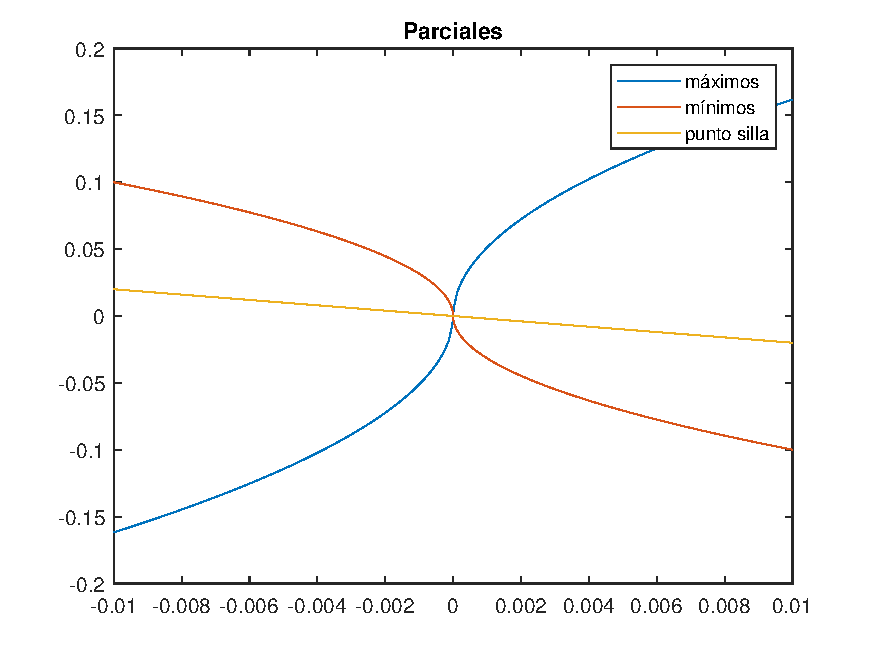
\includegraphics[width=0.49\textwidth,]{imagenes/grado2/rayos}
        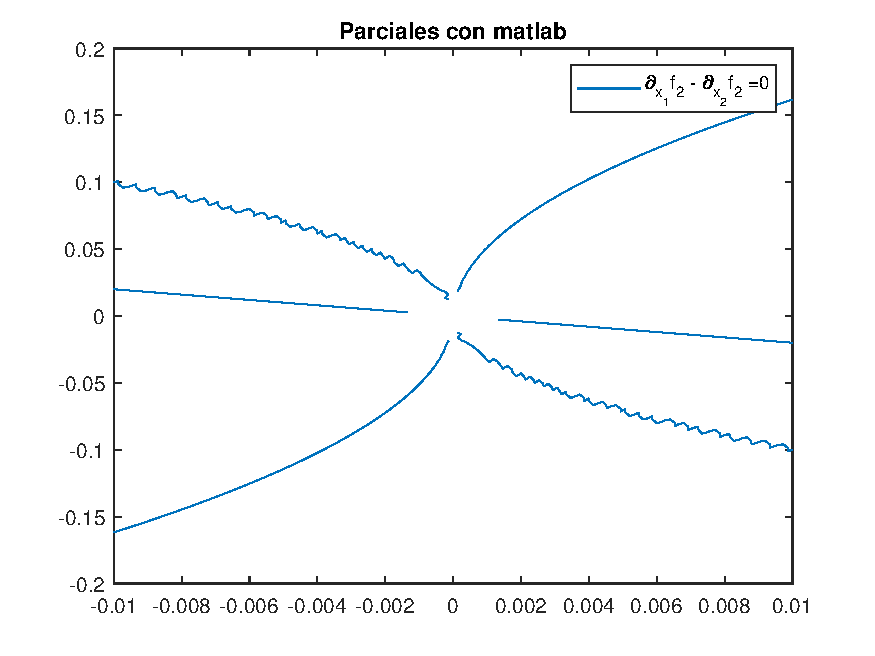
\includegraphics[width=0.49\textwidth,]{imagenes/grado2/parcialesMatalb.pdf}
        \caption{text}
        \label{text}
      \end{figure}
%%%%%%%%%%%%%%%%%%%%%%%%%%%%%%%%%%%%%%%%%%%%%%%%%%%%%%%%%%%%%%%%%%%%%%%%%%%%5
%%%%%%%%5      Grado 3
%%%%%%%%%%%%%%%%%%%%%%%%%%%%%%%%%%%%%%%%%5
\section{Para grado relativo 3}
Sea el sitema \ref{eq:modelo3} afin a la entrada, de grado relativo 3, 
\begin{subequations}\label{eq:modelo3}
  \begin{align}\label{eq:modelo1a}
    \dot{x}_1&=x_2 \\
    \dot{x}_2&=x_3 \\
    \dot{x}_3&=u
  \end{align}
\end{subequations}


  \begin{equation}
      \begin{split}
      \dot{x}_1&=x_2\\
      \dot{x}_2&=x_3\\
      \dot{x}_3& \in [-C,C]+ [k_m, k_M] u
      \end{split}
      \label{inclusion2}
  \end{equation}
  Con el algoritmo de control discontinuo anidado

    \begin{equation}
      u=-k_3 \left\lceil \lceil x_3 \rfloor^{\alpha_3}+k_2^{\alpha_3}\left\lceil \lceil x_2 \rfloor^{\frac{\alpha_2}{2}}+k_1^{\frac{\alpha_2}{2}} \lceil x_1 \rfloor^{\frac{\alpha_2}{3}}  \right\rfloor^{\frac{\alpha_3}{\alpha_2}} \right\rfloor^0
    \end{equation}
    
    Funcion de lyapunov de control
    \begin{equation}
      V_3=\gamma_2\left(\gamma_1 \frac{r_1}{m} |x_1|^{\frac{m}{r_1}}+\frac{r_2}{m} |x_2|^{\frac{m}{r_2}}-\lceil \upsilon_1 \rfloor^{\frac{m-r_2}{r_2}} x_2 + \left(1-\frac{r_2}{m}\right)|\upsilon_1|^{\frac{m}{r_2}}\right) +W_3
    \end{equation}

    La función a maximizar en su forma general:
    \begin{equation}
    k_2> max \left[ \frac{ \phi_2}{s_{2d} \lceil \sigma_2 \rfloor^{\frac{r_3}{\alpha_2}}} \right]:=max \left[ f_{32} \right]
  \end{equation}
Donde el rayo del máximo tiene la siguiente forma general:
  \begin{equation*}
    M:=\textcolor{red}{s_{2d} \frac{\partial \phi_2}{\partial x_1}- \phi_2 \left[ \frac{r_3}{\alpha_2} \frac{s_{2d} }{\sigma_2}  \frac{\partial \sigma_2}{\partial x_1} +  \frac{\partial s_{2d}}{\partial x_1}  \right]}
  \end{equation*}
Se fija $x_1=1$ y se busca una raiz para obtener el valor de $x_2$

\begin{equation}
  k_3> \frac{1}{k_m} max \left[  f_3 \right]+\frac{C}{k_m}:=\frac{1}{k_m}\frac{\phi_3}{|s_{3d}|}+\frac{C}{k_m}
\end{equation}
La función a obtener el máximo
\begin{equation}
  f_3:= \frac{\gamma_2 \gamma_1 x_2 s_{1d}   + \gamma_2  x_2  \frac{\partial W_2}{\partial x_1} + \gamma_2 x_3 \frac{\partial W_2}{\partial x_2}   + x_2 \frac{\partial W_3}{\partial x_1}  + x_3 \frac{\partial W_3}{\partial x_2}}{|s_{3d}|}
\end{equation}
Como la función es homogénea de grado cero, obtendremos un rayo de máximos con la siguiente forma:\\
con $\textcolor{red}{x_1=1, x_2=1}$
\begin{equation}
  \begin{split}
    max \left[  f_3 \right]=\frac{\partial \phi_3}{\partial x_3}- \frac{ \frac{\partial \phi_3}{\partial x_2}}{\frac{\partial s_{3d}}{\partial x_2}}\frac{\partial s_{3d}}{\partial x_3}=0\\
  \end{split}
\end{equation}



%%%%%%%%%%%%%%%%%%%%%%%%%%%%%%%%%%%%%%%%%%%%%%%%%%%%%%%%%%%%%%5
%%%          grado4
%%%%%%%%%%%%%%%%%%%%%%%%%%%%%%%%%%%%%%%%%%%%%%%%%%%%%%
\section{Para grado relativo 4}
Sea el sitema \ref{eq:modelo4} afin a la entrada, de grado relativo 4 , 
\begin{subequations}\label{eq:modelo4}
  \begin{align}\label{eq:modelo1a}
    \dot{x}_1&=x_2 \\
    \dot{x}_2&=x_3 \\
    \dot{x}_3&=x_4 \\
    \dot{x}_4&=u
  \end{align}
\end{subequations}


  \begin{equation}
      \begin{split}
      \dot{x}_1&=x_2\\
      \dot{x}_2&=x_3\\
      \dot{x}_3=x_4 \\
      \dot{x}_4& \in [-C,C]+ [k_m, k_M] u
      \end{split}
      \label{inclusion2}
  \end{equation}
  Con el algoritmo de control discontinuo anidado
  \begin{equation}
    u=-k_4 \left\lceil \lceil x_4 \rfloor^{\alpha_4}+ k_3^{\alpha_4} \left\lceil \lceil x_3 \rfloor^{\frac{\alpha_3}{2}}+k_2^{\frac{\alpha_3}{2}}\left\lceil \lceil x_2 \rfloor^{\frac{\alpha_2}{3}}+k_1^{\frac{\alpha_2}{3}} \lceil x_1 \rfloor^{\frac{\alpha_2}{4}}  \right\rfloor^{\frac{\alpha_3}{\alpha_2}} \right\rfloor^\frac{\alpha_3}{\alpha_2}\right\rfloor^0
  \end{equation}
  Función de Lyapunov de control
  \begin{equation}
    V_4=\gamma_3 V_3+W_4
  \end{equation}

  La función a maximizar en su forma general:
  \begin{equation}
  k_2> max \left[ \frac{ \phi_2}{s_{2d} \lceil \sigma_2 \rfloor^{\frac{r_3}{\alpha_2}}} \right]:=max \left[ f_{42} \right]
\end{equation}
Donde el rayo del máximo tiene la siguiente forma general:
\begin{equation*}
  M:=\textcolor{red}{s_{2d} \frac{\partial \phi_2}{\partial x_1}- \phi_2 \left[ \frac{r_3}{\alpha_2} \frac{s_{2d} }{\sigma_2}  \frac{\partial \sigma_2}{\partial x_1} +  \frac{\partial s_{2d}}{\partial x_1}  \right]}
\end{equation*}
Se fija $x_1=1$ y se busca una raiz para obtener el valor de $x_2$

La función a maximizar en su forma general:
\begin{equation}
k_3> max \left[ \frac{ \phi_3}{s_{3d} \lceil \sigma_3 \rfloor^{\frac{r_4}{\alpha_3}}} \right]:=max \left[ f_{43} \right]
\end{equation}
Donde el rayo del máximo tiene la siguiente forma general:
\begin{equation*}
M:=\textcolor{red}{s_{3d} \frac{\partial \phi_3}{\partial x_2}- \phi_3 \left[ \frac{r_4}{\alpha_3} \frac{s_{3d} }{\sigma_3}  \frac{\partial \sigma_3}{\partial x_2} +  \frac{\partial s_{3d}}{\partial x_2}  \right]}
\end{equation*}
Se fija $x_1=1, x_2=1$ y se busca una raiz para obtener el valor de $x_3$
\begin{equation}
  k_4> \frac{1}{k_m} max \left[  f_4 \right]+\frac{C}{k_m}:=\frac{1}{k_m}\frac{\phi_4}{|s_{4d}|}+\frac{C}{k_m}
\end{equation}
La función a obtener el máximo
\begin{equation}
  f_4:= \frac{ x_2 \frac{\partial V_4}{\partial x_1} + x_3 \frac{\partial V_4}{\partial x_2} + x_4 \frac{\partial V_4}{\partial x_3}  }{|s_{4d}|}
\end{equation}
Como la función es homogénea de grado cero, obtendremos un rayo de máximos con la siguiente forma:\\
con $\textcolor{red}{x_1=1, x_2=1, x_3=1}$
\begin{equation}
  \begin{split}
    max \left[  f_4 \right]=\frac{\partial \phi_4}{\partial x_4}- \frac{ \frac{\partial \phi_4}{\partial x_3}}{\frac{\partial s_{4d}}{\partial x_3}}\frac{\partial s_{4d}}{\partial x_4}=0\\
  \end{split}
\end{equation}

%%%%%%%%%%%%%%%%%%%%%%%%%%%%%%%%%%%%%%%%%%%%%%%%%%%%%%%%%%%%%%%%%%%%%%%%%%%%5
%%%%%%%%5      Grado 5
%%%%%%%%%%%%%%%%%%%%%%%%%%%%%%%%%%%%%%%%%5
\section{Para grado relativo 5}
Sea el sitema \ref{eq:modelo4} afin a la entrada, de grado relativo 4 , 
\begin{subequations}\label{eq:modelo4}
  \begin{align}\label{eq:modelo1a}
    \dot{x}_1&=x_2 \\
    \dot{x}_2&=x_3 \\
    \dot{x}_3&=x_4 \\
    \dot{x}_4&=x_5 \\
    \dot{x}_5&=u
  \end{align}
\end{subequations}


  \begin{equation}
      \begin{split}
        \dot{x}_1&=x_2 \\
        \dot{x}_2&=x_3 \\
        \dot{x}_3&=x_4 \\
        \dot{x}_4&=x_5 \\
      \dot{x}_5& \in [-C,C]+ [k_m, k_M] u
      \end{split}
      \label{inclusion2}
  \end{equation}
  Con el algoritmo de control discontinuo anidado
  \begin{equation}
    u=-k_5 \left\lceil \sigma_5 \right\rfloor^0
  \end{equation}
  \begin{equation}
    V_5=\gamma_4 V_4+W_5
  \end{equation}  
  
  %%%%%%%%%%%%%%%%%%%%%%%%%%%%%%%%%%%%%%%%%%%%%%%%%%%%%%%%%%%55
  %
  %%%%%%%%%
  %%%%%%%%%%%%%%%%%%%%%%%%%%%%%%%%%%%%%%%%%%%%%%%%%%%%%%%55
\section{Implementacion en Matlab}

%%%%%%%%%%%%%%%%%%%%%%%%%%%%%%%%%%%%%%%%%%%%%%%%%%%%%%%%%%%%%
%%
%%			Ejemplo empieza
%%
%%%%%%%%%%%%%%%%%%%%%%%%%%%%%%%%%%%%%%%%%%%%%%%%%%%%%%%%%%%%%%%
% In this chapter we present the first part of main result of this work. We introduce the design of Bl-homogeneous observers for SISO-LTI systems with bounded unknown inputs assuming strong observability. The idea is to transform the system in to a Special Coordinate Basis, (detailed in Chapter 2 for the MIMO general case) obtaining a representation of the system in which it is possible to design an UIO.

% Here we use directly a discontinuous nonlinear observer instead of differentiators. This fact suppress the necessity of using a cascade scheme composed by a linear observer and a discontinuous differentiator.

% The nonlinear injection terms can be designed to accelerate the convergence as much as we want by selecting appropriate and sufficiently large gains. Even more, due to the assignability of bl-homogeneous degrees in the observer we can reach and assure exact and finite-time (or moreover fixed-time) stability of the error estimation dynamics in presence of unknown inputs.
	
% \section{System transformation}
% Before attacking the MIMO case we will introduce the Single-Input Single-Output (SISO) case, which going to be useful in order to give the basic idea in solving the estimation problem.

% Consider the SISO-LTI system without feedthrough (for simplicity) given by
% \begin{equation}
% 	\begin{split}\label{ecu: Sys siso orig}
% 	\Sigma: \left\{
% 	\begin{array}{rl}
% 		\dot{x} &= Ax + D\omega\\
% 		y&=Cx
% 	\end{array}
% 	\right. \\
% 	\end{split}
% \end{equation}
% where $x \in \RE^n$ is the state vector, $\omega \in \RE$ the unknown input and $y \in \RE$ is the output of the system. Accordingly, the matrices $A,D,C$ have appropriate dimensions. For simplicity in the development we do not consider a known input $u$, since it does not modify the observability properties and it is simple to include it in the observer design. 

% The task is to build an observer providing for finite-time (preferably fixed-time convergent and exact) estimation of the states in presence of the unknown input. In the previous chapters we have stated the general conditions for the existence and characterization of unknown input observers (UIO). Here we will recall this conditions in the particular case we are working on.

% The equations in the observer will be understood in the Filippov sense \cite{Filippov1988} in order to provide for the possibility to use discontinuous signals. Note that Filippov solutions coincide with the usual solutions, when the right-hand sides are continuous.

% Accordingly to the Definitions \ref{def: CH2 Rosenbrok} and \ref{def: CH2 Strongly obs} the system \eqref{ecu: Sys siso orig} is strongly observable if the triple ($A,D,C$) has no invariant zeros. Unfortunately, this definition does not give specific nor convenient form to the system matrices. Special Coordinate Basis for SISO case (a particular case of MIMO-SCB presented in Chapter 2) clarifies this problem.

% \begin{theorem}\label{theo: SCB SISO}
% 	Consider the system \eqref{ecu: Sys siso orig}. There exist nonsingular state, input and output transformations $\Gamma_s\in \RE^{n\times n},\Gamma_i\in \RE,\Gamma_o\in \RE$, which decompose the state space of $\Sigma$ into two subspaces, $x_a$ and $x_d$. These two subspaces correspond to the finite zero and infinite zero structures of $\Sigma$, respectively. The new state space, input and output spaces of the decomposed system are described by the following set of equations:
	
% 	\begin{equation}\label{ecu: CH3 Transf SCB SISO}
% 		x=\Gamma_s\bar{x}, \quad y=\Gamma_o\bar{y}, \quad u=\Gamma_i\bar{u},
% 	\end{equation}
% 	\begin{equation}
% 		\bar{x}=
% 		\begin{bmatrix}
% 			x_a \\
% 			x_d
% 		\end{bmatrix}, x_a \in \mathbb{R}^{n_a}, \quad x_d \in \mathbb{R}^{n_d},\quad x_d=
% 		\begin{bmatrix}
% 			x_{d,1} \\
% 			x_{d,2} \\
% 			\vdots \\
% 			x_{d,n_d}
% 		\end{bmatrix},
% 	\end{equation}
% 	and
% 	\begin{equation}
% 		\begin{split}\label{ecu: CH3 SISO SCB sys}
% 		\Sigma_{SCB}: \left\{
% 			\begin{array}{rl}
% 			\dot{x}_a &= A_{aa}x_a + H_{ad}y\\
% 			\dot{x}_{d,1} &= x_{d,2}, \quad y=x_{d,1}, \\
% 			\dot{x}_{d,j} &= x_{d,j+1} \\
% 			& \vdots \quad j=2,...,n_{d}-1\\
% 			\dot{x}_{d,n_{b}} &= a_{d,1}x_{d,1} + a_{d,2}x_{d,2} +...+ a_{d,n_d}x_{d,n_d} + \omega
% 			\end{array}
% 		\right. \\
% 		\end{split}
% 	\end{equation}
% \end{theorem}

% Similar to Property \ref{prop: CH2 SCB strong obsv} we have:
% \begin{property}\label{prop: CH3 S observability}
% 	The system $\Sigma_{SCB}$ in \eqref{ecu: CH3 SISO SCB sys} is strongly observable if and only if $x_a$ is non-existent.
% \end{property}

% %Another characterization for strongly observable LTI systems in terms of the relative degree with respect to the unknown input was introduced in \cite{Fridman2006}.
% %
% %\begin{definition}
% %	Following \cite{Isidori1996} the relative degree of system \eqref{ecu: Sys siso orig} with respect to the unknown input is the number $r$ such that
% %	\begin{equation}
% %		CA^jD=0. \quad j=1,...,r-2, \quad CA^{r-1}D \neq 0
% %	\end{equation}
% %\end{definition}
% %Since the system \eqref{ecu: Sys siso orig} is assumed to be observable (in absence of unknown input), i.e. the matrix 
% %
% %\begin{equation}
% %	\mathcal{O} = \begin{bmatrix}
% %		C \\
% %		CA \\
% %		\vdots \\
% %		CA^{n-1}
% %	\end{bmatrix}
% %\end{equation}
% %
% %has full rank. Then we can transform the system to the observability canonical form through the state transformation $T=\mathcal{O}^{-1}$, such that the matrices $A,D,C$ take the form

% This is equivalent to have relative degree $n$ with respect to the unknown input $\omega(t)$. This latter is a sufficient condition of strong observability presented in \cite{Fridman2006}. 

% If we assume strong observability, then we can apply an extra transformation $\Gamma_{\mathcal{O}}=\mathcal{O}^{-1}$, where $\mathcal{O}$ is the observability matrix and transforms the system in observability canonical form.

% \section{Unknown Input Observer design}
% Given a strongly observable system $\Sigma$ in \eqref{ecu: Sys siso orig} under the SCB transformation \eqref{ecu: CH3 Transf SCB SISO}, and suppressing the subscript $d$ for simplicity in notation, the system is given by
% \begin{equation}
% 	\begin{split}\label{ecu: SISO SCB sys SO}
% 		\Sigma_s: \left\{
% 		\begin{array}{rl}
% 		\dot{x}_{1} &= x_{2}, \quad y=x_{1}, \\
% 		\dot{x}_{j} &= x_{j+1} \\
% 		& \vdots \quad j=2,...,n_{d}-1\\
% 		\dot{x}_{n} &= A_{dd}x + \omega, 
% 		\end{array}
% 		\right. \\
% 	\end{split}
% \end{equation}
% where $A_{dd}= \begin{bmatrix}  a_{1} & a_{2} & \hdots & a_{n} \end{bmatrix}$ and we have by Property \ref{prop: CH3 S observability} that $n_d=n$ and it is assumed the following.
% \begin{assumtion}\label{Assum: omega}
% 	Unknown input $\omega(t)$ a is uniformly bounded function, $|\omega(t)|\leq \Delta, \quad \Delta \in \RE_{\geq 0}$
% \end{assumtion}
% This allow us to relax the existence conditions of UIO's in o order to have an observer under strong observability only, see Section 2.2. It has to be noted that the system \eqref{ecu: SISO SCB sys SO} is in the observability canonical form, which requires the bl-homogeneity of the observer, since the observer canonical form can be implemented with a homogeneous differentiator (as already done in \cite{Niederwieser2021}). It is clear that in observer form the bl-homogeneous observer can also be implemented.

% The observer is given by
% \begin{equation}\label{ecu: Obs SISO}
% 	\begin{split}
% 	\Omega: \left\{
% 	\begin{array}{rl}
% 		\dot{\hat{x}}_{1} &= -k_{1}L \tilde{\phi}_{1}( \hat{x}_{1}-y ) + \hat{x}_2 \\
% 		\dot{\hat{x}}_{j} &= -k_{j}L^{j}\tilde{\phi}_{j}( \hat{x}_{1}-y ) + \hat{x}_{j+1} \\
% 		\vdots \quad & j=2,...,n-1\\
% 		\dot{\hat{x}}_{n} &= -k_{n}L^{n} \tilde{\phi}_{n}( \hat{x}_{1}-y ) + A_{dd}\hat{x}
% 	\end{array}
% 	\right. \\
% 	\end{split}
% \end{equation}
% with positive external gains $k_j>0$ and positive tuning gains $\alpha,L >0$, appropriately selected as it will be show latter. The output injection terms $\tilde{\phi}_{j}(\cdot)$ are obtained from the functions

% \begin{equation}\label{ecu: Injection SISO}
% 	\phi_{j}(s) = \kappa_{ j} \sig{ s }{\frac{r_{0,j+1}}{r_{0,1}}} + \theta_{ j} \sig{ s }{\frac{r_{\infty,j+1}}{r_{\infty,1}}}
% \end{equation}

% by scaling the positive internal gains $\kappa_{ j}>0,\theta_{ j}>0$
% \begin{equation}
% 	\kappa_{ j} \rightarrow \left( \frac{L^{n}}{\alpha}\right)^{\frac{jd_0}{r_{0,1}}}\kappa_{ j} ,\qquad \theta_{ j} \rightarrow \left( \frac{L^{n}}{\alpha}\right)^{\frac{jd_{\infty}}{r_{\infty,1}}}\theta_{ j}
% \end{equation}

% with powers selected as $r_{0,n}=r_{\infty,n}=1$, and
% \begin{equation}\label{ecu: r-siso}
% 	\begin{split}
% 		r_{0,j} = r_{0,j+1}-d_0 = 1-(n-j)d_0 \\
% 		r_{\infty,j} = r_{\infty,j+1}-d_{\infty} = 1-(n-j)d_{\infty}
% 	\end{split}
% \end{equation}
% which are completely defined by two parameters $d_0,d_{\infty}$. They have to satisfy $-1\leq d_0 \leq d_{\infty} < \frac{1}{n-1}$.

% We have to highlight the fact that injection terms in \eqref{ecu: Obs SISO} and \eqref{ecu: Injection SISO} are very similar to them in the bl-homogeneous differentiator \eqref{ecu: dif Mor} but the ones here are simpler. This simplifies the task of implementation. 

% \subsection{Gain Selection}
% 	Each type of gain in the observer has a different role, and the idea in the gain tuning is very intuitive.
% 	\begin{enumerate}
% 		\item The internal gains $\kappa_j > 0, \theta_j > 0$ can be selected arbitrary. They can be selected as arbitrary positive real values, and correspond to the desired weighting of each term of low degree and high degree respectively in $\phi_j$.
% 		\item The external gains $k_j > 0$ have the objective of stabilizing the observer in absence of interconnections and external perturbations, i.e. when $A_{dd}=0$ and $\omega(t)=0$.
% 		\item Parameter $L$ is selected large enough to assure the convergence in presence of interconnections, but not of the bounded
% 		perturbations $\omega(t)$. Setting its value greater than minimal value to assure stability the convergence velocity will be increased.
% 		\item The tuning parameter $\alpha$ is selected large enough to assure the convergence in presence of the bounded unknown input $\omega(t)$.
% 	\end{enumerate}

% \subsection{Estimation in original coordinates}
% The estimated state obtained from the observer $\Omega$ in \eqref{ecu: Obs SISO} corresponds to the transformed system $\Sigma_{SCB}$ in \eqref{ecu: SISO SCB sys SO} represented in SCB coordinates through the state $\Gamma_s$, input $\Gamma_i$ and output $\Gamma_o$ transformations \eqref{ecu: CH3 Transf SCB SISO}, moreover it was applied an extra transformation $\Gamma_{\mathcal{O}}=\mathcal{O}^{-1}$ which puts the system in observability canonical form. 

% The states in original coordinates can be computed as
% \begin{equation}\label{ecu: CH3 invers transf}
% 	x = \Gamma_s\Gamma_{\mathcal{O}}\hat{x}
% \end{equation}

% Therefore, the observer in original coordinates for the system \eqref{ecu: Sys siso orig} takes the form

% \begin{equation}\label{ecu: CH3 Observer Orig Coord}
% 	\begin{split}
% 		\dot{\hat{x}} &= -\Gamma_s\Gamma_{\mathcal{O}} K\Phi(e_y) + A\hat{x} + Bu \\
% 		e_y &= \Gamma_o^{-1}(\hat{y}-y)\\
% 		\hat{y} &= C\hat{x}
% 	\end{split}
% \end{equation}
% with
% \begin{equation}\label{ecu: CH3 Observer Orig Coord param}
% 	\begin{split}
% 		K &= \text{diag}(k_1L,k_2L^2,...,k_nL^n)\\
% 		\Phi(\hat{y}-y) &=
% 		\begin{bmatrix}
% 			\tilde{\phi}_{1}( e_y ) & \tilde{\phi}_{2}( e_y ) & ,\hdots, & \tilde{\phi}_{n}( e_y )
% 		\end{bmatrix}^T
% 	\end{split}
% \end{equation}

% \subsection{Main result. UIO - SISO case}
% The main result of this work in the SISO case establishes that the Unknown Input Observer \eqref{ecu: Obs SISO} is able to estimate at least asymptotically the states of a strongly observable linear system.

% \begin{theorem}\label{theo: CH3 Obsv SISO}
% 	Let the strongly observable SISO-LTI system $\Sigma$ \eqref{ecu: Sys siso orig} has an UIO given by \eqref{ecu: CH3 Observer Orig Coord},\eqref{ecu: CH3 Observer Orig Coord param}. Select $-1\leq d_0\leq d_{\infty}<\frac{1}{n-1}$ and chose arbitrary (internal gains)  $\kappa_j>0$ and $\theta_j>0$, for $j=1,...,n$. Suppose that either $\Delta=0$ or $d_0=-1$. Under this conditions,  there exist appropriate gains $k_j>0$, for $j=1,...,n$, and parameters $L>0,\alpha>0$ sufficiently large such that the solutions of bl-homogeneous UIO \eqref{ecu: Obs SISO} converge globally and asymptotically to the true states of $\Sigma_s$, i.e. $\hat{x}_j(t) \rightarrow x_j(t)$ as $t \rightarrow \infty$.
	
% 	In particular, it can converge globally and %in Fixed-Time if either
% %	\begin{itemize}
% %		\item exponentially if $d_0=0$ with $\Delta=0$,
% %		\item finite-time if  $d_0 < 0$ with $\Delta=0$ or $d_0=-1$ with $\Delta\neq 0$
% %		\item fixed-time if $d_0<0$ and $d_{\infty}>0$ subject to
% %		\begin{eqnarray*}
% %			&(a)& \quad -1 < d_0 < 0 < d_\infty < \tfrac{1}{n-1} \quad \text{with} \quad \Delta \equiv 0,  \quad or \\
% %			&(b)& \quad -1 = d_0 < 0 < d_\infty < \tfrac{1}{n-1} \quad \text{with} \quad \Delta \neq 0.
% %		\end{eqnarray*}
% %	\end{itemize}
% 	\begin{itemize}
% 			\item exponentially if
% 			\begin{equation}
% 				 d_0=0 \quad\text{with}\quad \Delta \equiv 0,
% 			\end{equation}
% 			\item finite-time if 
% 			\begin{equation}
% 				\begin{split}
% 				&(a) \quad -1 < d_0 < 0 \quad\text{with}\quad \Delta \equiv 0, \quad or  \\
% 				&(b) \quad d_0 =-1 \quad\text{with}\quad \Delta\neq 0
% 				\end{split}
% 			\end{equation}
% 			\item fixed-time if
% 			\begin{equation}
% 				\begin{split}
% 				&(a) \quad -1 < d_0 < 0 < d_\infty < \tfrac{1}{n-1} \quad \text{with} \quad \Delta \equiv 0,  \quad or \\
% 				&(b) \quad -1 = d_0 < 0 < d_\infty < \tfrac{1}{n-1} \quad \text{with} \quad \Delta \neq 0.
% 				\end{split}
% 			\end{equation}
% 		\end{itemize}
% \end{theorem}

% \subsection[Proof]{Proof of Theorem \ref{theo: CH3 Obsv SISO}}  
% 	The proof will be carried out in a Lyapunov framework through a bl-homogeneous Lyapunov function, this one can be used to realize an estimation fo the convergence time and calculation of gains $k_j$ moreover in an optimal sense. Part of this work had been presented in \cite{Moreno2021}. This work does not address the problem.

% 	To study the error system in a more suitable form, we are going to take the system and observer in the transformed SCB coordinates, i.e. the system \eqref{ecu: SISO SCB sys SO}	and observer \eqref{ecu: Obs SISO}. It is clear that the analysis is completely equivalent in original coordinates.
	
% 	Let the estimation error $e_j = \hat{x}_j - x_j$. The dynamics error are described by
% 	\begin{equation}\label{ecu: Error SISO 1}
% 		\begin{split}
% 			\Xi: \left\{
% 			\begin{array}{rl}
% 				\dot{e}_{1} &= -k_{1}L \tilde{\phi}_{1}( e_1 ) + e_2 \\
% 				\dot{e}_{j} &= -k_{j}L^{j}\tilde{\phi}_{j}( e_1 ) + e_{j+1} \\
% 				\vdots \quad & j=2,...,n-1\\
% 				\dot{e}_{n} &= -k_{n}L^{n} \tilde{\phi}_{n}( e_1 ) + A_{dd}e - \omega
% 			\end{array}
% 			\right. \\
% 		\end{split}
% 	\end{equation}
% 	where, by Assumption \ref{Assum: omega} $\omega(t)\leq\Delta$. Applying the time scaling via the next transformation
	
% 	\begin{equation}
% 		\epsilon_{j}=\frac{L^{{n}-j+1}}{\alpha}e_{j},\quad j=1,...,n
% 	\end{equation}
% 	we obtain 
% 	\begin{equation}\label{ecu: Error SISO 2}
% 		\begin{split}
% 			\Xi^{\star}: \left\{
% 			\begin{array}{rl}
% 				\dot{\epsilon}_{1} &= L\left[ -k_{1} \phi_{1}( \epsilon_{1} ) + \epsilon_{2} \right] \\
% 				\dot{\epsilon}_{j} &= L\left[ -k_{j} \phi_{j}( \epsilon_{1} ) + \epsilon_{j+1} \right] \\
% 				\vdots \quad & j=2,...,n-1\\
% 				\dot{\epsilon}_{n} &= L\left[ -k_{n} \phi_{n}( \epsilon_{1} ) + \frac{1}{\alpha}\Psi_{i}(\epsilon,\omega) \right]
% 			\end{array}
% 			\right. \\
% 		\end{split}
% 	\end{equation}
% 	where
% 	\begin{equation}\label{ecu: Psi 1}
% 		\begin{split}
% 			\Psi(\epsilon,\omega) &= A_{dd}e - \omega = \sum_{j=1}^{n} a_{j}e_{j} - \omega 
% 			= \alpha \sum_{j=1}^{n} \frac{a_{j}}{L^{n-j+1}} \epsilon_{j} - \omega
% 		\end{split} 
% 	\end{equation}
% 	the fact that $\tilde{\phi}_{j}( \frac{\alpha}{L^n}s ) = \frac{\alpha}{L^n}\tilde{\phi}_{j}(s)$ has been used.
	
% 	For the convergence proof, it is convenient to perform another state transformation
% 	\begin{equation}
% 			z_{j} = \frac{\epsilon_{j}}{k_{j-1}},\quad k_0=1,\quad j=1,...,n
% 	\end{equation}
% 	Then \eqref{ecu: Error SISO 2} become
% 	\begin{equation}
% 		\begin{split}\label{ed2}
% 			\Xi^*: \left\{
% 			\begin{array}{rl}
% 				z'_{1} &= -\tilde{k}_{1}\left( \phi_{1}( z_{1} ) + z_{2} \right)  \\
% 				z'_{j} &= -\tilde{k}_{j}\left( \phi_{j}( z_{1} ) + z_{j+1} \right)  \\
% 				\vdots \quad & j=2,...,n-1\\
% 				z'_{n} &= -\tilde{k}_{n} \phi_{n}( z_{1} ) + \tilde{\Psi}(z,\omega)
% 			\end{array}
% 			\right. \\
% 		\end{split}
% 	\end{equation}
% 	with $\tilde{k}_{j}=\frac{k_{j}}{k_{j-1}}, \quad k_{0} = 1, \quad j=1,...,n$ and
% 	\begin{equation}\label{ecu: tilde Psi}
% 		\begin{split}
% 			\tilde{\Psi}(z,\omega) = \frac{1}{k_{n-1}} \sum_{j=1}^{n}  \frac{a_{j}k_{j-1}}{L^{n-j+1}} z_{j} - \frac{1}{\alpha k_{n-1}}\omega
% 		\end{split} 
% 	\end{equation}

% 	\subsubsection{Lyapunov analysis}	
% 	Before presenting the Lyapunov function we have to recall that the output injection terms in \eqref{ecu: Injection SISO} are much simpler than those described in \cite{Moreno2021}. However, the stability proof in \cite{Moreno2021} for the differentiator is applicable to the case with the simpler injection terms \eqref{ecu: Injection SISO}, since the same requirements and properties are fulfilled. The functions \eqref{ecu: Injection SISO} can be written as a composition of functions $\varphi_j(s)$. Such that
% 	\begin{equation}
% 		\phi_j(s) = \varphi_j \circ ... \circ \varphi_2 \circ \varphi_1(s)
% 	\end{equation}
% 	where
% 	\begin{equation}
% 		\begin{split}
% 			\varphi_1(s) &= \phi_1(s) \\
% 			\varphi_2(s) &= \phi_2 \circ \phi_1^{-1}(s) \\
% 			\vdots \quad & j=2,...,n\\
% 			\varphi_j(s) &= \phi_j\circ\phi^{-1}_{j-1}(s), \quad j=2,...,n
% 		\end{split}
% 	\end{equation}
	
% 	We will use a (smooth) bl-homogeneous Lyapunov Function (bl-LF) $V$, which was introduced in \cite{Moreno2021}. Selecting for $n \geq 2$ two positive real numbers $p_0,p_{\infty}\in \RE_+$ that correspond to the homogeneity degrees of the $0$-limit and the $\infty$-limit approximations of $V$, such that
	
% 	\begin{equation}
% 		\begin{split}\label{ecu: cond p0 pinf}
% 			p_0 &\geq \max\limits_{ j \in \{1,...,n\} } \lbrace r_{0,j}\rbrace + d_0  \\
% 			p_\infty &\geq \max\limits_{j \in \{1,...,n\}} \left\lbrace 2r_{\infty,j} + \frac{r_{\infty,j}}{r_{0,j}} d_0 \right\rbrace \\
% 			\frac{p_0}{r_{0,j}} &\leq \frac{p_\infty}{r_{\infty,j}}
% 		\end{split}
% 	\end{equation}

% 	For $i=1,...,n$ choosing arbitrary positive real numbers $\beta_{0,i},\beta_{\infty,i} > 0$ such that the following functions are defined
% 	\begin{equation}
% 		\begin{split}
% 			Z_j(z_j,z_{j+1}) &= \displaystyle\sum_{k\in \{0,\infty\}}^{}  \beta_{k,j} \left[ \frac{r_{k,j}}{p_k}|z_j|^{\frac{p_k}{r_{k,j}}} - z_j \lceil \xi_j \rfloor^{\frac{p_k-r_{k,j}}{r_{k,j}}} + \frac{p_k-r_{k,j}}{p_k}|\xi_j|^{\frac{p_k}{r_{k,j}}}   \right]\\
% 			\xi_j &= \varphi_j^{-1}(z_{j+1}) \quad j=1,...,n-1 \\
% 			\xi_j &= z_{n+1} =0, \quad j=n \\
% 			Z_n(z_n) &= \beta_{0,n} \frac{1}{p_0}|z_n|^{p_0} + \beta_{\infty,n} \frac{1}{p_\infty}|z_n|^{p_\infty} 
% 		\end{split}
% 	\end{equation}
	
% 	where we have
% 	\begin{lemma}
% 		\cite{Moreno2021} $Z_{j}(z_{j},z_{j+1}) \geq 0$ for every $j=1,...,n$ and $Z_{j}(z_{j},z_{j+1}) = 0$ if and only if \\ $\varphi_{j}(z_{j})=z_{j+1}$.
% 	\end{lemma}
	 
% 	The Bl-homogeneous Lyapunov Function (Bl-LF) is defined as
% 	\begin{equation}\label{ecu: V}
% 		V(z) = \displaystyle\sum_{j=1}^{n-1} Z_j(z_j,z_{j+1}) + Z_n(z_n)
% 	\end{equation}

% 	For the partial derivatives we introduce the following variables
% 	\begin{small}
% 		\begin{equation}\label{ecu: sigma y s}
% 		\begin{split}
% 			\sigma_{j}(z_j,z_{j+1}) &\triangleq \frac{\partial Z_{j}(z_{j},z_{j+1})}{\partial z_{j}} = \displaystyle\sum_{k\in \{0,\infty\}}^{} \beta_{k,j} \left(
% 			 \sig{z_{j}}{\frac{p_{k}-r_{k,j}}{r_{k,j}}} - \sig{\xi_{j}}{\frac{p_{k}-r_{k,j}}{r_{k,j}}}    \right)\\
% 			s_{j}(z_j,z_{j+1})&\triangleq \frac{\partial Z_{j}(z_{j},z_{j+1})}{\partial z_{j+1}} = \displaystyle\sum_{k\in \{0,\infty\}}^{} 
% 			-\beta_{k,j}\frac{p_k-r_{k,j}}{r_{k,j}}(z_{j}-\xi_{j})\abs{\xi_{j}}{\frac{p_k-2r_{k,j}}{r_{k,j}}} \frac{\partial \xi_{j}}{z_{j+1}}
% 		\end{split}
% 		\end{equation}
% 	\end{small}
	
% 	where $\xi_i=\varphi_{i}^{-1}(z_{i+1})$. Note that $Z_{b,\iota,j},\sigma_{b,\iota,j},s_{b,\iota,j}$ vanish when $\varphi_{b,\iota,j}(z_{b,\iota,j})=z_{b,\iota,j+1}$.
	
% 	Performing time derivative with respect the new time variable $\tau$
% 	\begin{equation}\label{ecu: Vprima SISO}
% 		\begin{split}
% 			V'(z) & = -W(z) + \frac{\partial V(z)}{\partial z_{n}}\tilde{\Psi}(z,\omega)
% 		\end{split}
% 	\end{equation}
	
% 	where $\frac{\partial V(z)}{\partial z_{n}} = [s_{n-1} + \sigma_{n}]$ and
% 	\begin{equation}\label{ecu : W siso}
% 		\begin{split}
% 			W(z) &= \tilde{k}_1\sigma_1(\phi_1(z_1)-z_2) \\
% 			& + \displaystyle\sum_{j=2}^{n-1} \tilde{k}_j \left[ s_{j-1}+\sigma_j \right] (\phi_j(z_1) - z_{j+1}) \\
% 			& + \tilde{k}_n \left[ s_{n-1} + \sigma_n \right] \phi_n(z_1)
% 		\end{split}
% 	\end{equation}
	  	
%  	Due to the definition of $s_j$ in \eqref{ecu: sigma y s}, $s_n\equiv 0$ and functions $,\sigma_j,s_j \in \mathcal{C}$ in $\RE$, are $r$-bl-homogeneous of degrees $p_0-r_{0,j},p_0-r_{0,j+1}$ for the 0-approximation and $p_{\infty}-r_{\infty,j},p_{\infty}-r_{\infty,j+1}$ for the $\infty$-approximation, respectively. Additionally, for $j=1,...,n$ we have $\sigma_j=0$ on the same set as $s_j=0$, i.e. they become both zero at the points where $Z_{j}$ achieves its minimum, $Z_j=0$.
 	
%  	$V$ is bl-homogeneous of degrees $p_0$ and $p_{\infty}$ and $\mathcal{C}$ on $\RE$. It is also non negative, since it is a positive combination of non negative terms. Moreover, $V$ is positive	definite since $V(z) = 0$ only if all $Z_j = 0$, what only happens at $z = 0$. Due to bl-homogeneity it is also radially unbounded.
 	
%  	If we analyze \eqref{ecu : W siso}, $W(z)$ is bl-homogeneous of degree $p_0+d_0$ for the $0$-approximation and $p_{\infty}+d_{\infty}$ for the $\infty$-approximation.
 	
%  	It has been shown in \cite{Moreno2021} that there exist appropriate gains $\tilde{k}_j$ such that $W(z)$ in \eqref{ecu : W siso} is rendered positive definite. The idea in the following is to prove that we can select sufficiently large gains $L,\alpha$ such that the negative definiteness of $-W(z)$ and therefore $V'(z)$ is hold.
 	
%  	From \eqref{ecu: Vprima SISO}, we are now interested in finding an upper bound of $\frac{\partial V(z)}{\partial z_{n}}\tilde{\Psi}(z,\omega)$. Hereafter we establish $L\geq 1$, and $\alpha \geq 1$, and due to the power of $L$ we can write 
%  	\begin{equation}
%  		\begin{split}
%  			\tilde{\Psi}(z,\omega) &= \sum_{j=1}^{n}\frac{a_{j}k_{j-1}}{k_{n-1}L^{n-j+1}} z_{j} - \frac{1}{\alpha k_{n-1}}\omega = \frac{1}{L}\tilde{\Psi}_s + \frac{1}{\alpha}\tilde{\Psi}_{\omega} \\
%  			\tilde{\Psi}_s &= \sum_{j=1}^{n}\frac{a_{j}k_{j-1}}{k_{n-1}L^{n-j}} z_{j}, \quad \tilde{\Psi}_{\omega} = -\frac{1}{k_{n-1}}\omega
%  		\end{split} 
%  	\end{equation}
	
% 	The term $\frac{\partial V(z)}{\partial z_{n}}$ is bl-homogeneous of degree $p_0-r_{0,n}=p_0-1$ for the $0$-approximation and $p_{\infty}-r_{\infty,n}=p_{\infty}-1$ for the $\infty$-approximation.	Using the properties of bl-homogeneous functions, it is clear that each term $\frac{\partial V(z)}{\partial z_{n}}z_j$ is bl-homogeneous of degree $p_0-r_{0,n}+r_{0,j}=p_0-(n-j)d_0$ for the $0$-approximation and $p_{\infty}-r_{\infty,n}+r_{\infty,j}=p_\infty-(n-j)d_\infty$ for the $\infty$-approximation. Finally, since $d_0 \leq 0$ and $d_{\infty} \geq 0$ we can conclude that
% 	\begin{equation}
% 		\begin{split}
% 			p_0+d_0 \leq p_0-(n-j)d_0 \\
% 			p_{\infty}+d_{\infty} \geq p_\infty-(n-j)d_\infty
% 		\end{split}		
% 	\end{equation} 

% 	and by the properties of bl-homogeneous functions, there exists a positive real number $\lambda_1>0$ which satisfy 
	
% 	\begin{equation}
% 		\frac{\partial V(z)}{\partial z_{n}} \frac{1}{L} \tilde{\Psi}_s \leq \frac{\lambda_1}{L}W(z)
% 	\end{equation}
	
% 	furthermore, there exists $\lambda_2>0$ such that
% 	\begin{equation}
% 		\frac{\partial V(z)}{\partial z_{n}} \leq -\lambda_2 W(z)^{a}, \quad
% 		a = 
% 		\left \{
% 		\begin{array}{rcl}
% 			\tfrac{p_0-1}{p_0+d_0} & si & W(z) \leq 1 \\
% 			\tfrac{p_{\infty}-1}{p_{\infty}+d_{\infty}} & si & W(z) > 1
% 		\end{array}
% 		\right.   
% 	\end{equation}
% 	If we put everything together, $V'(z)$ can be bounded as
% 	\begin{equation}
% 		\begin{split}\label{ecu: CH3 Vp together}
% 		V'(z) \leq -W(z) + \frac{\lambda_1}{L}W(z) + \frac{\lambda_2}{\alpha}\tilde{\Psi}^*_{\omega} W(z)^a \\
% 		=-\left( 1 - \frac{\lambda_1}{L} \right)W(z)  + \frac{\lambda_2}{\alpha}\tilde{\Psi}^*_{\omega} W(z)^a
% 		\end{split}
% 	\end{equation}
% 	where  $\tilde{\Psi}^*_{\omega}$ is a constant such that $\tilde{\Psi}^*_{\omega}=\max|\tilde{\Psi}_{\omega}|$.
	
% 	We can chose $L$ sufficiently large such that the first two terms become negative definite. In absence of $\tilde{\Psi}_{\omega}$, by Lyapunov arguments $z=0$ is asymptotic stable. With $d_0<0$ it converges in finite time, moreover, with $d_{\infty}>0$ it converges in fixed-time.
	
% 	In the case $\tilde{\Psi}_{\omega}\neq 0$ but ultimately bounded and selecting $d_0=-1$, far from the origin
% 	\begin{equation}
% 	\begin{split}
% 		V'(z) &\leq -W(z) + \frac{\lambda_1}{L}W(z) + \frac{\lambda_2}{\alpha}\tilde{\Psi}^*_{\omega} W(z)^{\tfrac{p_{\infty}-1}{p_{\infty+d_{\infty}}}} \\
% 		&=-\left( 1 - \frac{\lambda_1}{L} \right)W(z)+\frac{\lambda_2}{\alpha}\tilde{\Psi}^*_{\omega}  W(z)^{\tfrac{p_{\infty}-1}{p_{\infty+d_{\infty}}}}
% 		\end{split}
% 	\end{equation}
% 	the linear terms in $W(z)$ dominate the last term with power $\tfrac{p_{\infty}-1}{p_{\infty+d_{\infty}}} < 1$. And finally, close to the origin we have
% 	\begin{equation}
% 	\begin{split}
% 		V'(z) &\leq -W(z) + \frac{\lambda_1}{L}W(z) + \frac{\lambda_2}{\alpha}\tilde{\Psi}^*_{\omega} W(z)^{\tfrac{p_{0}-1}{p_{0+d_{0}}}}\\
% 		&= -W(z) + \frac{\lambda_1}{L}W(z) + \frac{\lambda_2}{\alpha} \tilde{\Psi}^*_{\omega}W(z) \\
% 		&=-\left( 1 - \frac{\lambda_1}{L} - \frac{\lambda_2}{\alpha} \tilde{\Psi}^*_{\omega} \right)W(z)
% 		\end{split}
% 	\end{equation}
% 	we can chose $L>1,\alpha>1$ sufficient large such that $V'(z)<0$.
	
% 	In the case $\tilde{\Psi}_{\omega}\neq 0$ and $d_0\neq -1$, from \eqref{ecu: CH3 Vp together} we have Input-State Stability (ISS), since given an ultimate bound of $\tilde{\Psi}_{\omega}$, the ultimate bound of $z$ can be made arbitrarily small by selecting $\alpha > 0$ sufficiently large.
	
	
% 	\begin{flushright}
% 		$\blacksquare$
% 	\end{flushright}

% \subsection{Some comments}
% \begin{itemize}
% 	\item Although the observation problem for linear systems has been solved through the direct application of a differentiator putting the system in observer form, the same differentiator cannot globally converge with the system in observability form, since bounded state variables would be necessary. We have proved that the UIO presented here globally converges with the system expressed in observability form.
	
% 	\item The bl-homogeneous correction terms seen as a composition of two homogeneous systems of degrees $d_0$ and $d_{\infty}$ respectively allow the observer to deal with the linear terms of the model far from the origin and in turn guarantee convergence near the origin even in presence of a bounded unknown input.
	
% 	\item Each type of gain in the observer has a specific role. The proof showed that the tuning process is very intuitive for the designer. Once the gains $k_j$ (which ensure observer stability in absence of $A_{dd}$) have been selected, the designer can decrease the effect of this linear terms by increasing the values of $\alpha$ and $L$, then velocity of convergence can be accelerated when possible by further increasing their value.
	
% 	\item The observer has been designed for strongly observable systems, i.e. systems without zeros at all, which translates into systems without internal dynamics. This is clarified under the SCB transformation where the strong observability condition results in the non-existence of the subsystem $x_a$ in \eqref{ecu: CH3 SISO SCB sys}. However, the results presented can be easily extended to strongly detectable systems (having only stable invariant zeros), that is, systems whose internal dynamics are stable ($A_{aa}$ Hurwitz in \eqref{ecu: CH3 SISO SCB sys}). The convergence of the observer would then be subject to the asymptotic convergence of the part associated with $x_a$. Since it is an inaccessible dynamic, there is no freedom to accelerate the speed of convergence.	
	
% 	\item As we said in Corollary \ref{Cor: CH2 Corollary 2.1}, for bl-homogeneous systems the type of convergence is characterized by the homogeneity degrees of the homogeneous approximations. In general, the $d_0$ determines the behavior near the origin, while $d_{\infty}$ far from it (near $\infty$) \cite{CruzZavala2021}. Then, the type of convergence is proof as a consequence of bl-homogeneity.
% \end{itemize}

% This idea will be applied in the MIMO case, but before that, it will be present some examples to illustrate the effectiveness of the observer.

% \section{Example}
% Let a \textit{strongly observable} system taken from \cite{Fridman2006} and given by

% \begin{equation}\label{ecu: CH3 System example 1}
% 	\begin{split}
% 		\Sigma &: \left\{
% 		\begin{array}{rl}
% 			\dot{x} &= Ax + Bu + D\omega \\
% 			y &= Cx
% 		\end{array}
% 		\right.
% 	\end{split}
% \end{equation}
% where $x\in \RE^4, u \in \RE, \omega\in \RE,y\in \RE$ are the states, known input, unknown input and output respectively. Note that the system is unstable since the matrix $A$ has eigenvalues $\Lambda=\left\lbrace -3,-2,-1,1 \right\rbrace$ and one of them is positive, it means that one or more state trajectories can grow unboundedly. 
% \begin{equation}
% 	\begin{split}
% 		A &=\begin{bmatrix} 
% 			0 & 1 & 0 & 0 \\
% 			0 & 0 & 1 & 0 \\
% 			0 & 0 & 0 & 1 \\
% 			6 & 5 & -5 & -5 
% 		\end{bmatrix}, \quad 
% 		B=D=\begin{bmatrix} 
% 			0 \\
% 			0 \\
% 			0 \\
% 			1
% 		\end{bmatrix}, \\
% 		C &=\begin{bmatrix}
% 			1 & 0 & 0 & 0 \\ 
% 		\end{bmatrix}, \\ \omega(t) &= \text{cos}(0.5t) + 0.5 \text{sin}(3t) + 0.5, \quad |\omega(t)| \leq 2
% 	\end{split}
% \end{equation}

% which can be written as
% \begin{equation}
% 	\begin{split}
% 		\Sigma &: \left\{
% 		\begin{array}{rl}
% 			\dot{x}_{b,1} &= x_{b,2},\qquad y_1=x_{b,1}  \\
% 			\dot{x}_{b,2} &= x_{b,3} \\
% 			\dot{x}_{b,3} &= x_{b,4} \\
% 			\dot{x}_{b,4} &= [6 \quad 5 \quad -5 \quad -5]x + \omega + u\\
% 		\end{array}
% 		\right.
% 	\end{split}
% \end{equation}

% The system is already in observability form. The observer for this example will be presented in transformed form and then, the original coordinates are recover by \eqref{ecu: CH3 invers transf}. But it is clear that the observer \eqref{ecu: CH3 Observer Orig Coord} can be directly applied. The UIO is given by
% \begin{equation}
% 	\begin{split}
% 		\Omega &: \left\{
% 		\begin{array}{rl}
% 			\dot{\hat{x}}_{1} &= -k_{1}L \tilde{\phi}_{1}( \hat{x}_{1}-y_{1} ) + \hat{x}_{2} \\
% 			\dot{\hat{x}}_{2} &= -k_{2}L^{2} \tilde{\phi}_{2}( \hat{x}_{1}-y_{1} ) + \hat{x}_{3} \\
% 			\dot{\hat{x}}_{3} &= -k_{3}L^{3}  \tilde{\phi}_{3}( \hat{x}_{1}-y_{1} ) + \hat{x}_{4} \\
% 			\dot{\hat{x}}_{4} &= -k_{4}L^{4} \tilde{\phi}_{4}( \hat{x}_{1}-y_{1} ) + [6 \quad 5 \quad -5 \quad -5]\hat{x} + u \\
% 		\end{array}
% 		\right.
% 	\end{split}
% \end{equation}

% where the nonlinear output injection terms $\tilde{\phi}_{\cdot}(\cdot)$ are as follows
% \begin{equation}\label{ecu: CH4 example 1 phi}
% 	\tilde{\phi}_{j}(s) = \left( \frac{L^{4}}{\alpha}\right)^{\frac{jd_0}{1-3d_0}}\kappa_{j} \sig{s}{\frac{1-(3-j)d_0}{1-3d_0}} + \left( \frac{L^{4}}{\alpha}\right)^{\frac{jd_{\infty}}{1-3d_{\infty}}}\theta_{j} \sig{s}{\frac{1-(3-j)d_{\infty}}{1-3d_{\infty}}}, \quad j=1,...,4
% \end{equation}	

% The assigned homogeneity degrees $d_0,d_{\infty}$ in $0$ and $\infty$ respectively in \eqref{ecu: CH4 example 1 phi} have to satisfy
% \begin{equation}
% 	-1 \leq d_0 \leq d_{\infty} < \frac{1}{3}
% \end{equation}
% We present three cases:
% \begin{enumerate}
% 	\item Linear UIO. Homogeneity degrees $d_0=d_{\infty}=0$.
% 	\item Continuous UIO. Homogeneity degrees $d_0=-\frac{1}{8},d_{\infty}=0$
% 	\item HOSM-UIO. Homogeneity degrees $d_0=-1$, $d_{\infty}=\frac{1}{8}$. With this selection we get a discontinuous observer. Note that $d_0<0<d_{\infty}$.
% \end{enumerate}

% The initial conditions of the plant states are $x_0=[\begin{matrix}1 & 0 & 1 & 1\end{matrix}]$ and $\hat{x}_{0}=[\begin{matrix}5&5&5&5\end{matrix}]$ for the observer. For all cases the values of external gains are fixed as
% \begin{equation}
% 	\begin{Bmatrix}
% 		k_{1}=8.6k_{4}^{\frac{1}{4}} & k_{2}=21k_{4}^{\frac{1}{2}} & k_{3}=16.25k_{4}^{\frac{1}{3}} & k_{4}=1
% 	\end{Bmatrix}
% \end{equation}
% internal gains $\kappa=\theta=[\begin{matrix}1&2&3&4\end{matrix}]$ and tuning parameters $L=1,\alpha=50$. We perform simulations along 5 seconds where explicit Euler method has been used with integration step $\tau=1 \times 10^{-5}$.

% The Figures \ref{fig: CH4 Error 4s states and norm, e_0 linear}, \ref{fig: CH4 Error 4s states and norm, e_0 cont} related to the linear and continuous cases respectively show that the observer can not exactly estimate the states of the plant, i.e. although the estimation error converges to a neighborhood of zero, it is not able to converge exactly to zero, this is due to non-compensation of unknown input.

% In the third case, with the selection of homogeneity degree $d_0=-1$ for the zero approximation (discontinuous observer) a HOSM is induced which allows the observer to compensate exactly the effect of unknown input. It is shown in Figure \ref{fig: CH4 Error 4s states and norm, e_0 disc} that the observer achieve exact estimation of the estates, even in presence of the unknown input. This is illustrated in the last subfigures where the error norm converges to zero exactly in finite time. Due to the discontinuous right hand side of the observer the estimation presents chattering effect, see $e_4$ in Figure \ref{fig: CH4 Error 4s states and norm, e_0 disc}.

% In fact, in this case we get more than finite time stability, fixed time stability, i.e. there exist a $\bar{T}$ independent of $e_0$ such that for any initial error we have exact convergence in a time less than $\bar{T}$. In order to show this, With $L=5$ now, the Figure \ref{fig: CH4 Error 4s norm with orders} shows the norm of error vector $\norm{e}=\sqrt{\sum_{j=1}^{4}e_j^2}$ for a wide range of magnitude orders in initial error in function of the initial estimates $\hat{x}_0\times 10^p,p=0,2,...,14$. Despite of this, the convergence time does not increase beyond an upper bound in $\bar{T}=5s$, more over, and as we said before this can be reduced arbitrary by increasing appropriately the value of parameter $L$.

% \begin{figure}[htbp]
% 	\centering{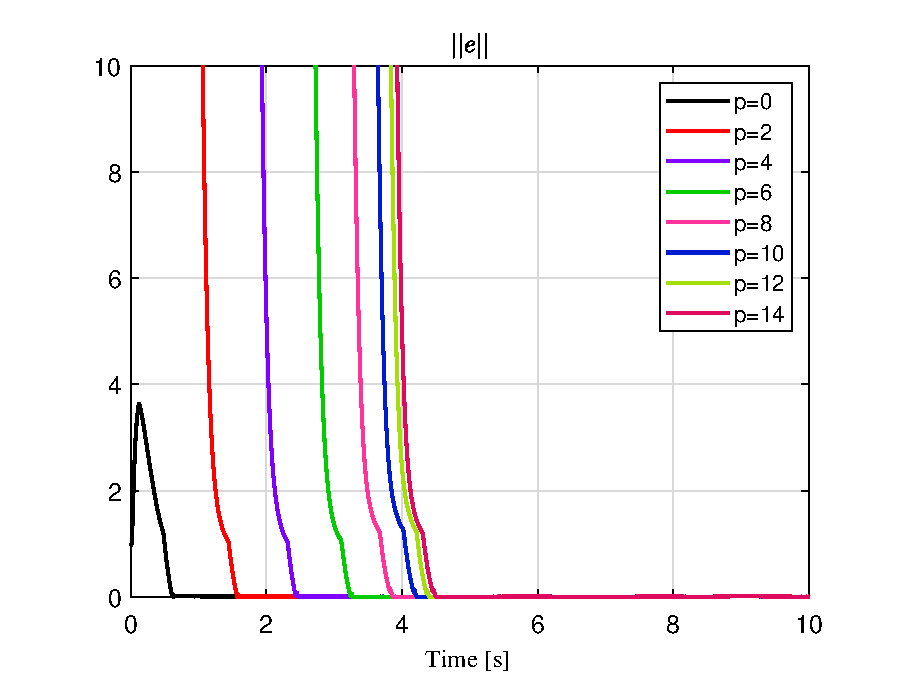
\includegraphics[width=9cm]{sys_4s_disc_FxT_error_orders.eps}}
% 		\caption[SISO HOSM-UIO Fixed-Time estimation]{HOSM-UIO. Estimation error with different orders at initial error $e_0$ showing fixed-time estimation. With $\hat{x}_{0,j}=1\times 10^{p},j=1,...,4$.
% 		}
% 	\label{fig: CH4 Error 4s norm with orders}
% \end{figure}

% \begin{figure}[htbp]
% 	\centering{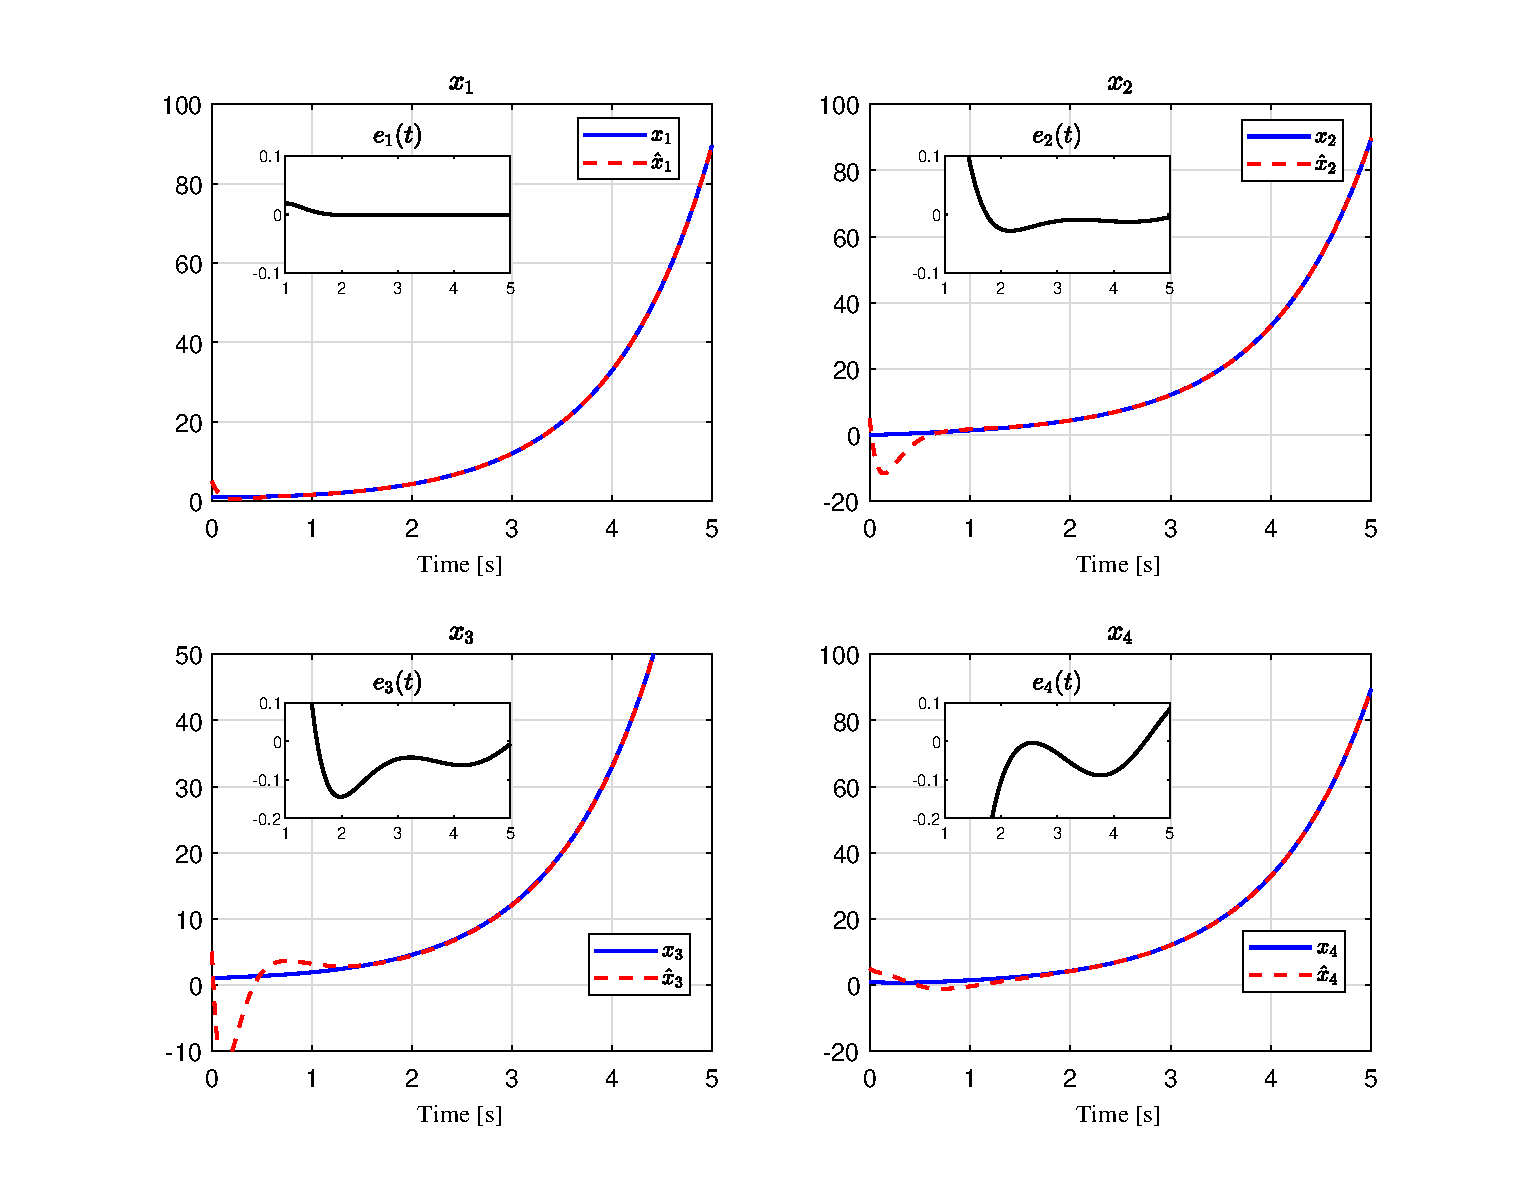
\includegraphics[width=15.8cm]{sys_4s_linear_states.eps}}
% 	\caption[SISO Linear UIO]{Linear UIO. Plant state $x$, state estimation $\hat{x}$ and estimation errors $e=\hat{x}-x$.}
% 	\label{fig: CH4 Error 4s states and norm, e_0 linear}
% \end{figure}

% \begin{figure}[htbp]
% 	\centering{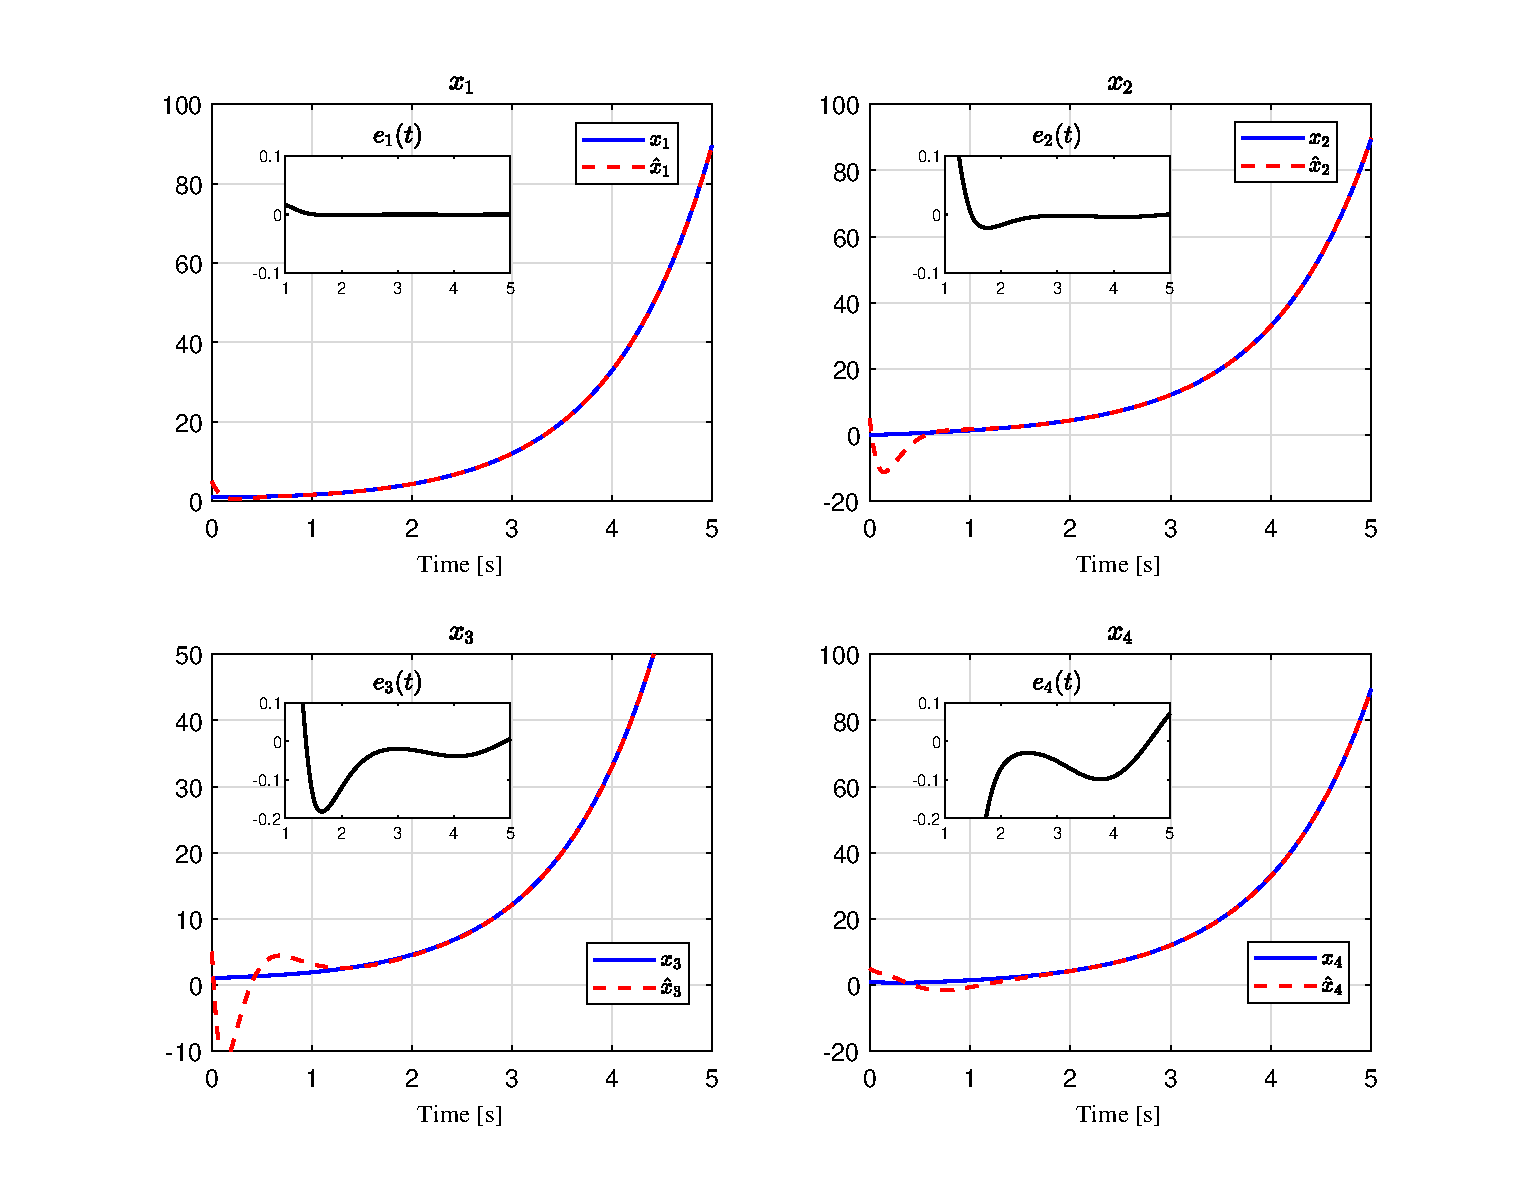
\includegraphics[width=17cm]{sys_4s_cont_states.eps}}
% 	\caption[SISO Continuous UIO]{Continuous UIO. Plant state $x$, state estimation $\hat{x}$ and estimation errors $e=\hat{x}-x$.}
% 	\label{fig: CH4 Error 4s states and norm, e_0 cont}
% \end{figure}

% \begin{figure}[htbp]
% 	\centering{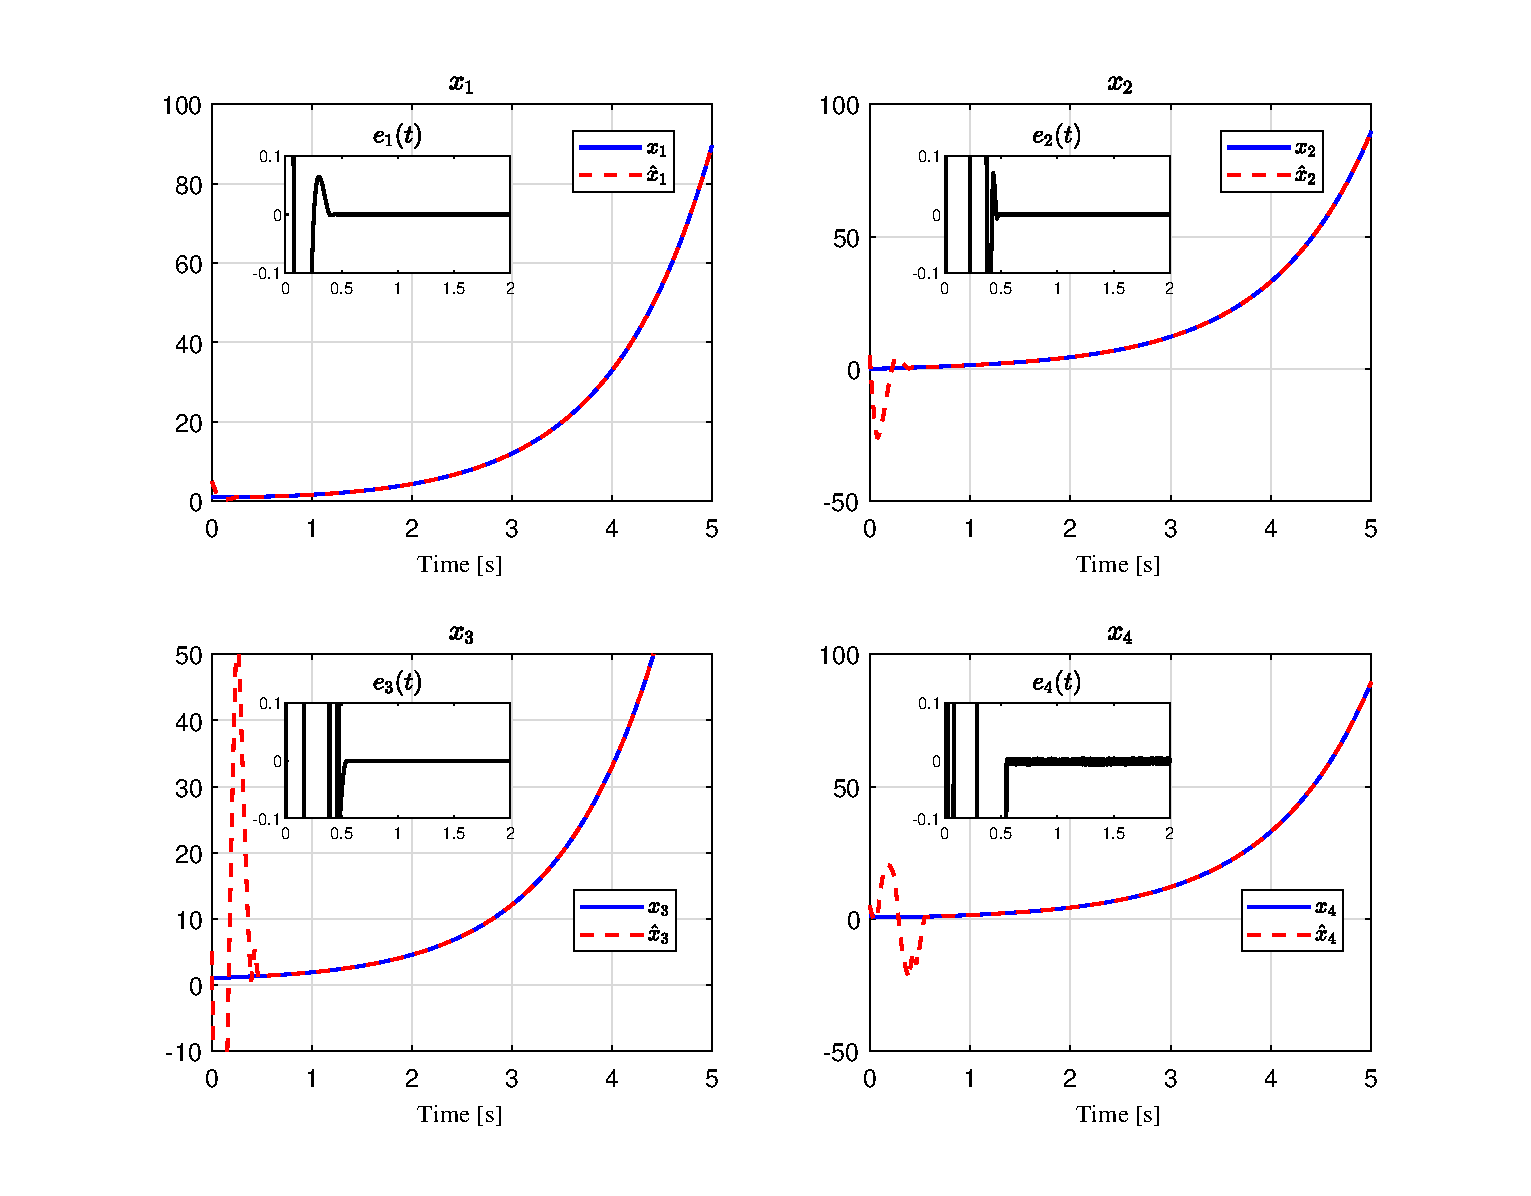
\includegraphics[width=17cm]{sys_4s_disc_states.eps}}
% 	\caption[SISO HOSM-UIO]{HOSM-UIO. Plant state $x$, state estimation $\hat{x}$ and estimation errors $e=\hat{x}-x$.}
% 	\label{fig: CH4 Error 4s states and norm, e_0 disc}
% \end{figure}




\chapter{Calculo de ganancias para CTA} \label{Cap4}
\section{Para grado relativo 3}
\section{Implementacion en Matalab}
%\section{Para grado relativo 4}
%\section{Para grado relativo 5}


%%%%%%%%%%%%%%%%%%%%%%%%%%%%%%%%%%%%%%%%%%%%%%%%%%%%%%%%%%%%%
%%
%%			Ejemplo empieza
%%
%%%%%%%%%%%%%%%%%%%%%%%%%%%%%%%%%%%%%%%%%%%%%%%%%%%%%%%%%%%%%%%
% In this chapter we present the second part of the main result in this work. We introduce the design of Bl-homogeneous Unknown Input Observers (UIO) for MIMO-LTI systems assuming strong observability. The idea is to transform the system in to a Special Coordinate Basis, (detailed in Chapter 2) obtaining a  convenient representation of the system for the observer design, but more general than the used in previous works, for example the MIMO observer form used in \cite{Niederwieser2021} which decompose the system in a set of subsystems conveniently interconnected in a 'triangular' form (see Section \ref{sec: CH1 Literature}, Equation \eqref{ecu: Niederwieser SCB}). Even though such an observer form of the system is a great feature obtained for linear systems and greatly simplifies convergence analysis, it is shown that the observers designed here can deal with a more general type of interconnections between subsystems.

% Here we use directly a discontinuous nonlinear observer instead of differentiators. This fact suppress the necessity of using a cascade scheme composed by a linear observer and a discontinuous differentiator.

% As in the SISO case, the nonlinear injection terms will be designed to accelerate the convergence as much as we want by selecting appropriate and sufficiently large gains. Even more, due to the assignability of bl-homogeneous degrees in the observer, we can reach and assure exactly and finite-time (or moreover fixed-time) estimation of the states in presence of unknown inputs.
	
% \section{Unknown input observers for LTI-MIMO systems}
% Consider the MIMO-LTI system without feedthrough (for simplicity) given by
% \begin{equation}
% 	\begin{split}\label{ecu: CH4 Sys MIMO orig}
% 	\Sigma: \left\{
% 	\begin{array}{rl}
% 		\dot{x} &= Ax + D\omega\\
% 		y&=Cx
% 	\end{array}
% 	\right. \\
% 	\end{split}
% \end{equation}
% where $x \in \RE^n$ is the state vector, $\omega \in \RE^m$ the unknown input vector and $y \in \RE^p$ is the output vector. Accordingly, the matrices $A,D,C$ have appropriate dimensions. For simplicity in the development we do not consider known inputs $u$, since it does not modify the (observability) properties and it is simple to include it in the observer design. 

% The task is to build an unknown input observer (UIO) providing for finite-time (preferably fixed-time) estimation of the states in presence of the unknown inputs. In chapter 2 we have stated the necessary and sufficient conditions for the existence and of UIO with arbitrary unknown inputs. We assume to have strong observability only. In Chapter 3 we have introduced this observers in the SISO case. This Chapter generalize the results to arbitrary number of inputs and outputs.

% The equations in the observer are understood in the Filippov sense \cite{Filippov1988} in order to provide for the possibility to use discontinuous signals. Note that Filippov solutions coincide with the usual solutions, when the right-hand sides are continuous.

% Special Coordinate Basis (SCB) is a useful tool to represent a system in an appropriate form for the observer design.

% %Another characterization for strongly observable LTI systems in terms of the relative degree with respect to the unknown input was introduced in \cite{Fridman2006}.
% %
% %\begin{definition}
% %	Following \cite{Isidori1996} the relative degree of system \eqref{ecu: Sys siso orig} with respect to the unknown input is the number $r$ such that
% %	\begin{equation}
% %		CA^jD=0. \quad j=1,...,r-2, \quad CA^{r-1}D \neq 0
% %	\end{equation}
% %\end{definition}
% %Since the system \eqref{ecu: Sys siso orig} is assumed to be observable (in absence of unknown input), i.e. the matrix 
% %
% %\begin{equation}
% %	\mathcal{O} = \begin{bmatrix}
% %		C \\
% %		CA \\
% %		\vdots \\
% %		CA^{n-1}
% %	\end{bmatrix}
% %\end{equation}
% %
% %has full rank. Then we can transform the system to the observability canonical form through the state transformation $T=\mathcal{O}^{-1}$, such that the matrices $A,D,C$ take the form

% \subsection{Unknown Input Observer design}
% Given a strongly observable system $\Sigma$ in \eqref{ecu: CH4 Sys MIMO orig} under SCB transformation detailed in Section \ref{sec: CH2 SCB} a transformed system is obtained, if we take into account the Property \ref{prop: CH2 SCB strong obsv} this transformed system $\Sigma_{SCB}(\Sigma_b,\Sigma_d)$ is described by the following set.

% Subsystems $\Sigma_{b,\iota}$ with associated states $x_{b,\iota}\in \RE^{n_{b,\iota}}, \iota=1,...,p_b$ 
% \begin{equation}
% 	\begin{split}\label{ecu: CH4 Sigma_b}
% 		\Sigma_{b,\iota}: \left\{
% 		\begin{array}{rl}
% 		\dot{x}_{b,\iota,1} &= x_{b,\iota,2} + H_{bd,\iota,1}y_d, \quad y_{b,\iota}=x_{b,\iota,1}, \\
% 		\dot{x}_{b,\iota,j} &= x_{b,\iota,j+1} + H_{bd,\iota,j}y_d, \\
% 		& \vdots \quad j=2,...,n_{b,\iota}-1\\
% 		\dot{x}_{b,\iota,n_{b,\iota}} &= A_{bb,\iota}x_{b} + H_{bd,\iota,n_{b,\iota}}y_d, 
% 	\end{array}
% \right. \\
% 	\end{split}
% \end{equation}
% with $\sum_{\iota=1}^{p_b}n_{b,\iota}=n_b$.

% and subsystems $\Sigma_{d,i}$ with associated states $x_{d,i} \in \RE^{n_{d,i}}, i=1,...,p_d$ 
% \begin{equation}
% 	\begin{split}\label{ecu: CH4 Sigma_d}
% 		\Sigma_{d,i}: \left\{
% 		\begin{array}{rl}
% 		\dot{x}_{d,i,1} &= x_{d,i,2} + H_{dd,i,1}y_d,  \quad y_{d,i} = x_{d,i,1} \\
% 		\dot{x}_{d,i,j} &= x_{c,i,j+1} + H_{dd,i,j}y_d, \\
% 		& \vdots \quad j=2,...,n_{d,i}-1\\
% 		\dot{x}_{d,i,n_{d,i}} &= A_{db,i}x_b + A_{dd,i}x_d + w_{d,i},
% 	\end{array}
% \right. \\ 
% 	\end{split}
% \end{equation}
% similarly $\sum_{i=1}^{p_d}n_{d,i}=n_d$. And therefore $n_b+n_d=n$.

% Where $A_{bb,\iota},H_{bd,\iota,j},A_{dd,i},A_{db,i},H_{dd,i,j}$ are constant row vectors of appropriate dimensions. Recall that $\Sigma_b$ corresponds to the observable dynamics of the system, and $\Sigma_d$ corresponds to the strongly observable dynamics. It is clear that the subsystems can be expressed in observer or observability form, as we say before, the first option allows us to apply directly an homogeneous differentiator as an state observer \cite{Niederwieser2021}, but it can not be applied in the observability form. The observability form requires the bl-homogeneity of the observer. This fact have been shown in SISO case at previous Chapter.

% \begin{assumtion}\label{Assum: CH4 omega}
% 	Unknown input $\omega(t)$ is a uniformly bounded function $\norm{\omega(t)}\leq \Delta$, equivalently, each element of the vector $|w_{d,i}(t)|\leq \Delta_{i} \in \mathbb{R}_{\geq 0}, i=1,...,p_d$.
% \end{assumtion}
% This allow us to relax the existence conditions of UIO in other to have an observer under strong observability only, see Section \ref{sec: CH2 Cond existence}. The relative degree of the outputs $y_{d,i}$ with respect to the unknown input is $n_{d,i}$.

% The observer $\Omega(\Omega_b,\Omega_d)$ is given by
% \begin{equation}
% 	\begin{split}\label{ecu: CH4 Omega_b}
% 		\Omega_{b,\iota}: \left\{
% 		\begin{array}{rl}
% 			\dot{\hat{x}}_{b,\iota,1} &= -k_{b,\iota,1}L \tilde{\phi}_{b,\iota,1}( \hat{x}_{b,\iota,1}-y_{b,\iota} ) + \hat{x}_{b,\iota,2} + H_{bd,\iota,1}y_d \\
% 			\dot{\hat{x}}_{b,\iota,j} &= -k_{b,\iota,j}L^{j} \tilde{\phi}_{b,\iota,j}( \hat{x}_{b,\iota,1}-y_{b,\iota} ) + \hat{x}_{b,\iota,j+1} + H_{bd,\iota,j}y_d  \\
% 			\vdots \quad & j=2,...,n_{b,\iota}-1\\
% 			\dot{\hat{x}}_{b,\iota,n_{b,\iota}} &= -k_{b,\iota,n_{b,\iota}}L^{n_{b,\iota}} \tilde{\phi}_{b,\iota,n_{b,\iota}}( \hat{x}_{b,\iota,1}-y_{b,\iota} ) + A_{bb,\iota}\hat{x}_{b}  + H_{bd,\iota,n_{b,\iota}}y_d 
% 		\end{array}
% 		\right. \\
% 	\end{split}
% \end{equation}
% \begin{equation}
% 	\begin{split}\label{ecu: CH4 Omega_d}
% 		\Omega_{d,i}: \left\{
% 		\begin{array}{rl}
% 			\dot{\hat{x}}_{d,i,1} &= -k_{d,i,1}L \tilde{\phi}_{d,i,1}( \hat{x}_{d,i,1}-y_{d,i} ) + \hat{x}_{d,i,2} + H_{dd,i,1}y_d,  \\
% 			\dot{\hat{x}}_{d,i,j} &= -k_{d,i,j}L^{j}\tilde{\phi}_{d,i,j}( \hat{x}_{d,i,1}-y_{d,i} ) + \hat{x}_{d,i,j+1} + H_{dd,i,j}y_d,\\
% 			\vdots \quad & j=2,...,n_{d,i}-1\\
% 			\dot{\hat{x}}_{d,i,q_i} &= -k_{d,i,q_i}L^{n_{d,i}} \tilde{\phi}_{d,i,q_i}( \hat{x}_{d,i,1}-y_{d,i} ) + A_{db,i}\hat{x}_b + A_{dd,i}\hat{x}_d
% 		\end{array}
% 		\right. \\
% 	\end{split}
% \end{equation}
% with positive external gains $k_{b,\iota,j}>0,k_{d,i,j}>0$ and positive tuning gains $\alpha>0,L >0$, appropriately selected as it will be show latter. 

% In $\Omega_b$ the nonlinear output injection terms $\tilde{\phi}_{b,\iota,j}(\cdot)$ are obtained from the functions

% \begin{equation}\label{ecu: CH4 Injection Sigma_b}
% 	\phi_{b,\iota,j}(s) = \kappa_{b,\iota j} \sig{s}{\frac{r_{(b,\iota),0,j+1}}{r_{(b,\iota),0,1}}} + \theta_{b,\iota j} \sig{s}{\frac{r_{(b,\iota),\infty,j+1}}{r_{(b,\iota),\infty,1}}}
% \end{equation}
% by scaling the positive internal gains $\kappa_{b,\iota j}>0,\theta_{b,\iota j}>0$
% \begin{equation}
% 	\kappa_{b,\iota j} \rightarrow \left( \frac{L^{n_{b,\iota}}}{\alpha}\right)^{\frac{jd_0}{r_{(b,\iota),0,1}}}\kappa_{b,\iota j} ,\qquad \theta_{b,\iota j} \rightarrow \left( \frac{L^{n_{b,\iota}}}{\alpha}\right)^{\frac{jd_{\infty}}{r_{(b,\iota),\infty,1}}}\theta_{b,\iota j}
% \end{equation}
% with powers selected as $r_{(b,\iota),0,n_{b,\iota}}=r_{(b,\iota),\infty,n_{b,\iota}}=1$, and
% \begin{equation}\label{ecu: r-siso}
% 	\begin{split}
% 		r_{(b,\iota),j,n_{b,\iota}} = r_{(b,\iota),0,j+1}-d_0 = 1-(n_{b,\iota}-j)d_0 \\
% 		r_{(b,\iota),j,n_{b,\iota}} = r_{(b,\iota),\infty,j+1}-d_{\infty} = 1-(n_{b,\iota}-j)d_{\infty}
% 	\end{split}
% \end{equation}
% which are completely defined by two parameters $d_0,d_{\infty}$.

% Similarly, for $\Omega_d$, the nonlinear output injection terms $\tilde{\phi}_{d,i,j}$ are obtained from the functions 
% \begin{equation}\label{ecu: CH4 Injection Sigma_d}
% 	\phi_{d,i,j}(s) = \kappa_{d,i j} \lceil s \rfloor^{\frac{r_{(d,i),0,j+1}}{r_{(d,i),0,1}}} + \theta_{d,i j} \lceil s \rfloor^{\frac{r_{(d,i),\infty,j+1}}{r_{(d,i),\infty,1}}}
% \end{equation}

% by scaling the positive internal gains $\kappa_{d,i j}>0,\theta_{d,i j}>0$
% \begin{equation}
% 	\kappa_{d,i j} \rightarrow \left( \frac{L^{n_{d,i}}}{\alpha}\right)^{\frac{jd_0}{r_{(d,i),0,1}}}\kappa_{d,i j} ,\qquad \theta_{d,i j} \rightarrow \left( \frac{L^{n_{d,i}}}{\alpha}\right)^{\frac{jd_{\infty}}{r_{(d,i),\infty,1}}}\theta_{d,i j}
% \end{equation}

% with powers selected as $r_{(d,i ),0,n_{d,i}}=r_{(d,i),\infty,n_{d,i}}=1$, and
% \begin{equation}
% 	\begin{split}
% 		r_{(d,i),j,n_{d,i}} = r_{(d,i),0,j+1}-d_0 = 1-(n_{d,i}-j)d_0 \\
% 		r_{(d,i),j,n_{d,i}} = r_{(d,i),\infty,j+1}-d_{\infty} = 1-(n_{d,i}-j)d_{\infty}
% 	\end{split}
% \end{equation}

% which are completely defined by the same parameters $d_0,d_{\infty}$. They have to satisfy
% \begin{equation}\label{ecu: CH4 d0dinf}
% 	-1\leq d_0 \leq d_{\infty} < \min_{\begin{array}{ll}
% 			\iota=1,...,p_b, \\
% 			i=1,...,p_d
% 	\end{array} } 
% 	\left\{ \frac{1}{n_{b,\iota}-1},\frac{1}{n_{d,i}-1}  \right\}
% \end{equation}

% We have to highlight the fact that nonlinear injection terms in \eqref{ecu: CH4 Injection Sigma_b} and \eqref{ecu: CH4 Injection Sigma_d} are very similar to them in the bl-homogeneous differentiator \cite{Moreno2021} but the terms given here are simpler. This simplifies the task of implementation.

% \subsection{Gain Selection}
% 	Each type of gains in the observer has a different role, and the idea in the gain tuning is very intuitive. For simplicity in explanation we take hereafter $\psi=\{(b,\iota),(d,i)\}$ to refer to both types of subsystems.
% 	\begin{enumerate}
% 		\item The internal gains $\kappa_{\psi,j} > 0, \theta_{\psi,j} > 0$ can be selected arbitrary. These positive real values correspond to the desired weighting of each term of low degree and high degree respectively of $\phi_{\psi,j}$.
% 		\item The external gains $k_{\psi,j} > 0$ have the objective of stabilizing the observer in absence of interconnections and external perturbations, i.e. when $A_{bb}=A_{db}=A_{dd}=0$ and $\omega(t)=0$.
% 		\item Parameter $L$ is selected large enough to assure the convergence in presence of interconnections, but not of the bounded perturbations $\omega(t)$. Setting its value grater than minimal value to assure stability the convergence velocity will be increased.
% 		\item The tuning parameter $\alpha$ is selected large enough to assure the convergence in presence of the unknown bounded inputs $\omega(t)$.
% 	\end{enumerate}

% \subsection{Estimation in original coordinates}
% The estimated state obtained from the observer $\Omega(\Omega_b,\Omega_d)$ in \eqref{ecu: CH4 Omega_b},\eqref{ecu: CH4 Omega_d} corresponds to the transformed system $\Sigma_{SCB}$ in \eqref{ecu: CH4 Sigma_b},\eqref{ecu: CH4 Sigma_d} represented in SCB coordinates through the state $\Gamma_s$, input $\Gamma_i$ and output $\Gamma_o$ transformations \eqref{ecu: CH2 SCB transformation}, moreover it was applied an extra transformation $\Gamma_{\mathcal{O}}$ given by $\Gamma_{\mathcal{O}}=\text{diag}\left\lbrace\mathcal{O}_{b,1}^{-1},...,\mathcal{O}_{b,p_b}^{-1},\mathcal{O}_{d,1}^{-1},...,\mathcal{O}_{d,p_d}^{-1} \right\rbrace$ which puts the subsystems in observability canonical form.

% The states in original coordinates can be computed as
% \begin{equation}\label{ecu: CH4 invers transf}
% 	x = \Gamma_s\Gamma_{\mathcal{O}}\hat{x}
% \end{equation}

% Therefore, the observer in original coordinates for the system \eqref{ecu: CH4 Sys MIMO orig} takes the form
% %
% %\begin{equation}
% %	x = \Gamma_s\Gamma_{\mathcal{O}}\hat{x}
% %\end{equation}
% \begin{equation}\label{ecu: CH4 Observer Orig Coord}
% 	\begin{split}
% 		\dot{\hat{x}} &= -\Gamma_s\Gamma_{\mathcal{O}} K\Phi(e_y) + A\hat{x} + Bu \\
% 		e_y &= \Gamma_o^{-1}(\hat{y}-y)\\
% 		\hat{y} &= C\hat{x}
% 	\end{split}
% \end{equation}
% with
% \begin{equation}\label{ecu: CH4 Observer Orig Coord K}
% 	\begin{split}
% 		K &= \text{diag}(K_{b,1},...,K_{b,p_b},K_{d,1},...,K_{d,p_d})\\
% 		K_{b,\iota}&=\begin{bmatrix}
% 			k_{\iota}L & & & \\
% 			& k_{b,\iota}L^2 & & \\
% 			&        & \ddots & \\
% 			&        &        & k_{b,\iota}L^{n_{\iota}}
% 		\end{bmatrix}, \quad \iota=1,...,p_b\\
% 		K_{d,i}&=\begin{bmatrix}
% 			k_{i}L & & & \\
% 			& k_{d,i}L^2 & & \\
% 			&        & \ddots & \\
% 			&        &        & k_{d,i}L^{n_{i}}
% 		\end{bmatrix}, \quad i=1,...,p_d
% 	\end{split}
% \end{equation}
% \begin{equation}\label{ecu: CH4 Observer Orig Phi}
% 	\begin{split}
% 		\Phi(e_y) =
% 		\Bigl[	\Phi_{b,1}( e_y ) \quad \Phi_{b,2}( e_y ) \quad ,\hdots, \quad \Phi_{b,n_b}( e_y ),\Bigr. \\
% 		\Bigl.\Phi_{d,1}( e_y ) \quad \Phi_{d,2}( e_y ) \quad ,\hdots, \quad \Phi_{d,n_d}( e_y )\Bigr]^T \\
% 	\end{split}
% \end{equation}
% \begin{equation}\label{ecu: CH4 Observer Orig phi}
% 	\begin{split}
% 		&\Phi_{b,\iota}(e_y) =
% 		\begin{bmatrix}
% 			\tilde{\phi}_{b,\iota,1}( e_y ) & \tilde{\phi}_{b,\iota,2}( e_y ) & ,\hdots, & \tilde{\phi}_{b,\iota,n_b}( e_y )
% 		\end{bmatrix}^T, \quad \iota = 1,...,p_b \\
% 		&\Phi_{d,i}(e_y) =
% 		\begin{bmatrix}
% 			\tilde{\phi}_{d,i,1}( e_y ) & \tilde{\phi}_{d,i,2}( e_y ) & ,\hdots, & \tilde{\phi}_{d,i,n_d}( e_y )
% 		\end{bmatrix}^T, \quad i = 1,...,p_d
% 	\end{split}
% \end{equation}


% \subsection{Main result. UIO - MIMO case}
% The main result of this work in the MIMO case establishes that the bl-homogeneous Unknown Input Observer \eqref{ecu: CH4 Observer Orig Coord}, is able to estimate at least asymptotically the states of a strongly observable linear system \eqref{ecu: CH4 Sys MIMO orig}.

% \begin{theorem}\label{theo: CH4 Obsv MIMO}
% 	Let the strongly observable MIMO-LTI system $\Sigma$ \eqref{ecu: CH4 Sys MIMO orig} in original coordinates has an UIO given by \eqref{ecu: CH4 Observer Orig Coord}-\eqref{ecu: CH4 Observer Orig phi}. Selecting $d_0,d_{\infty}$ as in \eqref{ecu: CH4 d0dinf} and choosing arbitrary (internal gains)  $\kappa_{\psi,j}>0$ and $\theta_{\psi,j}>0$, with $\psi=\{(b,\iota),(d,i)\}$. Suppose that either $\Delta_i=0,i=1,...,p_d$ or $d_0=-1$. Under this conditions,  there exist appropriate gains $k_{\psi,j}>0$ with $\psi=\{(b,\iota),(d,i)\}$, and parameters $L>0,\alpha>0$ sufficiently large such that the solutions of bl-homogeneous UIO converge globally and asymptotically to the true states of $\Sigma$, i.e. $\hat{x}_j(t) \rightarrow x_j(t)$ as $t \rightarrow \infty$. 
	
% 	In particular, we have we have the following convergence properties and assignment.
% 	\begin{itemize}
% 		\item The observer $\Omega_{b,\iota}$ in \eqref{ecu: CH4 Omega_b} has assignable dynamics and they can converge globally and 
% 		\begin{enumerate}
% 			\item Exponentially if $d_0=0$
% 			\item Finite-time if $d_0 < 0$
% 			\item Fixed-time if $d_0 < 0 < d_\infty$
% 		\end{enumerate}
% 			\item The observer $\Omega_{d,i}$ in \eqref{ecu: CH4 Omega_d} has assignable dynamics and they can converge globally and 
% 			\begin{enumerate}
% 				\item Exponentially if
% 				\begin{equation}
% 					d_0=0 \quad\text{with}\quad \Delta_i \equiv 0,
% 				\end{equation}
% 				\item Finite-time if 
% 				\begin{equation}
% 					\begin{split}
% 						&(a) \quad -1 < d_0 < 0, \quad \Delta_i \equiv 0, \quad or  \\
% 						&(b) \quad d_0 =-1, \quad  \Delta_i\neq 0
% 					\end{split}
% 				\end{equation}
% 				\item Fixed-time if
% 				\begin{equation}
% 					\begin{split}
% 						&(a) \quad -1 < d_0 < 0 < d_\infty,\quad \Delta_i \equiv 0,  \quad or \\
% 						&(b) \quad -1 = d_0 < 0 < d_\infty,\quad \Delta_i \neq 0.
% 					\end{split}
% 				\end{equation} 
% 			with $d_{\infty}$ always subject to \eqref{ecu: CH4 d0dinf} be fullfiled.
% 			\end{enumerate}
% 	\end{itemize}
% \end{theorem}

% \newpage
% \subsection[Proof]{Proof of Theorem \ref{theo: CH4 Obsv MIMO}}
% The proof, similar to the SISO case will be carried out in a Lyapunov framework through a bl-homogeneous Lyapunov function (Bl-LF), composed of a sum of Bl-LFs related to each subsystem.

% To study the error system in a more suitable form, we are going to take the system and observer in the transformed SCB coordinates, i.e. the system \eqref{ecu: CH4 Sigma_b},\eqref{ecu: CH4 Sigma_d} and observer \eqref{ecu: CH4 Omega_b},\eqref{ecu: CH4 Omega_d}. It is clear that the analysis is completely equivalent in original coordinates.
	
% Let the estimation error variables 
% \begin{equation}
% 	\begin{split}\label{error variables}
% 		e_{b,\iota,j}=\hat{x}_{b,\iota,j}-x_{b,\iota,j}, \quad \iota=1,...,p_b, j=1,...,n_{b,\iota}, \\
% 		e_{d,i,j}=\hat{x}_{d,i,j}-x_{d,i,j}, \quad i=1,...,p_b, j=1,...,n_{d,i},
% 	\end{split}
% \end{equation}
% The dynamics error are described by

% \begin{equation}
% 	\begin{split}\label{eb1}
% 		\Xi_{b,\iota}: \left\{
% 		\begin{array}{rl}
% 			\dot{e}_{b,\iota,1} &= -k_{b,\iota,1}L \tilde{\phi}_{b,\iota,1}( e_{b,\iota,1} ) + e_{b,\iota,2} \\
% 			\dot{e}_{b,\iota,j} &= -k_{b,\iota,j}L^{j} \tilde{\phi}_{b,\iota,j}( e_{b,\iota,1} ) + e_{b,\iota,j+1} \\
% 			\vdots \quad & j=2,...,n_{b,\iota}-1\\
% 			\dot{e}_{b,\iota,n_{b,\iota}} &= -k_{b,\iota,n_{b,\iota}}L^{n_{b,\iota}} \tilde{\phi}_{b,\iota,n_{b,\iota}}( e_{b,\iota,1} ) + A_{bb,\iota}e_{b}
% 		\end{array}
% 		\right. \\
% 	\end{split}
% \end{equation}

% \begin{equation}
% 	\begin{split}\label{ed1}
% 		\Xi_{d,i}: \left\{
% 		\begin{array}{rl}
% 			\dot{e}_{d,i,1} &= -k_{d,i,1}L \tilde{\phi}_{d,i,1}( e_{d,i,1} ) + e_{d,i,2} \\
% 			\dot{e}_{d,i,j} &= -k_{d,i,j}L^{j}\tilde{\phi}_{d,i,j}( e_{d,i,1} ) + e_{d,i,j+1} \\
% 			\vdots \quad & j=2,...,n_{d,i}-1\\
% 			\dot{e}_{d,i,q_i} &= -k_{d,i,q_i}L^{n_{d,i}} \tilde{\phi}_{d,i,q_i}( e_{d,i,1} ) + A_{db,i}e_b + A_{dd,i}e_d - \omega_{d,i}
% 		\end{array}
% 		\right. \\
% 	\end{split}
% \end{equation}
% for $\iota=1,2,...,p_b, i=1,2,...,p_d$.

% Applying the time scaling via the next transformation	
% \begin{equation}
% 	\epsilon_{b,\iota,j}=\frac{L^{n_{b,\iota}-j+1}}{\alpha}e_{b,\iota,j},\qquad \epsilon_{d,i,j}=\frac{L^{n_{d,i}-j+1}}{\alpha}e_{d,i,j}
% \end{equation}
% 	we obtain 
% \begin{equation}
% 	\begin{split}\label{ecu: CH4 Error1b}
% 		\Xi_{b,\iota}: \left\{
% 		\begin{array}{rl}
% 			\dot{\epsilon}_{b,\iota,1} &= L\left[ -k_{b,\iota,1}\phi_{b,\iota,1}( \epsilon_{b,\iota,1} ) + \epsilon_{b,\iota,2} \right] \\
% 			\dot{\epsilon}_{b,\iota,j} &= L\left[ -k_{b,\iota,j} \phi_{b,\iota,j}( \epsilon_{b,\iota,1} ) + \epsilon_{b,\iota,j+1} \right] \\
% 			\vdots \quad & j=2,...,n_{b,\iota}-1\\
% 			\dot{\epsilon}_{b,\iota,n_{b,\iota}} &= L\left[ -k_{b,\iota,n_{b,\iota}} \phi_{b,\iota,n_{b,\iota}}( \epsilon_{b,\iota,1} ) + \frac{1}{\alpha}\mu_{\iota}(\epsilon_b) \right]
% 		\end{array}
% 		\right. \\
% 	\end{split}
% \end{equation}

% \begin{equation}
% 	\begin{split}\label{ecu: CH4 Error1d}
% 		\Xi_{d,i}: \left\{
% 		\begin{array}{rl}
% 			\dot{\epsilon}_{d,i,1} &= L\left[ -k_{d,i,1} \phi_{d,i,1}( \epsilon_{d,i,1} ) + \epsilon_{d,i,2} \right] \\
% 			\dot{\epsilon}_{d,i,j} &= L\left[ -k_{d,i,j} \phi_{d,i,j}( \epsilon_{d,i,1} ) + \epsilon_{d,i,j+1} \right] \\
% 			\vdots \quad & j=2,...,n_{d,i}-1\\
% 			\dot{\epsilon}_{d,i,q_i} &= L\left[ -k_{d,i,q_i} \phi_{d,i,q_i}( \epsilon_{d,i,1} ) + \frac{1}{\alpha}\Psi_{i}(\epsilon_b,\epsilon_d,\omega_{d,i}) \right]
% 		\end{array}
% 		\right. \\
% 	\end{split}
% \end{equation}
% 	where
% \begin{equation}
% 	\begin{split}
% 		\mu_{\iota}(\epsilon_b) &= A_{bb,\iota}e_b = \sum_{j=1}^{p_b}\sum_{k=1}^{n_{b,j}} a_{(bb,\iota),j,k} e_{b,j,k}= \alpha\sum_{j=1}^{p_b}\sum_{k=1}^{n_{b,j}} \frac{a_{(bb,\iota),j,k}}{L^{n_{b,\iota}-k+1}}\epsilon_{b,j,k} \\
% 		\Psi_{i}(\epsilon_b,\epsilon_d,\omega_{d,i}) &= A_{db,i}e_b + A_{dd,i}e_d - \omega_{d,i} \\
% 		&=\sum_{j=1}^{p_b}\sum_{k=1}^{n_{b,j}} a_{(db,i),j,k}e_{b,j,k} + \sum_{j=1}^{p_d}\sum_{k=1}^{n_{d,j}} a_{(dd,i),j,k}e_{d,j,k} - \omega_{d,i} \\
% 		&=\alpha \sum_{j=1}^{p_b}\sum_{k=1}^{n_{b,j}}  \frac{a_{(db,i),j,k}}{L^{n_{b,j}-k+1}} \epsilon_{b,j,k}
% 		+ \alpha \sum_{j=1}^{p_d}\sum_{k=1}^{n_{d,j}}  \frac{a_{(dd,i),j,k}}{L^{n_{d,j}-k+1}} \epsilon_{d,j,k}
% 	\end{split} 
% \end{equation}
% 	the fact that $\tilde{\phi}_{\psi,j}( \frac{\alpha}{L^n}s ) = \frac{\alpha}{L^n}\tilde{\phi}_{\psi,j}(s)$ has been used.
	
% 	For the convergence proof, it is convenient to perform another state transformation
% \begin{equation}
% 	\begin{split}
% 		z_{b,\iota,j} = \frac{\epsilon_{b,i,j}}{k_{b,\iota,j-1}},\quad \iota=1,...,p_b, j=1,...,n_{b,\iota} \\
% 		z_{d,i,j} = \frac{\epsilon_{d,i,j}}{k_{d,i,j-1}},\quad i=1,...,p_d, j=1,...,n_{d,i}
% 	\end{split}
% \end{equation}
% 	Then \eqref{ecu: CH4 Error1b} and \eqref{ecu: CH4 Error1d} become
% \begin{equation}
% 	\begin{split}\label{ecu: CH4 Error2b}
% 		\Xi^*_{b,\iota}: \left\{
% 		\begin{array}{rl}
% 			z'_{b,\iota,1} &= -\tilde{k}_{b,\iota,1}\left( \phi_{b,\iota,1}( z_{b,\iota,1} ) + z_{b,\iota,2} \right) \\
% 			z'_{b,\iota,j} &= -\tilde{k}_{b,\iota,j}\left( \phi_{b,\iota,j}( z_{b,\iota,1} ) + z_{b,\iota,j+1} \right)  \\
% 			\vdots \quad & j=2,...,n_{b,\iota}-1\\
% 			z'_{b,\iota,n_{b,\iota}} &= -\tilde{k}_{b,\iota,n_{b,\iota}} \phi_{b,\iota,n_{b,\iota}}( z_{b,\iota,1} ) + \tilde{\mu}_{\iota}(z_b)
% 		\end{array}
% 		\right. \\
% 	\end{split}
% \end{equation}

% \begin{equation}
% 	\begin{split}\label{ecu: CH4 Error2d}
% 		\Xi^*_{d,i}: \left\{
% 		\begin{array}{rl}
% 			z'_{d,i,1} &= -\tilde{k}_{d,i,1}\left( \phi_{d,i,1}( z_{d,i,1} ) + z_{d,i,2} \right)  \\
% 			z'_{d,i,j} &= -\tilde{k}_{d,i,j}\left( \phi_{d,i,j}( z_{d,i,1} ) + z_{d,i,j+1} \right)  \\
% 			\vdots \quad & j=2,...,n_{d,i}-1\\
% 			z'_{d,i,q_i} &= -\tilde{k}_{d,i,q_i} \phi_{d,i,q_i}( z_{d,i,1} ) + \tilde{\Psi}_{i}(z_b,z_d,\omega_{d,i})
% 		\end{array}
% 		\right. \\
% 	\end{split}
% \end{equation}
% with $\tilde{k}_{b,\iota,j}=\frac{k_{b,\iota,j}}{k_{b,\iota,j-1}}$, $\tilde{k}_{d,i,j}=\frac{k_{d,i,j}}{k_{d,i,j-1}}, \quad k_{b,\iota,0} = k_{d,i,0} = 1$

% where
% \begin{equation}
% 	\begin{split}\label{ecu: CH4 mu_tilde}
% 		\tilde{\mu}_{\iota}(z_b) &= \frac{1}{k_{b,\iota,n_{b,\iota-1}}}\sum_{j=1}^{p_b}\sum_{k=1}^{n_{b,j}} \frac{a_{(bb,\iota),j,k}k_{b,j,k-1}}{L^{n_{b,j}-k+1}}z_{b,j,k} 
% 	\end{split} 
% \end{equation}
% \begin{equation}
% 	\begin{split}\label{ecu: CH4 Psi_tilde}
% 		\tilde{\Psi}_{i}(z_b,z_d,\omega_{d,i})&=\frac{1}{k_{d,i,n_{d,i-1}}}\sum_{j=1}^{p_b}\sum_{k=1}^{n_{b,j}}  \frac{a_{(db,i),j,k}k_{b,j,k-1}}{L^{n_{b,j}-k+1}} z_{b,j,k} \\
% 		&+ \frac{1}{k_{d,i,n_{d,i}-1}} \sum_{j=1}^{p_d}\sum_{k=1}^{n_{d,j}}  \frac{a_{(dd,i),j,k}k_{d,j,k-1}}{L^{n_{d,j}-k+1}} z_{d,j,k} - \frac{1}{\alpha k_{d,i,n_{d,i}-1}}\omega_{d,i}
% 	\end{split} 
% \end{equation}


% \subsubsection{Lyapunov analysis}
% 	Before presenting the Lyapunov function we have to recall that the output injection terms in \eqref{ecu: CH4 Injection Sigma_b},\eqref{ecu: CH4 Injection Sigma_d} are much simpler than those described in \cite{Moreno2021}. However, the stability proof for the bl-homogeneous differentiator in \cite{Moreno2021} is applicable to the case with the simpler injection terms \eqref{ecu: CH4 Injection Sigma_b},\eqref{ecu: CH4 Injection Sigma_d}, since the same requirements and properties are fulfilled. These functions $\phi_{\psi,j}(s)$ can be written as a composition of functions $\varphi_{\psi,j}(s)$ with $\psi=\{(b,\iota),(d,i)\}$ where $\psi$ again refers to the case of both subsystems. Such that
% 	\begin{equation}\label{ecu: CH4 phi_comp}
% 		\phi_{\psi,j}(s) = \varphi_{\psi,j} \circ ... \circ \varphi_{\psi,2} \circ \varphi_{\psi,1}(s)
% 	\end{equation}
% 	where
% 	\begin{equation}
% 		\begin{split}
% 			\varphi_{\psi,1}(s) &= \phi_{\psi,1}(s) \\
% 			\varphi_{\psi,2}(s) &= \phi_{\psi,2} \circ \phi_{\psi,1}^{-1}(s) \\
% 			\vdots \quad & j=2,...,n_{\psi}\\
% 			\varphi_{\psi,j}(s) &= \phi_{\psi,j}\circ\phi^{-1}_{\psi,j-1}(s)
% 		\end{split}
% 	\end{equation}

% 	It will be used a (smooth) bl-homogeneous Lyapunov Function (bl-LF) $V$ composed by a sum of bl-LFs, which were introduced in \cite{Moreno2021}. Selecting, for $n \geq 2$ two positive real numbers $p_0,p_{\infty}\in \RE_+$ that correspond to the homogeneity degrees of the $0$-limit and the $\infty$-limit approximations of $V$, such that
	
% 	\begin{equation}
% 		\begin{split}\label{ecu: CH4 cond p0}
% 			p_0 &\geq \max\limits_{ \begin{array}{c} i=1,...p_b\\j=1,...,n_{b,\iota} \end{array} } \left\lbrace \frac{r_{(b,\iota),0,j} }{r_{(b,\iota),\infty,j}} \left( 2r_{(b,\iota),\infty,j} + d_{\infty} \right)  \right\rbrace \\
% 						p_0 &\geq \max\limits_{ \begin{array}{c} i=1,...p_d\\j=1,...,n_{d,i} \end{array} } \left\lbrace \frac{r_{(d,i),0,j} }{r_{(d,i),\infty,j}} \left( 2r_{(d,i),\infty,j} + d_{\infty} \right)  \right\rbrace 
% 		\end{split}
% 	\end{equation}

% 	\begin{equation}
% 	\begin{split}\label{ecu: CH4 cond pinf}
% 		p_\infty &\geq 2 \max\limits_{ \begin{array}{c} i=1,...p_d\\j=1,...,n_{d,i} \end{array} } \left\lbrace r_{(b,\iota),\infty,j} \right\rbrace + d_{\infty} \\
% p_\infty &\geq 2 \max\limits_{ \begin{array}{c} i=1,...p_d\\j=1,...,n_{d,i} \end{array} } \left\lbrace r_{(d,i),\infty,j} \right\rbrace + d_{\infty} \\
% 		\frac{p_0}{r_{(b,\iota),0,j}} &\leq \frac{p_\infty}{r_{(b,\iota),\infty,j}}, \quad \frac{p_0}{r_{(d,i),0,j}} \leq \frac{p_\infty}{r_{(d,i),\infty,j}}
% 		\end{split}
% \end{equation}

% 	For $\iota=1,...,p_b$ and $j=1,...,n_{b,\iota}$ choose arbitrary positive real numbers $\beta_{(b,\iota),0,j},\beta_{(b,\iota),\infty,j} > 0$ such that the following functions are defined
% 	\begin{equation}
% 		\begin{split}\label{ecu: CH4 Zb}
% 			Z_{b,\iota,j}(z_{b,\iota,j},z_{b,\iota,j+1}) &= \displaystyle\sum_{k\in \{0,\infty\}}^{}  \beta_{(b,\iota),k,j} \left[ \frac{r_{(b,\iota),k,j}}{p_k}|z_{b,\iota,j}|^{\frac{p_k}{r_{(b,\iota),k,j}}} - z_{b,\iota,j} \lceil \xi_{b,\iota,j} \rfloor^{\frac{p_k-r_{(b,\iota),k,j}}{r_{(b,\iota),k,j}}} \right.\\
% 			&\left. +\frac{p_k-r_{(b,\iota),k,j}}{p_k}|\xi_{b,\iota,j}|^{\frac{p_k}{r_{(b,\iota),k,j}}}   \right],\\
% 			\xi_{b,\iota,j} &= \varphi_{b,\iota,j}^{-1}(z_{b,\iota,j+1}) \quad j=1,...,n_{b,\iota}-1 \\
% 			\xi_{b,\iota,n_{b,\iota}} &= z_{b,\iota,n_{b,\iota}+1} \equiv 0,\\
% 			Z_{b,\iota,n_{b,\iota}}(z_{b,\iota,n_{b,\iota}}) &= \beta_{0,\iota,n_{b,\iota}} \frac{1}{p_0}|z_{b,\iota,n_{b,\iota}}|^{p_0} + \beta_{\infty,\iota,n_{b,\iota}} \frac{1}{p_\infty}|z_{b,\iota,n_{b,\iota}}|^{p_\infty}  \\
% 		\end{split}
% 	\end{equation}

% 	and similarly, associated to $\Sigma_d$ we construct for $i=1,...,p_d$ and $j=1,...,n_{d,i}$ choose arditrary positive real numders $\beta_{(d,i),0,j},\beta_{(d,i),\infty,j} > 0$ such that the following functions are defined
% 	\begin{equation}
% 		\begin{split}\label{ecu: CH4 Zd}
% 		Z_{d,i,j}(z_{d,i,j},z_{d,i,j+1}) &= \displaystyle\sum_{k\in \{0,\infty\}}^{}  \beta_{(d,i),k,j} \left[ \frac{r_{(d,i),k,j}}{p_k}|z_{d,i,j}|^{\frac{p_k}{r_{(d,i),k,j}}} - z_{d,i,j} \lceil \xi_{d,i,j} \rfloor^{\frac{p_k-r_{(d,i),k,j}}{r_{(d,i),k,j}}} \right.\\
% 		&\left. +\frac{p_k-r_{(d,i),k,j}}{p_k}|\xi_{d,i,j}|^{\frac{p_k}{r_{(d,i),k,j}}}   \right],\\
% 		\xi_{d,i,j} &= \varphi_{d,i,j}^{-1}(z_{d,i,j+1}) \quad j=1,...,n_{d,i}-1 \\
% 		\xi_{d,i,n_{d,i}} &= z_{d,i,n_{d,i}+1} \equiv 0,\\
% 		Z_{d,i,n_{d,i}}(z_{d,i,n_{d,i}}) &= \beta_{0,i,n_{d,i}} \frac{1}{p_0}|z_{d,i,n_{d,i}}|^{p_0} + \beta_{\infty,i,n_{d,i}} \frac{1}{p_\infty}|z_{d,i,n_{d,i}}|^{p_\infty}  \\
% 	\end{split}
% \end{equation}
	
% 	it is easy to check the following 
% 	\begin{lemma}
% 		Similar to the SISO case we have
		
% 		\cite{Moreno2021} $Z_{b,\iota,j}(z_{b,\iota,j},z_{b,\iota,j+1}) \geq 0$ for every $\iota=1,...,p_b, j=1,...,n_{b,\iota}$ and $Z_{b,\iota,j}(z_{b,\iota,j},z_{b,\iota,j+1}) = 0$ if and only if $\varphi_{b,\iota,j}(z_{b,\iota,j})=z_{b,\iota,j+1}$.
		
% 		Similarly for $Z_{d,i,j}(z_{d,i,j},z_{b,i,j+1})$, for every $i=1,...,p_d$,$j=1,...,n_{d,i}$
% 	\end{lemma}
	
% 	The Bl-LF for each subsystem of the error system $\Xi^*_{b,\iota}$ associated to observable one is defined as
% 	\begin{equation}\label{ecu: CH4 Vb_iota}
% 			V_{b,\iota}(z_{b,\iota}) = \sum_{j=1}^{n_{b,\iota}-1} Z_{b,\iota,j}(z_{b,\iota,j},z_{b,\iota,j+1})+Z_{b,\iota,n_{b,\iota}}(z_{b,\iota,n_{b,\iota}})
% 	\end{equation}

% 	So that, the Bl-LF for the error observable system $\Xi^*_{b}$ is
% 	\begin{equation}\label{ecu: CH4 Vb}
% 				V_b(z_b) = \sum_{\iota=1}^{p_b} V_{b,\iota}(z_{b,\iota}), \\
% 	\end{equation}
	
% 	In a similar way, the Bl-LF for each subsystem of the error system associated to strongly observable one $\Xi^*_{d,i}$ is given by 
% 	\begin{equation}\label{ecu: CH4 Vd_i}
% 		V_{d,i}(z_{d,i}) = \sum_{j=1}^{n_{d,i}-1} Z_{d,i,j}(z_{d,i,j},z_{d,i,j+1})+Z_{d,i,n_{d,i}}(z_{d,i,n_{d,i}})
% 	\end{equation}

% 	and the Bl-LF for the error observable system $\Xi^*_{b}$ is
% 	\begin{equation}\label{ecu: CH4 Vd}
% 		V_d(z_d) = \sum_{i=1}^{p_d} V_{d,i}(z_{d,i}), \\
% 	\end{equation}

% 	finally, the Bl-LF candidate for the whole system composed by the interconnection of the observable and strongly observable error systems $\Xi^*_{b}$ in \eqref{ecu: CH4 Error2b} and $\Xi^*_{d}$ in \eqref{ecu: CH4 Error2d} is given by the sum of them, i.e.
% 	\begin{equation}\label{ecu: CH4 V}
% 		V(z) = V_b(z_b)+V_d(z_d)
% 	\end{equation}
	

% 	For the partial derivatives we introduce the following variables associated with both type of systems, i.e. taking $\psi=\{(b,\iota),(d,i)\}$
% 		\begin{equation}
% 		\begin{split}\label{ecu: CH4 sigma y s}
% 			\sigma_{\psi,j} &= \frac{\partial Z_{\psi,j}(z_{\psi,j},z_{\psi,j+1})}{\partial z_{\psi,j}} = \displaystyle\sum_{k\in \{0,\infty\}}^{} \beta_{k,i,j} \left(
% 			\lceil z_{\psi,j} \rfloor^{\frac{p_{k}-r_{\psi,k,j}}{r_{\psi,k,j}}} - \lceil \xi_{\psi,j} \rfloor^{\frac{p_{k}-r_{\psi,k,j}}{r_{\psi,k,j}}}    \right)\\
% 			s_{\psi,j}&=\frac{\partial Z_{\psi,j}(z_{\psi,j},z_{\psi,j+1})}{\partial z_{\psi,j+1}} = \displaystyle\sum_{k\in \{0,\infty\}}^{} 		-\beta_{k,i,j}\frac{p_k-r_{\psi,k,j}}{r_{\psi,k,j}}(z_{\psi,j}-\xi_{\psi,j})|\xi_{\psi,j}|^{\frac{p_k-2r_{\psi,k,j}}{r_{\psi,k,j}}} \frac{\partial \xi_{\psi,j}}{z_{\psi,j+1}}\\
% 		\end{split}
% 		\end{equation}
	
% 	Note that $Z_{\psi,j},\sigma_{\psi,j},s_{\psi,j}$ vanish when $\varphi_{\psi,j}(z_{\psi,j})=z_{\psi,j+1}$.
	
% 	Performing time derivative of $V(z)$ with respect to the new time variable $\tau$
% 	\begin{equation}
% 		\begin{split}\label{ecu: CH4 V_prima}
% 			V'(z)&=V'_b(z_b)+V'_d(z_d) = \sum_{\iota=1}^{p_b}V'_{b,\iota}(z_{b,\iota}) + \sum_{i=1}^{p_d}V'_{d,i}(z_{d,i}) \\
% 			= &-W_b(z_b) + \sum_{\iota=1}^{p_b} \frac{\partial V_{b,\iota}(z_{b,\iota})}{\partial z_{b,\iota,n_{b,\iota}}}\tilde{\mu}_{\iota}(z_b)\\
% 			&-W_d(z_d) + \sum_{i=1}^{p_d}\frac{\partial V_{d,i}(z_{d,i})}{\partial z_{d,i,n_{d,i}}}\tilde{\Psi}_{i}(z_b,z_d,\omega_{d,i})
% 		\end{split}
% 	\end{equation}
	
% 	where
% 	\begin{equation}\label{ecu: CH4 Wb,Wd}
% 		W_b(z_b) = \sum_{\iota=1}^{p_b} W_{b,\iota}(z_{b,\iota}), \quad 
% 			W_d(z_d) = \sum_{i=1}^{p_d} W_{d,i}(z_{d,i})
% 	\end{equation}

% 	\begin{equation}
% 			\begin{split}\label{ecu: CH4 Wb_iota}
% 			W_{b,\iota}(z_{b,\iota}) &= \tilde{k}_{b,\iota,1}\sigma_{b,\iota,1}(\phi_{b,\iota,1}(z_{b,\iota,1})-z_{b,\iota,2}) \\
% 			& + \displaystyle\sum_{j=2}^{n_{b,\iota}-1} \tilde{k}_{b,\iota,j} \left[ s_{b,\iota,j-1}+\sigma_{b,\iota,j} \right] (\phi_{b,\iota,j}(z_1) - z_{b,\iota,j+1}) \\
% 			& + \tilde{k}_{b,\iota,n_{b,\iota}} \left[ s_{n_{b,\iota}-1} + \sigma_{n_{b,\iota}} \right] \phi_{n_{b,\iota}}(z_{b,\iota,n_{b,\iota}})
% 		\end{split}
% 	\end{equation}
% and
% 	\begin{equation}
% 		\begin{split}\label{ecu: CH4 Wd_i}
% 		W_{d,i}(z_{d,i}) &= \tilde{k}_{d,i,1}\sigma_{d,i,1}(\phi_{d,i,1}(z_{d,i,1})-z_{d,i,2}) \\
% 		& + \displaystyle\sum_{j=2}^{n_{d,i}-1} \tilde{k}_{d,i,j} \left[ s_{d,i,j-1}+\sigma_{d,i,j} \right] (\phi_{d,i,j}(z_1) - z_{d,i,j+1}) \\
% 		& + \tilde{k}_{d,i,n_{d,i}} \left[ s_{n_{d,i}-1} + \sigma_{n_{d,i}} \right] \phi_{n_{d,i}}(z_{d,i,n_{d,i}})
% 	\end{split}
% \end{equation}
	  	
%  	Due to the definition of $s_{\psi,j}$ in \eqref{ecu: CH4 sigma y s}, $s_{\psi,n}\equiv 0$ and functions $\sigma_{\psi,j},s_{\psi,j} \in \mathcal{C}$ in $\RE$ are $r$-bl-homogeneous of degrees $p_0-r_{\psi,0,j},p_0-r_{\psi,0,j+1}$ for the 0-approximation and $p_{\infty}-r_{\psi,\infty,j},p_{\infty}-r_{\psi,\infty,j+1}$ for the $\infty$-approximation, respectively. Additionally, we have $\sigma_{\psi,j}=0$ on the same set as $s_{\psi,j}=0$, i.e. they become both zero at the points where $Z_{\psi,j}$ achieves its minimum, $Z_{\psi,j}=0$.
 	
%  	Each function $V_{b,\iota}(z_{b,\iota})$ and $V_{d,i}(z_{d,i})$ in \eqref{ecu: CH4 Vb_iota},\eqref{ecu: CH4 Vd_i} are bl-homogeneous of degrees $p_0$ and $p_{\infty}$ and $\mathcal{C}$ on $\RE$. They are also non negative, since they are positive combinations of non negative terms $Z_{\psi,j}$ with $\psi=\{(b,\iota),(d,i)\}$ respectively. Moreover, $V_{\psi}(z_{\psi})$ are positive definite since $V_{\psi}(z_{\psi}) = 0$ only if all $Z_{\psi,j}=0$, what only happens at $z_{b} = 0$, $z_{d} = 0$ respectively. Then, $V_b(z_b)$, $V_d(z_d)$ and therefore $V(z)$ in \eqref{ecu: CH4 V} as a sum of them are positive definite. Due to bl-homogeneity they are also radially unbounded. 
 	
%  	If we analyze the terms $W_{b,\iota}(z_{b,\iota}), W_{d,i}(z_{d,i})$, in \eqref{ecu: CH4 Wb_iota},\eqref{ecu: CH4 Wd_i} they are both bl-homogeneous of degrees $p_0+d_0$ for their $0$-approximations and $p_{\infty}+d_{\infty}$ for their $\infty$-approximations. Therefore $W_b(z_b)$ and $W_d(z_d)$ in \eqref{ecu: CH4 Wb,Wd} as well as its sum $W_{bd}(z_b,z_d)=W_b(z_b) + W_d(z_d)$ are also bl-homogeneous of degrees $p_0+d_0$ for their $0$-approximations and $p_{\infty}+d_{\infty}$ for their $\infty$-approximations.
 	
%  	As a previous related result, it has been shown in \cite{Moreno2021} that there exists appropriate gains $\tilde{k}_{\psi,j}$ such that $W_{\psi}(z_{\psi})$ in \eqref{ecu: CH4 Wb_iota},\eqref{ecu: CH4 Wd_i} are rendered positive definite. Now, the idea in the following is to prove that there exist gains $L,\alpha$ sufficiently large such that the negative definiteness of the terms $-W_{\psi}(z_{\psi})$ in \eqref{ecu: CH4 V_prima} and therefore $V'(z)$ is hold.
 	
% 	We are now interested in finding an upper bound of $\frac{\partial V_{b,\iota}(z_{b,\iota})}{\partial z_{b,\iota,n_{b,\iota}}}\tilde{\mu}_{\iota}(z_b)$. Assuming $L\geq 1$, and $\alpha \geq 1$. Taking into account \eqref{ecu: CH4 mu_tilde}, due to the power of $L$ we can write 
% 	\begin{equation}
% 		\begin{split}
% 			\frac{\partial V_{b,\iota}(z_{b,\iota})}{\partial z_{b,\iota,n_{b,\iota}}}\tilde{\mu}_{\iota}(z_b) &= \frac{1}{k_{b,\iota,n_{b,\iota-1}}}\frac{\partial V_{b,\iota}(z_{b,\iota})}{\partial z_{b,\iota,n_{b,\iota}}}\sum_{j=1}^{p_b}\sum_{k=1}^{n_{b,j}} \frac{a_{(bb,\iota),j,k}k_{b,j,k-1}}{L^{n_{b,j}-k+1}}z_{b,j,k} \\
% 			& \leq \frac{1}{L} \sum_{j=1}^{p_b}\sum_{k=1}^{n_{b,j}} \frac{a_{(bb,\iota),j,k}k_{b,j,k-1}}{k_{b,\iota,n_{b,\iota-1}}} \frac{\partial V_{b,\iota}(z_{b,\iota})}{\partial z_{b,\iota,n_{b,\iota}}} z_{b,j,k}
% 		\end{split} 
% 	\end{equation}

% 	where $\frac{\partial V_{b,\iota}(z_{b,\iota})}{\partial z_{b,\iota,n_{b,\iota}}}$ is bl-homogeneous of degree $p_0-r_{(b,\iota),0,n_{b,\iota}}=p_0-1$ for the $0$-approximation and $p_{\infty}-r_{(b,\iota),\infty,n_{b,\iota}}=p_{\infty}-1$ for the $\infty$-approximation, additionally, each term $z_{b,j,k}$ is bl-homogeneous of degree $r_{(b,j),0,k}$ and $r_{(b,j),\infty,k}$ for the $0$ and $\infty$ approximation respectively. 
	
% 	Then, $\frac{\partial V_{b,\iota}(z_{b,\iota})}{\partial z_{b,\iota,n_{b,\iota}}} z_{b,j,k}$ is bl-homogeneous of degree $p_0-r_{(b,\iota),0,n_{b,\iota}}+r_{(b,j),0,k} = p_0-( n_{b,j}-k )d_0$ for the 0-approximation and $p_{\infty}-r_{(b,\iota),\infty,n_{b,\iota}} +r_{(b,j),\infty,k} = p_{\infty}-( n_{b,j}-k )d_{\infty}$ for the $\infty-$approximation. We can conclude that 
% 	\begin{equation}
% 		p_0+d_0 \leq p_0-( n_{b,j}-k )d_0, \qquad p_{\infty}-( n_{b,j}-k )d_{\infty} \leq p_{\infty}+d_{\infty}
% 	\end{equation}
	
% 	And therefore, by the property of bl-homogeneous functions, there exist positive real numbers $\lambda_{b,\iota}$ such that
% 	\begin{equation}
% 		\frac{\partial V_{b,\iota}(z_{b,\iota})}{\partial z_{b,\iota,n_{b,\iota}}}\tilde{\mu}_{\iota}(z_b) \leq \frac{\lambda_{b,\iota}}{L}W_b(z_b)
% 	\end{equation}
	
% 	For the upper bound analysis of $\frac{\partial V_{d,i}(z_{d,i})}{\partial z_{d,i,n_{d,i}}}\tilde{\Psi}_{i}(z_b,z_d,\omega_{d,i})$, it is convenient to write $\tilde{\Psi}_{i}(z_b,z_d,\omega_{d,i})$ separately, i.e	
% 	\begin{equation}
% 		\begin{split}
% 			\tilde{\Psi}_{i}(z_b,z_d,\omega_{d,i}) &= \frac{1}{k_{d,i,n_{d,i-1}}}\sum_{j=1}^{p_b}\sum_{k=1}^{n_{b,j}}  \frac{a_{(db,i),j,k}k_{b,j,k-1}}{L^{n_{b,j}-k+1}} z_{b,j,k} \\
% 			&+ \frac{1}{k_{d,i,n_{d,i-1}}} \sum_{j=1}^{p_d}\sum_{k=1}^{n_{d,j}}  \frac{a_{(dd,i),j,k}k_{d,j,k-1}}{L^{n_{d,j}-k+1}} z_{d,j,k} - \frac{1}{\alpha k_{d,i,n_{d,i-1}}}\omega_{d,i}\\
% 			&= \frac{1}{L}\tilde{\Psi}_{b,i} + \frac{1}{L}\tilde{\Psi}_{d,i} + \frac{1}{\alpha}\tilde{\Psi}_{\omega, i} \\
% 			&\tilde{\Psi}_{b,i}(z_b) = \sum_{j=1}^{p_b}\sum_{k=1}^{n_{b,j}}  \frac{a_{(db,i),j,k}k_{b,j,k-1}}{k_{d,i,n_{d,i-1}} L^{n_{b,j}-k}} z_{b,j,k} \\
% 			&\tilde{\Psi}_{d,i}(z_d) = \sum_{j=1}^{p_d}\sum_{k=1}^{n_{d,j}}  \frac{a_{(dd,i),j,k}k_{d,j,k-1}}{k_{d,i,n_{d,i-1}} L^{n_{d,j}-k}} z_{d,j,k} \\
% 			&\tilde{\Psi}_{\omega,i}(\omega_d,i) = -\frac{1}{k_{d,i,n_{d,i}-1}}\omega_{d,i}
% 		\end{split} 
% 	\end{equation}

% 	where $\frac{\partial V_{d,i}(z_{d,i})}{\partial z_{d,i,n_{d,i}}}$ is bl-homogeneous of degree $p_0-r_{(d,i),0,n_{d,i}}=p_0-1$ for the $0$-approximation and $p_{\infty}-r_{(d,i),\infty,n_{d,i}}=p_{\infty}-1$ for the $\infty$-approximation, additionally, each term $z_{b,j,k}$ is bl-homogeneous of degree $r_{(b,j),0,k}$ and $r_{(b,j),\infty,k}$ for the $0$ and $\infty$ approximation respectively, similarly each term $z_{d,j,k}$ is bl-homogeneous of degree $r_{(d,j),0,k}$ and $r_{(d,j),\infty,k}$ for the $0$ and $\infty$ approximation respectively.
	
% 	$\frac{\partial V_{d,i}(z_{d,i})}{\partial z_{d,i,n_{d,i}}}z_{b,j,k}$ is bl-homogeneous of degree $p_0-r_{(d,i),0,n_{d,i}}-r_{(b,j),0,k} =p_0-(n_{b,j}-k)d_0$ for the 0-approximation and $p_{\infty}-r_{(d,i),\infty,n_{d,i}}-r_{(b,j),\infty,k}= p_{\infty}-(n_{b,j}-k)d_{\infty}$ for the $\infty$-approximation. In a similar way, $\frac{\partial V_{d,i}(z_{d,i})}{\partial z_{d,i,n_{d,i}}}z_{d,j,k}$ is bl-homogeneous of degree $p_0-r_{(d,i),0,n_{d,i}}-r_{(d,j),0,k}=p_0-(n_{d,j}-k)d_0$ for the 0-approximation and $p_{\infty}-r_{(d,i),\infty,n_{d,i}}-r_{(d,j),\infty,k}=p_{\infty}-(n_{d,j}-k)d_{\infty}$ for the $\infty$-approximation.

% 	It is clear
% 	\begin{equation}
% 		\begin{split}
% 			p_0+d_0 \leq p_0-(n_{b,j}-k)d_0 \qquad p_{\infty}-(n_{b,j}-k)d_{\infty} \leq p_{\infty}+d_{\infty} \\
% 			p_0+d_0 \leq p_0-(n_{d,j}-k)d_0 \qquad p_{\infty}-(n_{d,j}-k)d_{\infty} \leq p_{\infty}+d_{\infty}
% 		\end{split} 
% 	\end{equation}
	
% 	Therefore, by the property of bl-homogeneous functions, there exist $\lambda_{d,i},\lambda_{bd,i},\bar{\lambda}_{d,i} > 0$ such that
	
% 	\begin{gather}
% 		\frac{\partial V_{d,i}(z_{d,i})}{\partial z_{d,i,n_{d,i}}} \frac{1}{L}\tilde{\Psi}_{b,i}(z_b) \leq  \frac{\lambda_{bd,i}}{L} W_{bd}(z_b,z_d) \\
% 		\frac{\partial V_{d,i}(z_{d,i})}{\partial z_{d,i,n_{d,i}}} \frac{1}{L}\tilde{\Psi}_{d,i}(z_d) \leq  \frac{\lambda_{d,i}}{L} W_{d}(z_d) \\
% 	\frac{\partial V_{d,i}(z_{d,i})}{\partial z_{d,i,n_{d,i}}} \leq  \bar{\lambda}_{d,i} W_d^{a}(z_d) \quad
% 	a = 
% 	\left \{
% 	\begin{array}{rcl}
% 		\tfrac{p_0-1}{p_0+d_0} & si & W_d(z) \leq 1 \\
% 		\tfrac{p_{\infty}-1}{p_{\infty}+d_{\infty}} & si & W_d(z) > 1
% 	\end{array}
% 	\right.   
% 	\end{gather}

% 	If we put everything together, $V'(z)$ in \eqref{ecu: CH4 V_prima} can be bounded as
% 	\begin{gather}
% 			V'(z) \leq  - W_b(z_b) - W_d(z_d) + \frac{\lambda_{b}}{L}W_b(z_b) + \frac{\lambda_{bd}}{L} W_{bd}(z_b,z_d)  \nonumber\\
% 			 + \frac{\lambda_{d}}{L} W_{d}(z_d)  + \frac{\bar{\lambda}_{d}}{\alpha}W_d^a(z_d) \norm{\tilde{\Psi}_{\omega}(\omega_d)}_{\infty} \label{ecu: CH4 VprimaT} \\
% 			= -\left(1- \frac{\lambda_{b}+\lambda_{bd}}{L} \right)W_b(z_b) - \left( 1- \frac{\lambda_{d}+\lambda_{bd}}{L} \right)W_{d}(z_d) + \frac{\bar{\lambda}_{d}}{\alpha} W_d^a(z_d)  \norm{\tilde{\Psi}_{\omega}(\omega_d)}_{\infty} \nonumber
% 	\end{gather} 
	
% 	where $\norm{\tilde{\Psi}_{\omega}(\omega_d)}_{\infty}=\max \left\lbrace \sum_{i=1}^{p_d} \abs{ \tilde{\Psi}_{\omega}(\omega_{d}) }{} \right\rbrace$.
	
% 	We can chose $L$ sufficiently large such that the first two terms become negative definite. In
% 	absence of $\tilde{\Psi}_{\omega,i}(\omega_{d,i})$, by Lyapunov arguments $z = 0$ is asymptotic stable. With $d_0 < 0$ it converges in finite time, moreover, with $d_{\infty} > 0$ it converges in fixed-time.
	
% 	In the case $\tilde{\Psi}_{\omega}(\omega_{d})$ but ultimately bounded and selecting $d_0=-1$, far from the origin
% 	\begin{gather}\label{ecu: CH4 Vprima en inf}
% 		V'(z) \leq -\left(1- \frac{\lambda_{b}+\lambda_{bd}}{L} \right)W_b(z_b) - \left( 1- 	\frac{\lambda_{d}+\lambda_{bd}}{L} \right)W_{d}(z_d) + \frac{\bar{\lambda}_{d}}{\alpha} W_d^{\frac{p_{\infty}-1}{p_{\infty}+d_{\infty}}}(z_d)  \norm{\tilde{\Psi}_{\omega}(\omega_d)}_{\infty}
% 	\end{gather} 	
% 	the linear terms in $W(z)$ dominate the last term with power $\frac{p_{\infty}-1}{p_{\infty}+d_{\infty}}<1$. And finally, close to the origin
	
% 	\begin{gather}\label{ecu: CH4 Vprima en cero}
% 		V'(z) \leq -\left(1- \frac{\lambda_{b}+\lambda_{bd}}{L} \right)W_b(z_b) - \left( 1- \frac{\lambda_{d}+\lambda_{bd}}{L} \right)W_{d}(z_d) + \frac{\bar{\lambda}_{d}}{\alpha} W_d^{\frac{p_{0}-1}{p_{0}+d_{0}}}(z_d)  \norm{\tilde{\Psi}_{\omega}(\omega_d)}_{\infty} \nonumber \\
% 		=-\left(1- \frac{\lambda_{b}+\lambda_{bd}}{L} \right)W_b(z_b) - \left( 1- \frac{\lambda_{d}+\lambda_{bd}}{L}  - \frac{\bar{\lambda}_{d}}{\alpha}  \norm{\tilde{\Psi}_{\omega}(\omega_d)}_{\infty}  \right) W_{d}(z_d)
% 	\end{gather} 	
% 	we can chose $L>1,\alpha>1$ sufficient large such that $V'(z)<0$.

% 	In the case $\tilde{\Psi}_{\omega}\neq 0$ and $d_0\neq -1$, from \eqref{ecu: CH4 VprimaT} we have Input-State Stability (ISS), since given an ultimate bound of $\tilde{\Psi}_{\omega}$, the ultimate bound of $z$ can be made arbitrarily small by selecting $\alpha > 0$ sufficiently large.
	
% 	\begin{flushright}
% 		$\blacksquare$
% 	\end{flushright}

% \subsection{Some comments}
% \begin{itemize}
% 	\item It has been shown that the proposed observer is capable of estimating the state variables of linear MIMO systems with uniformly bounded unknown inputs. And that the resulting interconnections between subsystems can be globally dominated through bl-homogeneous terms. %correction  with bl-homogeneity properties.	
	
% 	\item In the design we have assumed for simplicity that the parameters $\alpha$ and $L$ are the same for all subsystems, however, this is not strictly necessary, the designer could design a pair of parameters $\alpha$ and $L $ for each subsystem. Therefore, the speed of convergence of each of them can be chosen independently in a certain sense.
	
% 	\item As we said before, the subsystem $\Sigma_b$ corresponds to the observable part of the system, that is, the observation dynamics is completely assignable and since there is no effect of unknown inputs on it, the presence of discontinuous terms is never necessary, that is, a continuous observer for $\Sigma_{b}$ is sufficient to ensure convergence in fixed time. However in the case of the subsystems $\Sigma_{d,i}$ when $\Delta_i \neq 0$ there is exact convergence only when $d_0=-1$ which produces a discontinuous HOSM.
	
% 	\item It has just been shown that the order of the complete observer is at most of the same order as the system, that is, the direct application of the bl-homogeneous UIO does not increase the order unnecessarily. This also eliminates the delay effect introduced by the Luenberger observer.
	
% 	\item The observer was proposed for strongly observable systems, i.e. systems without zeros at all, which means non-existence of internal dynamics. This is clarified under the SCB transformation where the strong observability Property \ref{prop: CH2 SCB strong obsv} states the non-existence of $x_a$ and $x_c$.
	
% 	However, the results presented can be easily extended to strongly detectable systems (having only stable invariant zeros or in SCB $A_{aa}$ Hurwitz in \eqref{ecu: xa}). The convergence of the observer would be subject to the asymptotic convergence of the part associated with $x_a$. Since it is an inaccessible dynamic, there is no freedom to accelerate the convergence velocity	
% \end{itemize}

% \section{Example}
% Let a \textit{strongly observable} system, given by a linearized model of the lateral motion of a light aircraft taken from \cite{Mudge1988}\cite{Niederwieser2021} in original Coordinate with unknown inputs

% \begin{equation}\label{ecu: CH4 System example 1}
% 	\begin{split}
% 		\Sigma &: \left\{
% 		\begin{array}{rl}
% 			\dot{x} &= Ax + Bu + D\omega \\
% 			y &= Cx
% 		\end{array}
% 		\right.
% 	\end{split}
% \end{equation}
% where
% \begin{equation}
% 	\begin{split}
% 	A &=\begin{bmatrix} 
% 		-0.3 & 0 & -33 & 9.81 & 0 & -5.4 & 0 \\
% 		-0.1 & -8.3 & 3.75 & 0 & 0 & 0 & -28.6 \\
% 		0.37 & 0 & -0.64 & 0 & 0 & -9.5 & 0 \\
% 		0 & 1 & 0 & 0 & 0 & 0 & 0 \\
% 		0 & 0 & 1 & 0 & 0 & 0 & 0 \\
% 		0 & 0 & 0 & 0 & 0 & -10 & 0 \\
% 		0 & 0 & 0 & 0 & 0 & 0 & -5 \\
% 	\end{bmatrix}, \quad 
% 	B=\begin{bmatrix} 
% 		0 & 0 \\
% 		0 & 0 \\
% 		0 & 0 \\
% 		0 & 0 \\
% 		0 & 0 \\
% 		20 & 0 \\
% 		0 & 10 \\
% 	\end{bmatrix}, \quad
% 	D=\begin{bmatrix}
% 		0 \\
% 		0 \\
% 		0 \\
% 		0 \\
% 		0 \\
% 		20 \\
% 		0
% 	\end{bmatrix}, \\
% 	C &=\begin{bmatrix}
% 		0 & 1 & 0 & 0 & 0 & 0 & 0 \\
% 		0 & 0 & 0 & 0 & 1 & 0 & 0
% 	\end{bmatrix}, \quad \omega(t) = 0.08 + 0.1 sin(2t) + 0.02 cos(13t), \quad |\omega(t)| \leq 0.2
% 	\end{split}
% \end{equation}

% The state vector $x = \begin{bmatrix} x_1 & ... & x_7 \end{bmatrix}^T$ consists of sideslip velocity $x_1$, the roll rate $x_2$, the yaw rate $x_3$, the roll angle $x_4$, the yaw angle $x_5$, the rudder angle $x_6$ and the aileron angle $x_6$. The control input $u = \begin{bmatrix} u_1 & u_2 \end{bmatrix}^T$ is given by the rudder angle demand $u_1$ and the aileron angle demand $u_2$. The unknown input $\omega$ is a bounded actuator fault in the rudder is considered. The output $y=\begin{bmatrix} y_1 & y_2 \end{bmatrix}^T$ provide measurements of the roll rate $x_2$ and the yaw angle $x_5$. 

% It is important to note that the system \eqref{ecu: CH4 System example 1} is unstable since the matrix $A$ has to eigenvalues with non-negative real part in $s_1=0.1219$ and $s_2=0$, them all the states of the system can be unbounded. Therefore, the direct application of a homogeneous differentiator like the Levant´s one is impossible.

% Applying the SCB change of Coordinate, and expressing each subsystem in observability canonical form through $T=\text{diag}\left\lbrace \mathcal{O}_1^{-1},\mathcal{O}_2^{-1} \right\rbrace $, the transformed system is given by

% \begin{equation}
% 	\begin{split}
% 		A &=\begin{bmatrix} 
% 		0 & 1 & 0 & 0 & 2.006 & 0 & 0 \\
% 		0 & 0 & 1 & 0 & -1.665 & 0 & 0 \\
% 		0 & 0 & 0 & 1 & 2.6 & 0 & 0 \\
% 		0 & 0 & -7.009 & -6.401 & -3.645 & 0 & 0 \\
% 		0 & 0 & 0 & 0 & 0 & 1 &     0 \\
% 		0 & 0 & 0 & 0 & 0  &  0  &  1 \\
% 		0 & 488.789 &  -3.81 & -14.933 & -183.158 & -87.597 & -17.838
% 		\end{bmatrix}, \\
% 		B &=\begin{bmatrix} 
% 		0 &	0 \\
% 		0 &	77.44 \\
% 		0 &	-456.244 \\
% 		0 &	2378 \\
% 		0 &	0 \\
% 		0 &	-286 \\
% 		-701.7 &	3803.8
% 		\end{bmatrix}, \quad 
% 		D =\begin{bmatrix}
% 			0 \\
% 			0 \\
% 			0 \\
% 			0 \\
% 			0 \\
% 			0 \\
% 			1
% 		\end{bmatrix}, \quad
% 		C =\begin{bmatrix}
% 			1 & 0 & 0 & 0 & 0 & 0 & 0 \\
% 			0 & 0 & 0 & 0 & 1 & 0 & 0
% 		\end{bmatrix}
% 	\end{split}
% \end{equation}

% which can be written as
% \begin{equation}
% 	\begin{split}
% 		\Sigma_{b} &: \left\{
% 		\begin{array}{rl}
% 			\dot{x}_{b,1} &= x_{b,2} + [2.006]y_2,  \qquad y_1=x_{b,1}  \\
% 			\dot{x}_{b,2} &= x_{b,3} + [-1.665]y_2 + [0 \quad 77.44]u \\
% 			\dot{x}_{b,3} &= x_{b,4} + [2.6]y_2 + [0 \quad -456.244]u \\
% 			\dot{x}_{b,4} &= [0 \quad 0 \quad -7.009 \quad -6.401]x_1 + [-3.645]y_2 + [0 \quad 2378]u\\
% 		\end{array}
% 		\right. \\
% 		\vspace{2cm}\\
% 		\Sigma_{d} &: \left\{
% 		\begin{array}{rl}
% 			\dot{x}_{d,1} &= x_{d,2}, \qquad y_2=x_{d,1} \\
% 			\dot{x}_{d,2} &= x_{d,3} + [0 \quad -286]u \\ 
% 			\dot{x}_{d,3} &= [0 \quad 488.789 \quad -3.81 \quad -14.933]x_b + \\
% 			&...+ [-183.158 \quad -87.597 \quad -17.838]x_d + [-701.7 \quad 3803.8]u + [1]\omega 
% 		\end{array}
% 		\right. \\
% 	\end{split}
% \end{equation}

% where we have one observable subsystem $x_b \in \mathbb{R}^4$ and one strong observable subsystem $x_d \in \mathbb{R}^3$. In this example we omit the sub indices of the subsystem number, due to we have only $p_b=p_d=1$. Note that the fact that the subsystems are in observability canonical form make impossible to apply the methodology and observer proposed in \cite{Niederwieser2021}. The terms in the last channel can be seen as interconnection ones, i.e. in some sense, the following methodology can be thought of as the observer design of linear interconnected systems.

% The observer for this example will be presented in transformed form and then, the original coordinates are recover by \eqref{ecu: CH4 invers transf}. But it is clear that the observer \eqref{ecu: CH4 Observer Orig Coord} can be directly applied. The UIO is given by
% The observer is given by
% \begin{equation}
% 	\begin{split}
% 	\Omega_{b} &: \left\{
% 	\begin{array}{rl}
% 		\dot{\hat{x}}_{b,1} &= -k_{b,1}L \tilde{\phi}_{b,1}( \hat{x}_{b,1}-y_{1} ) + \hat{x}_{1,2} + [2.006]y_2 \\
% 		\dot{\hat{x}}_{b,2} &= -k_{b,2}L^{2} \tilde{\phi}_{b,2}( \hat{x}_{b,1}-y_{1} ) + \hat{x}_{1,3} + [-1.665]y_2 + [0 \quad 77.44]u \\
% 		\dot{\hat{x}}_{b,3} &= -k_{b,3}L^{3}  \tilde{\phi}_{b,3}( \hat{x}_{b,1}-y_{1} ) + \hat{x}_{1,4} + [2.6]y_2 + [0 \quad -456.244]u \\
% 		\dot{\hat{x}}_{b,4} &= -k_{b,4}L^{4} \tilde{\phi}_{b,4}( \hat{x}_{b,1}-y_{1} ) + [0 \quad 488.789 \quad -3.81 \quad -14.933]\hat{x}_b + \\
% 		& \qquad ... + [-3.645]y_2  + [0 \quad 2378]u \\
% 	\end{array}
% 	\right. \\
% 	\vspace{2cm}\\
% 	\Omega_{d} &: \left\{
% 	\begin{array}{rl}
% 		\dot{\hat{x}}_{d,1} &= -k_{d,1}L \tilde{\phi}_{d,1}( \hat{x}_{d,1}-y_{2} ) + \hat{x}_{1,2} \\
% 		\dot{\hat{x}}_{d,2} &= -k_{d,2}L^{2} \tilde{\phi}_{d,2}( \hat{x}_{d,1}-y_{2} ) + \hat{x}_{1,3} + [0 \quad -286]u\\
% 		\dot{\hat{x}}_{d,3} &= -k_{d,3}L^{3} \tilde{\phi}_{d,3}( \hat{x}_{d,1}-y_{2} ) +  [0 \quad 488.789 \quad -3.810 \quad -14.933]\hat{x}_b + \\
% 		& \qquad ... +  [-183.158 \quad -87.597 \quad -17.838]\hat{x}_d + [-701.7 \quad 3803.8]u
% 	\end{array}
% 	\right. \\
% \end{split}
% \end{equation}

% where the nonlinear output injection terms $\tilde{\phi}_{\cdot}(\cdot)$ are as follows
% \begin{equation}\label{ecu: CH4 example 2 phi_b}
% 	\tilde{\phi}_{b,j}(s) = \left( \frac{L^{4}}{\alpha}\right)^{\frac{jd_0}{1-3d_0}}\kappa_{b,j} \sig{s}{\frac{1-(3-j)d_0}{1-3d_0}} + \left( \frac{L^{4}}{\alpha}\right)^{\frac{jd_{\infty}}{1-3d_{\infty}}}\theta_{b,j} \sig{s}{\frac{1-(3-j)d_{\infty}}{1-3d_{\infty}}}, \quad j=1,...,4
% \end{equation}

% and 
% \begin{equation}\label{ecu: CH4 example 2 phi_d}
% 	\tilde{\phi}_{d,j}(s) = \left( \frac{L^{3}}{\alpha}\right)^{\frac{jd_0}{1-2d_0}}\kappa_{d,j} \sig{s}{\frac{1-(2-j)d_0}{1-2d_0}} + \left( \frac{L^{3}}{\alpha}\right)^{\frac{jd_{\infty}}{1-2d_{\infty}}}\theta_{d,j} \sig{s}{\frac{1-(2-j)d_{\infty}}{1-2d_{\infty}}}, \quad j=1,...,3
% \end{equation}

% The assigned homogeneity degrees $d_0,d_{\infty}$ in $0$ and $\infty$ in these terms \eqref{ecu: CH4 example phi_b},\eqref{ecu: CH4 example 2 phi_d} have to satisfy

% \begin{equation}
% 	-1 \leq d_0 \leq d_{\infty} < \text{min} \left\lbrace \frac{1}{3},\frac{1}{2}  \right\rbrace = \frac{1}{3}
% \end{equation}

% We present three cases:
% \begin{enumerate}
% 	\item Linear UIO. Homogeneity degrees $d_0=d_{\infty}=0$.
% 	\item Continuous UIO. Homogeneity degrees $d_0=-\frac{1}{9},d_{\infty}=0$
% 	\item HOSM-UIO. Homogeneity degrees $d_0=-1$, $d_{\infty}=\tfrac{1}{9}$. With this selection we get a discontinuous observer. Note that $d_0<0<d_{\infty}$.
% \end{enumerate}

% The initial conditions of the plant states are $x_0=[\begin{matrix}	-0.5 & 0.1 & 0.02 & 0.2 & -0.1 & -0.3 & 0.2 \end{matrix}]^T$. For all cases the values of gains $k_{b,j}, k_{d,j}$ are fixed as 
% \begin{eqnarray}
% 	&\begin{Bmatrix}
% 		k_{b,1}=8.6k_{b,4}^{\frac{1}{4}} & k_{b,2}=21k_{b,4}^{\frac{1}{2}} & k_{b,3}=16.25k_{d,4}^{\frac{1}{3}} & k_{b,4}=2
% 	\end{Bmatrix}&\\	
% 	&\begin{Bmatrix}
% 		k_{d,1}=3.34k_{d,3}^{\frac{1}{3}} & k_{d,2}=5.3k_{d,3}^{\frac{2}{3}} & k_{d,3}=5
% 	\end{Bmatrix}&
% \end{eqnarray}

% In te case of Figures \ref{fig: CH4 Error states and norm, e_0 linear}-\ref{fig: CH4 Error states and norm, e_0 disc} a set of 5 seconds simulations are shown, we have used a fixed-step explicit Euler method, with integration step $\tau=1\times 10^{-4}$, here $\hat{x}_{0,j}=0,j=1,...,7$ for the observer. The parameters and gains have been selected as $L=1,\alpha=10$ and $\kappa_{b}=\theta_{b}=[\begin{matrix}1&1&1&1\end{matrix}]$ and $\kappa_{d}=\theta_{d}=[\begin{matrix}1&1&1\end{matrix}]$. We can see that in the cases 1 and 2 (linear and continuous) the observer does not accurately estimate the states of the plant due to the non-compensation of unknown input, i.e. no matter how big the gains can be, with this homogeneity degrees selection, the observer will never be able to compensate the effect of the unknown input. This is cleaner in the last subfigure, where $\norm{e}$ is illustrated.
  
 
% \begin{figure}[htbp]
% 	\centering{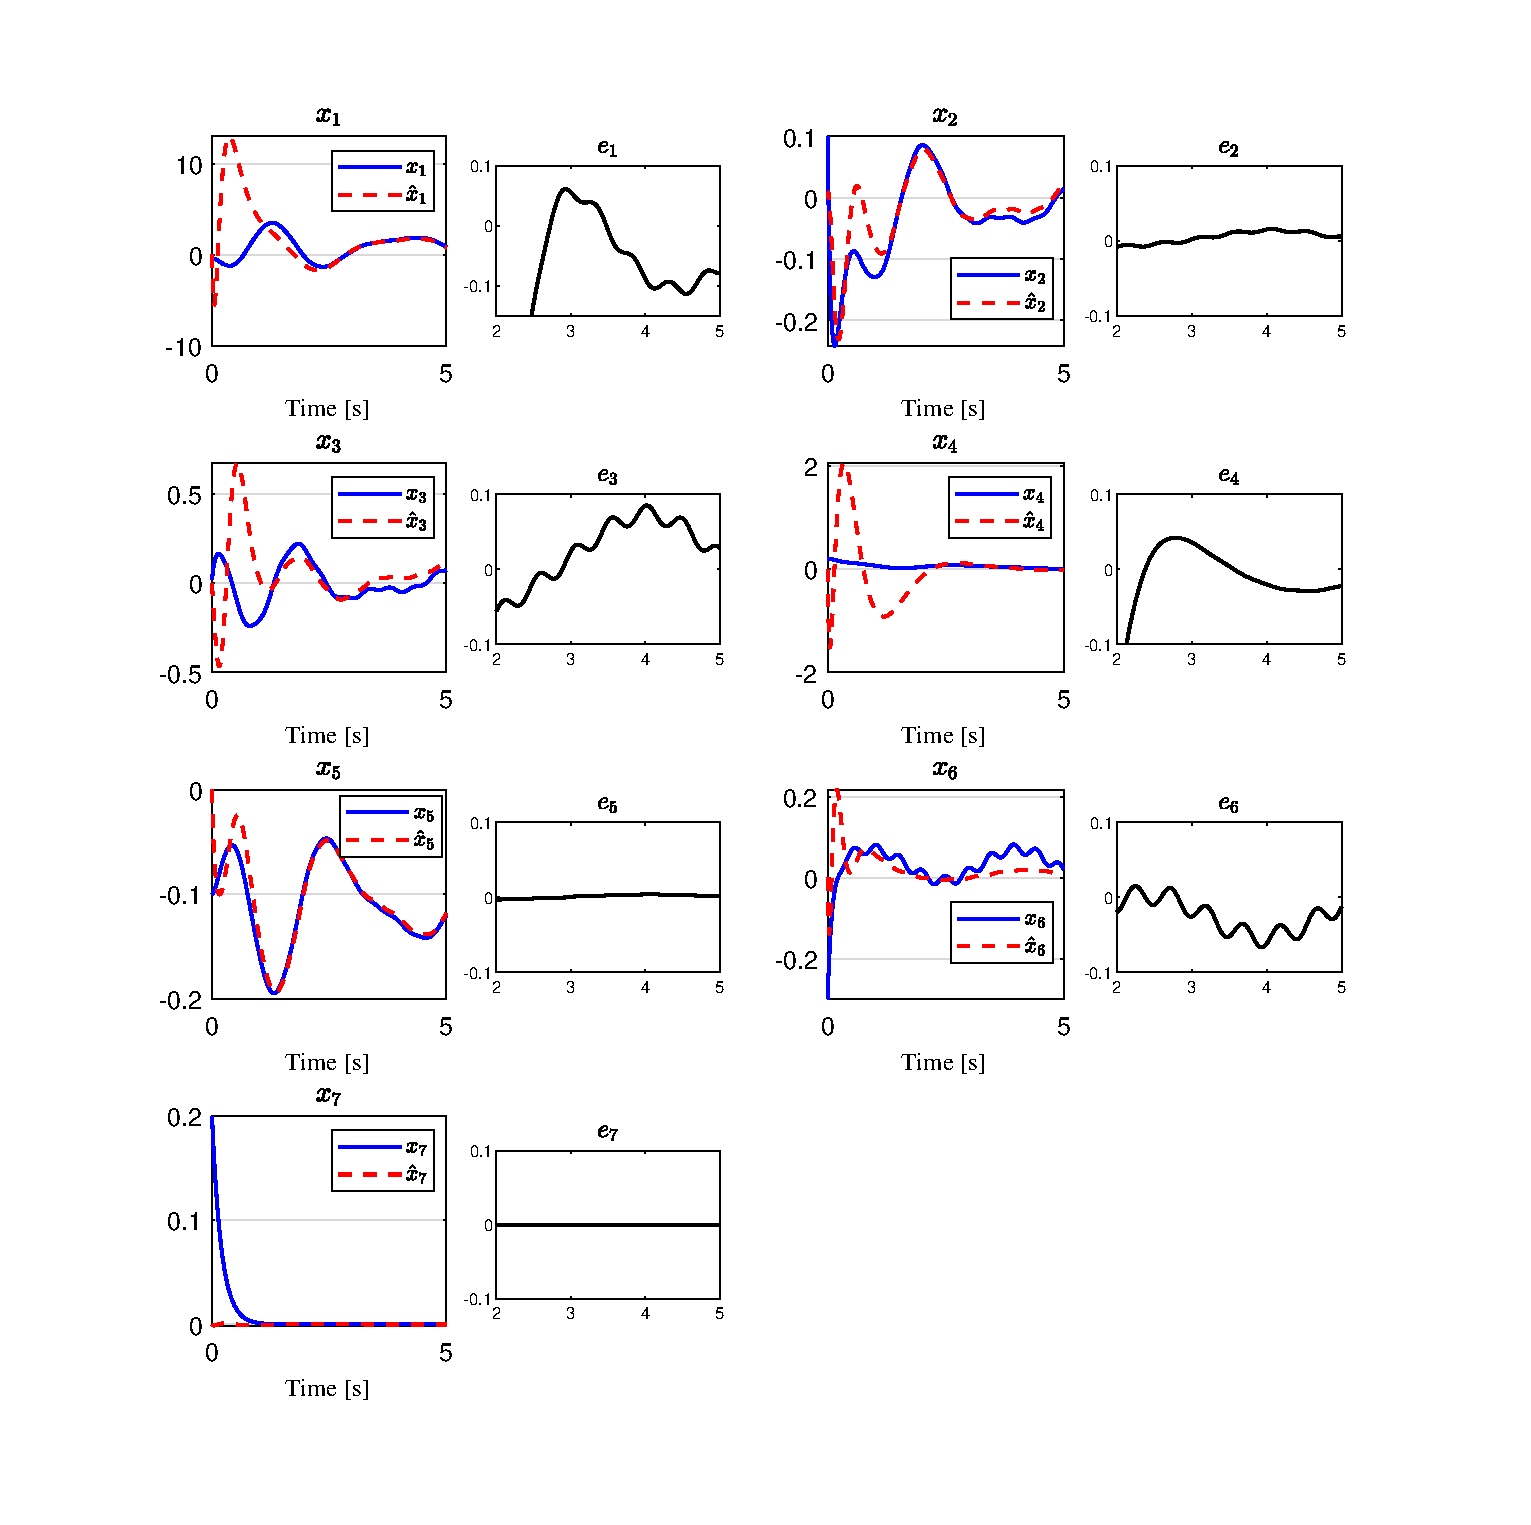
\includegraphics[width=17cm]{sys_7s_linear_states.eps}}
% 	\caption[MIMO Linear UIO]{Linear UIO. Plant state $x$, state estimation $\hat{x}$ and estimation errors $e=\hat{x}-x$.}
% 	\label{fig: CH4 Error states and norm, e_0 linear}
% \end{figure}

% \begin{figure}[htbp]
% 	\centering{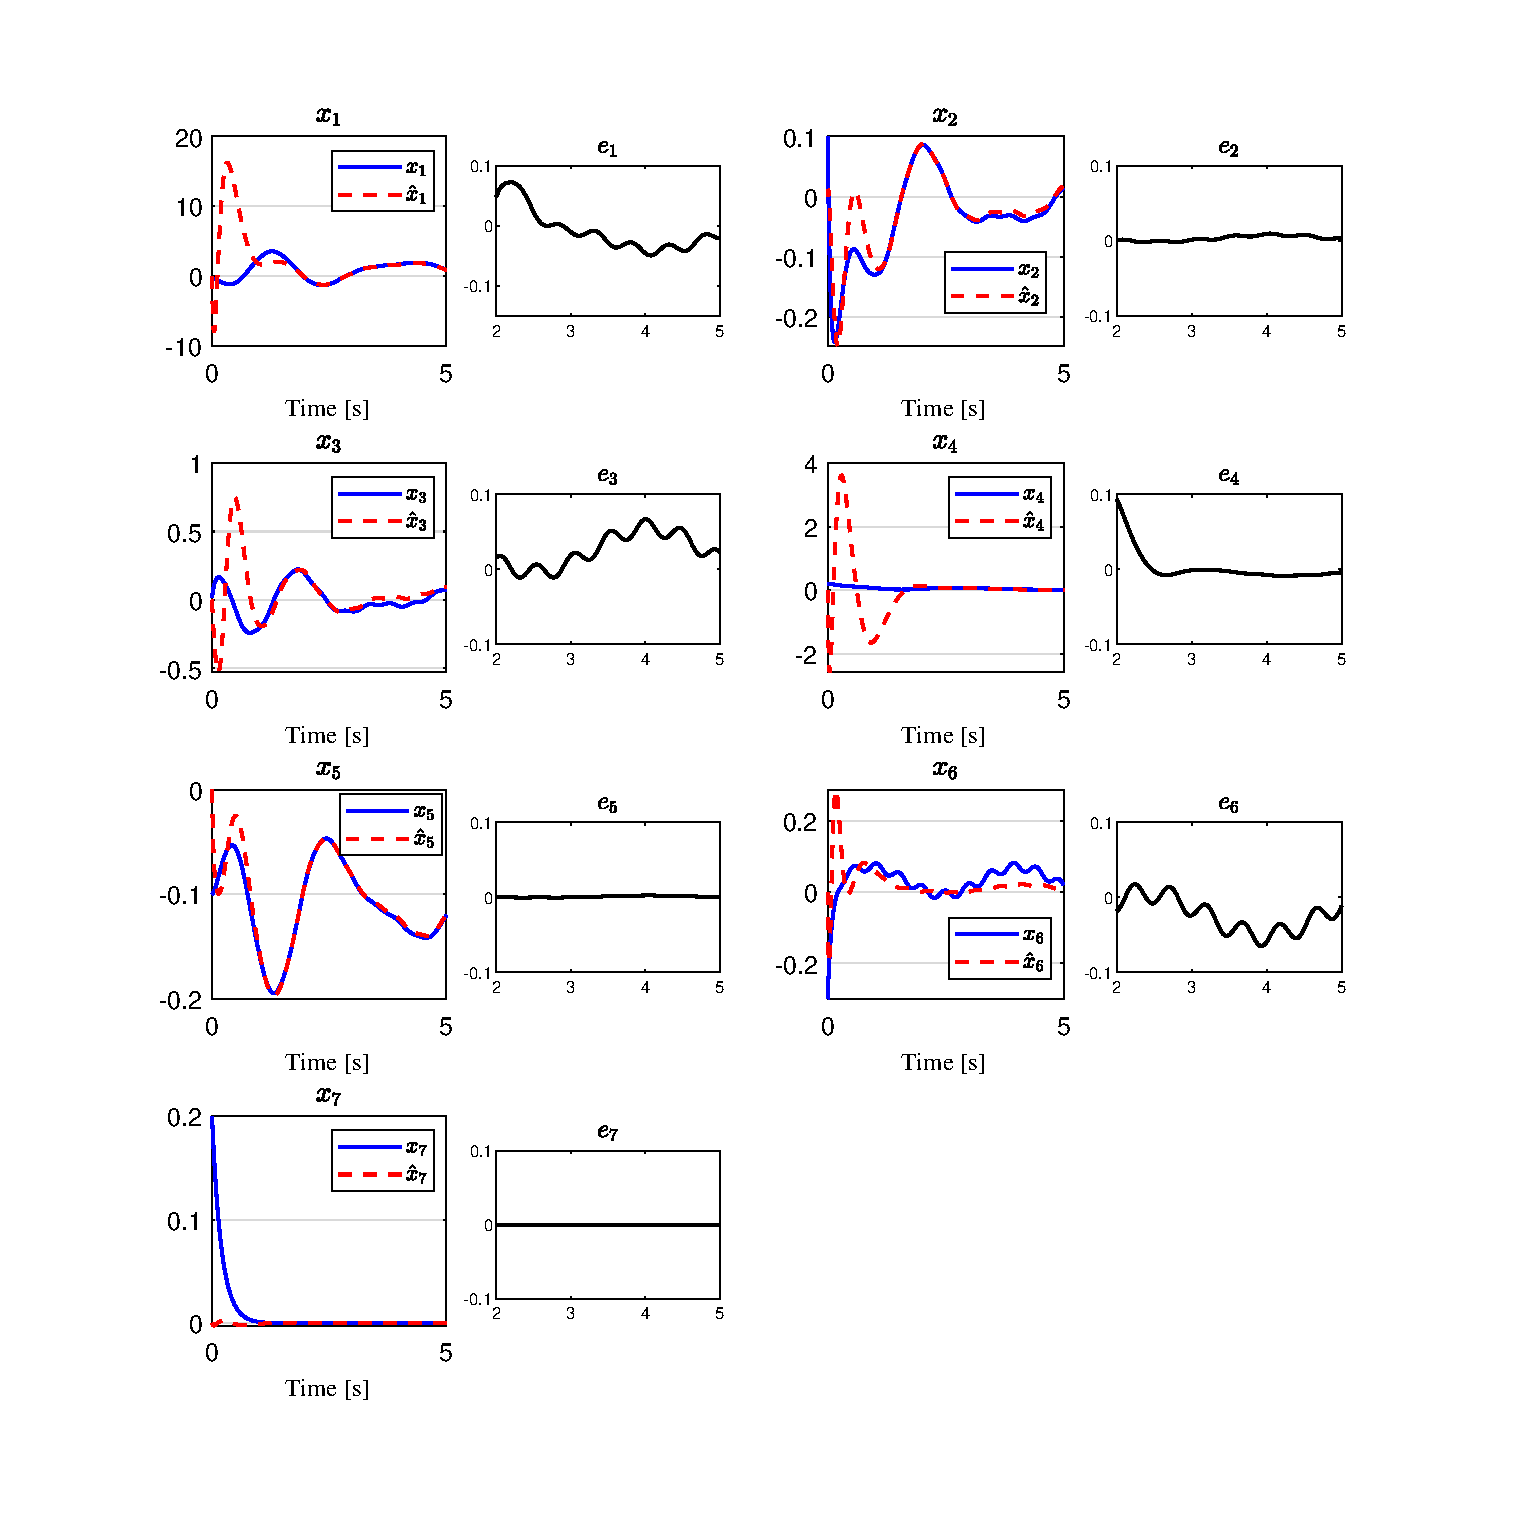
\includegraphics[width=17cm]{sys_7s_cont_states.eps}}
% 	\caption[MIMO Continuous UIO]{Continuous UIO. Plant state $x$, state estimation $\hat{x}$ and estimation errors $e=\hat{x}-x$.}
% 	\label{fig: CH4 Error states and norm, e_0 cont}
% \end{figure}

% \begin{figure}[htbp]
% 	\centering{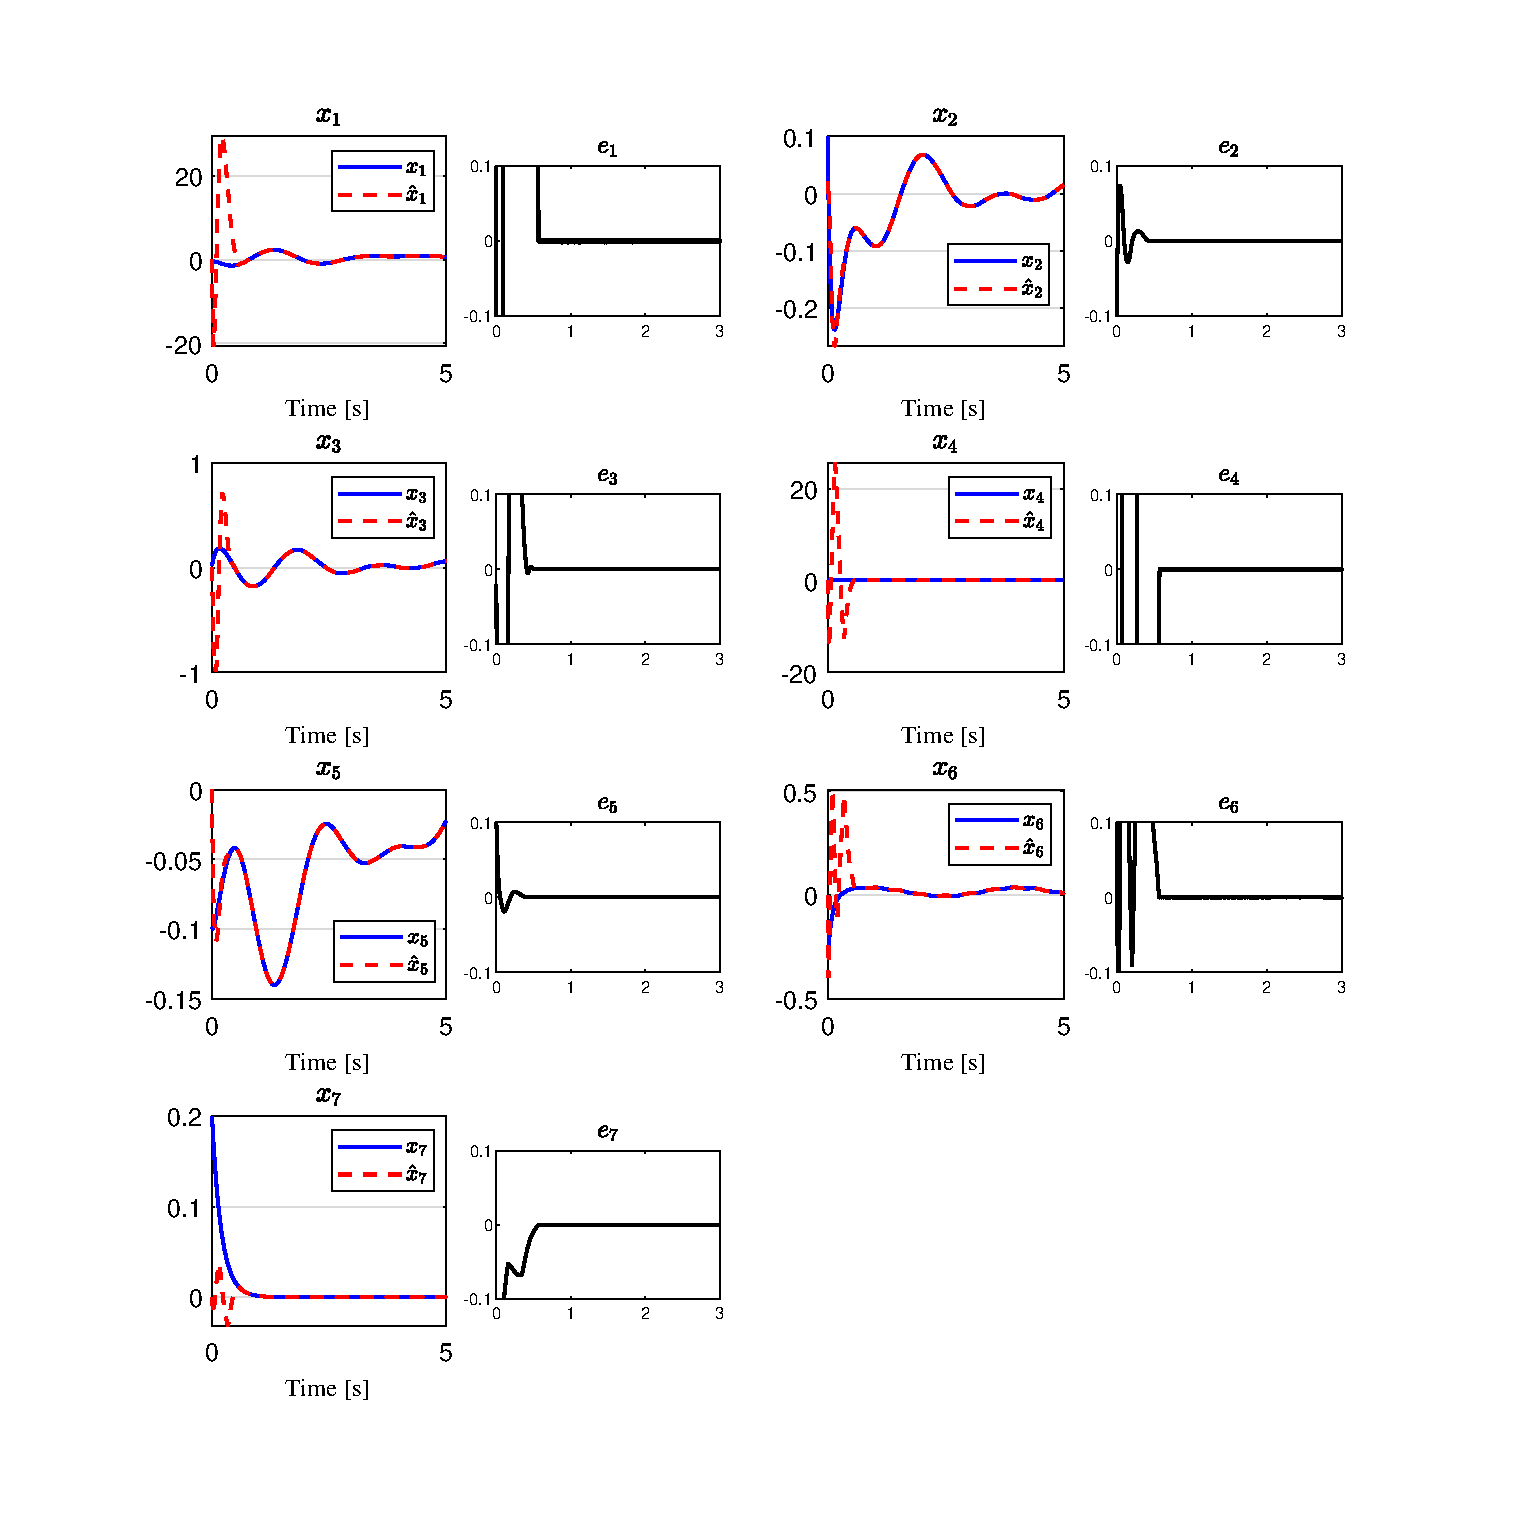
\includegraphics[width=17cm]{sys_7s_disc_states.eps}}
% 	\caption[MIMO HOSM-UIO]{HOSM-UIO. Plant state $x$, state estimation $\hat{x}$ and estimation errors $e=\hat{x}-x$.}
% 	\label{fig: CH4 Error states and norm, e_0 disc}
% \end{figure}

% On the other hand, in the third case with $d_0=-1$ (discontinuous observer), the induced HOSM  allows the observer to compensate exactly the unknown input effect. It is shown in Figure \ref{fig: CH4 Error states and norm, e_0 disc}, that after 0.5s exact convergence of the error norm to zero even in presence of unknown input is achieved, therefore, the states are estimated exactly in finite time.

% In all cases, with appropriately gains selection the error converges to a neighborhood of zero in about one second but it is not clear what happens when the initial estimate is not close to the true state. For the third case, i.e. with $d_0=-1$, $d_{\infty}=\tfrac{1}{9}$ and setting now $L=5,\alpha=10$ we run a set of simulations, Figure \ref{fig: CH4 Error norm with orders} shows the norm of the error vector over a wide range orders of initial estimation error. Here, the error converge to zero in less than 4s for all cases.

% In other words, we achieve more than finite-time, fixed-time stability of the estimation error, i.e. regardless of the initial magnitude of the error, the observer converges before certain time value $\bar{T}$, in this case we can see that the value of this upper cote of estimation time is $\bar{T}=4s$, but this can be reduced arbitrary by increasing appropriately the value of parameter $L$ as we said in the parameters tuning section.

% \begin{figure}[htbp]
% 	\centering{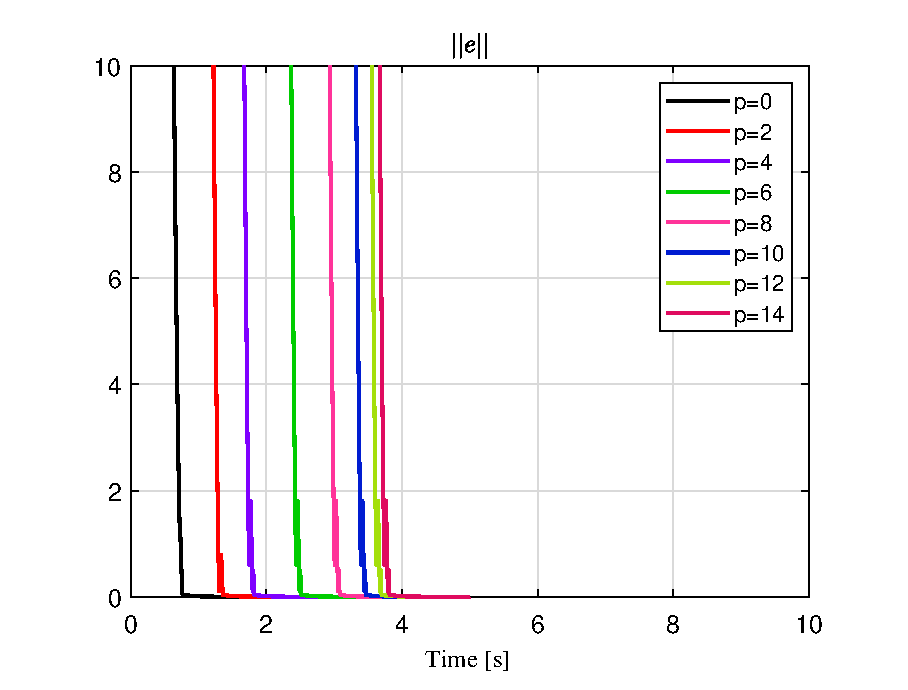
\includegraphics[width=9cm]{sys_7s_disc_FxT_error_orders.eps}}
% 	\caption[MIMO HOSM-UIO Fixed-Time estimation]{HOSM-UIO. Estimation error with different orders at initial error $e_0$ showing fixed-time estimation. With \\ $\hat{x}_{0,j}=1\times 10^{p},j=1,...,7$.}
% 	\label{fig: CH4 Error norm with orders}
% \end{figure}






\chapter{Conclusions}



%%%%%%%%%%%%%%%%%%%%%%%%%%%%%%%%%%%%%%%%%%%%%%%%%%%%%%%%%%%%%
%%
%%			Ejemplo empieza
%%
%%%%%%%%%%%%%%%%%%%%%%%%%%%%%%%%%%%%%%%%%%%%%%%%%%%%%%%%%%%%%%%


% In this work we have proposed a family of observers for state estimation of strongly observable SISO and MIMO Linear Time Invariant systems, the proposed scheme has bl-homogeneous properties, which allow us to assign behavior near and far from the origin independently, this feature allows us the possibility of accelerating when possible the convergence velocity of the observer achieving finite time or more fixed-time convergence. Additionally, the induced HOSM at the origin allow us to deal with bounded unknown inputs having theoretically exact convergence.

% The tuning parameters of the observer are composed by a set of gains, which have an intuitive roll each one, the internal gains $\kappa_{\psi,j},\theta_{psi,j}$ with $\psi=\{(b,\iota),(d,i)\}$ give a relative weight of the low degree terms and the high degree ones in the nonlinear injection terms. The external gains $k_{\psi,j}$ are responsible for ensuring stability of the observer considering absence of interconnections and perturbations, and finally the gains $L,\alpha$ are in charge of dealing with the interconnection and unknown inputs terms respectively by setting them sufficiently large. Thus, the tuning procedure of the observer is simple and structured.

% The boundedness of the state variables is not required for global finite-time or fixed-time stability of the estimation error dynamics which allows for its application to unstable plants.

% In the SISO case the state estimation for LTI systems with unknown inputs problem can be solved by directly applying a HOSM differentiator (like Levant's RED) if we put the system in observer form. Nevertheless, this idea can not be applied if the system is in observability form, since to have global convergence we should have bounded state variables, and this reduces its applicability. In the MIMO case this problem is the same, extended to a set of subsystems. Base on this problem, the construction of bl-homogeneous observers allow us to deal with unbounded functions far of the origin, i.e. with $d_{\infty}\geq 0$ we can deal with Lipschitz and then linear functions of the states in last channel of each subsystem and in the case of selecting $d_0=-1$ we have proof that the observer can deal with the effect of unknown inputs due to the HOSM, obviously, in the absence of unknown inputs a linear $d_0=d_{\infty}=0$ or continuous $-1<d_0< 0 < d_{\infty}$ observer is sufficient to achieve asymptotic or exact and finite time convergence, respectively.

% This work results in a more general observation scheme, with respect to the already existing in literature offering global convergence. In contrast to the cascade scheme \cite{Fridman2006} composed by a Luenberger observer and a HOSM differentiator the structure is much simpler because the order is not unnecessarily increased, therefore the number of parameters is significantly less. Moreover, the Luenberger observer introduce a delay in 
% the estimation, that is avoided in the present scheme.

% On the other hand, for the MIMO case, the observer presented in \cite{Niederwieser2021} is based on a MIMO observer normal form which allows to apply directly an homogeneous differentiator ( Levant's RED is applied), this is because in this observer normal form the resulting subsystems ares interconnected in a convenient form, i.e. the convergence is achieved in a sequential way, when the first subsystem has converged the second one can do, and then sequentially. This observer can not deal with another kind of interconnection terms, for example, those given in observability form. The observer proposed here can deal with both interconnections and in fact, even more general.

% The effectiveness of the observer has been illustrated in the presented examples, both of them have unstable dynamics and bounded unknown inputs. The results showed that, although the unbounded state variables it has global convergence. Also, it was shown that linear and continuous observers cannot completely compensate the effect of unknown inputs, keeping the error in a neighborhood of zero only. But the High Order Sliding Mode produced by having $d_0=-1$ homogeneity degree in the $0$-approximation terms allows the observers to compensate these effects. 

% Although the respective analysis is not addressed in this work, in presence of measurement noise, some extra simulations confirm the robustness of the observation scheme having ISS, that is, the observation error is final and ultimately bounded.

% \section{Future works}
% The present work opens the possibility to several extensions.
% \begin{itemize}
% 	\item Design of bl-homogeneous observers for strongly observable SISO and MIMO Linear Time Variant (LTV) systems, i.e. linear systems whose parameters vary with time. In the SISO case the problem can be stated as the observer design for a system given by
% 	\begin{equation}
% 		\begin{split}
% 			\Sigma: \left\{
% 			\begin{array}{rl}
% 				\dot{x}_{1} &= x_{2}, \quad y=x_{1}, \\
% 				\dot{x}_{j} &= x_{j+1} \\
% 				& \vdots \quad j=2,...,n-1\\
% 				\dot{x}_{n} &= a_{1}(t)x_{1} + a_{2}(t)x_{2} +...+ a_{n}(t)x_{n} + \omega
% 			\end{array}
% 			\right. \\
% 		\end{split}
% 	\end{equation}

% 	\item Design of bl-homogeneous UIO for strongly detectable SISO and MIMO Linear Time Invariant systems, that is, systems with inaccessible but stable internal dynamics. This is an immediate extension that does not require a lot of extra work. For example, in SISO case, the problem boils down to designing observers for systems given by
% 	\begin{equation}
% 		\begin{split}
% 			\Sigma: \left\{
% 			\begin{array}{rl}
% 				\dot{x}_a &= A_{aa}x_a + H_{ad}y\\
% 				\dot{x}_{d,1} &= x_{d,2}, \quad y=x_{1}, \\
% 				\dot{x}_{d,j} &= x_{d,j+1} \\
% 				& \vdots \quad j=2,...,n_{d}-1\\
% 				\dot{x}_{d,n_{b}} &= a_{d,1}x_{d,1} + a_{d,2}x_{d,2} +...+ a_{d,n_d}x_{d,n_d} + \omega
% 			\end{array}
% 			\right. \\
% 		\end{split}
% 	\end{equation}
	
% 	\item The design of bl-homogeneous UIO for nonlinear systems with unknown inputs. Although this issue is currently being addressed by colleagues in the same working group, the MIMO non-linear case is still an undeveloped problem. The problem can be seen as the design of observers for a system given by
% 	\begin{equation}
% 		\begin{split}
% 			\dot{x} &= f(t,x,u)+g(x)\omega(t), \quad x(0)=x_0 \\
% 			y &= h(x)
% 		\end{split}
% 	\end{equation}
	
% 	\item Design of UIO for networks of non-linear systems in general. The methodology presented in this work in the MIMO case under the SCB transformation is a first approach in the development of this topic, since it can be seen as the design of observers for linear subsystems with also linear interconnections in the states. That is, for future works the task can be extended to the development of observers for more general systems with non-linear interconnection functions between them. The problem can be stated a the design for a general system $\Sigma$ given by $N$ non-linear systems with interconnection terms $\Psi_i(\cdot)$ and unknown inputs $\omega(t)$.
% 	\begin{equation}
% 		\begin{split}
% 			\Sigma_i: \left\{
% 			\begin{array}{rl}
% 				\dot{x}_i & = F_i(x_i,u_i) + \Psi_i(x_1,...,x_ N) + G(x_i)\omega_i(t), \quad x_i(0)=x_{i,0} \\
% 				y_i & = H_i(x_i), \quad i=1,...,N
% 			\end{array}
% 			\right. \\
% 		\end{split}
% 	\end{equation}
% 	$\Psi_i(\cdot)$ is an interconnection function that contains all the states $x_i \in \mathbb{R}^{n_i},i=1,...,N$.
% \end{itemize}



%====================================================================
%                                                                 Bibliografia
%====================================================================
\bibliographystyle{apalike} 
\bibliography{Citas}

\end{document}